\documentclass[a4paper,norsk,11pt,twoside]{report}
\usepackage[latin1]{inputenc}
\usepackage[T1]{fontenc}
\usepackage[english]{babel}
\usepackage{epsfig}
\usepackage{graphicx}
\usepackage{amsmath}
\usepackage{pstricks}
\usepackage{subfigure}
\usepackage{hyperref}
\usepackage{epstopdf}
\usepackage{simplewick}
\usepackage{color}
\usepackage{listings}
\lstset{ %
language=C++,                % choose the language of the code
basicstyle=\footnotesize,       % the size of the fonts that are used for the code
numbers=left,                   % where to put the line-numbers
numberstyle=\footnotesize,      % the size of the fonts that are used for the line-numbers
stepnumber=1,                   % the step between two line-numbers. If it is 1 each line will be numbered
numbersep=5pt,                  % how far the line-numbers are from the code
backgroundcolor=\color{white},  % choose the background color. You must add \usepackage{color}
showspaces=false,               % show spaces adding particular underscores
showstringspaces=false,         % underline spaces within strings
showtabs=false,                 % show tabs within strings adding particular underscores
frame=single,           % adds a frame around the code
tabsize=2,          % sets default tabsize to 2 spaces
captionpos=b,           % sets the caption-position to bottom
breaklines=true,        % sets automatic line breaking
breakatwhitespace=false,    % sets if automatic breaks should only happen at whitespace
escapeinside={\%*}{*)}          % if you want to add a comment within your code
}
\usepackage[]{algorithm2e}
\usepackage{tikz}
\usetikzlibrary{arrows,matrix,positioning}

\date{}
\title{}
\author{}

% romersk numerering med arabisk på starten
% arabiske tall når jeg starter selve kapitelene
% \newpage foran hver kapitell ca

\begin{document}


%Forside
\thispagestyle{empty}
\begin{center}        % Sentrerer teksten
  %Tittel
  \vspace{5mm}          % Vertikalt mellomrom
  \LARGE
  \textbf{Coupled Cluster Studies in Computational Chemistry} \\
  \Large
  \vspace{5mm}
  \textbf{by} \\
  \vspace{5mm}
  %Forfatter
  \large
  \textbf{Ole Tobias B. Norli} \\
  %Avdeling for mekanikk
  \vspace{30mm}
  \Large
  {\bf{\textsl{THESIS}}} \\
  \textsl{for the degree of} \\
  \vspace{2mm}
  %%%%%%%OLD%%%%%%{\bf{\textsl{CANDIDATUS SCIENTIARUM}}} \\
  {\bf{\textsl{MASTER OF SCIENCE}}} \\
  \vspace{5mm}
  {\large \textsl {(Master in Computational Physics)}}\\
  \vspace{10mm}
  \centerline{
\includegraphics[width=4cm,height=4cm]{UiO_Segl_cmyk.eps}}
  \vspace{5mm}
  % \textsl{Mechanics Division, Department of Mathematics} \\
  \textsl{Faculty of Mathematics and Natural Sciences} \\
  \textsl{University of Oslo} \\
  %Maaned, aar
  \vspace{10mm}
  \large
  \textsl{August 2014} \\
  \vspace{5mm}
  \normalsize
  % \textsl{Avdeling for mekanikk, Matematisk institutt} \\
  \textsl{Det matematisk- naturvitenskapelige fakultet} \\
  \textsl{Universitetet i Oslo} \\
\end{center}


\begin{abstract}
In this thesis we explore the Coupled Cluster method in Quantum
Chemistry. We have implemented an effective Coupled Cluster Singles
and Doubles code. We also explore deviations from the true ground
state. For this purpose we have implemented a Coupled Cluster Singles,
Doubles and Triples code. Our results are in agreement with theory
that Coupled Cluster converge to a fixed number when including more
excitations and improving the basis set. \\

Our code performance is approaching the level of the best performing
software available. Further continuations of already implemented
optimizations are proposed to help development of more effective
Coupled Cluster code.
\end{abstract}

\renewcommand{\abstractname}{Acknowledgements}
\begin{abstract}
I would like to acknowledge my supervisor Morten H. Jensen. You are the best supervisor I could ask for, thank you. Also thank you to Diako Darian. 
\end{abstract}


\tableofcontents{}

\maketitle
\newpage




\chapter{Introduction}

Quantum Chemistry is a field of research where quantum mechanics is
used to describe the behaviour of atoms and molecules. This can be
used to model for example chemical reactions. A good understanding of
chemical reactions is vitally important in several fields, from
materials science to life science and medicine, with a huge potential
for industrial applications. To develop accurate many-body methods
which allow us to reproduce and predict properties of atoms and
molecules is thus extremely important for scientific progress in a
wide range of scientific fields, from basic research to industrial
applications.\\

In 2013 Martin Karplus and Michael Levitt were awarded the Nobel Prize
in chemistry for their development of multiscale models for complex
chemical systems. Their work focused on Molecular Dynamics (MD)
simulations of large chemical reactions. An important breakthrough in
their work was combing higher and lower accuracy methods to provide an
accurate and computationally efficient model. The active parts of the
molecule were described with high accuracy, while the inactive parts
were described with less accurate methods. \\

In this thesis we will focus on a high accuracy method in quantum
chemistry. We will study the Coupled Cluster method. The Coupled Cluster method is one of the highly successful so-called first-principle methods (or {\em ab initio} methods) and  
was introduced in the late 1950s by Coester and K\"ummel within the context of nuclear physics. 
It was introduced in quantum chemistry in the 1960s by Cizek and Paldus. 
It is considered
to be a highly accurate many-body method. In the 1980s through 1990s several
computational chemists predicted Coupled Cluster would be the method
of choice for most calculations in quantum chemistry today. However
the method applied in the absolute majority of publications is 
Density Functional Theory (DFT).  \\

The main reason DFT is so popular is the computational
affordability. DFT can model much larger systems than Coupled Cluster theory,
and in much less time. Therefore we will focus much of our attention
on implementing an optimized Coupled Cluster code. \\

In this thesis we will develop computational chemistry methods based
on quantum mechanics. These are called ab initio quantum chemistry
methods. We will implement Hartree Fock (HF) theory, Coupled Cluster Singles
and Doubles (CCSD) and Coupled Cluster Singles, Doubles and Triples
(CCSDT) from scratch. We will design parallel algorithms for HF and
CCSD. Our algorithms will focus on effective memory distribution and
high performance. Calculations will be performed on the Abel supercomputing
cluster of the University of Oslo. In particular the CCSD implementation will be greatly
optimized. We will also present an extremely optimized algorithm for
transformation of the four index integrals involved in post-HF
methods. \\

We have benchmarked our performance and results against existing
software. Since our implementation is made from scratch we will also
propose further optimizations in great detail. The proposed
optimizations combine positive features from our implementation and
existing software developed by others. The main purpose will be
working towards a more computationally affordable CCSD
implementation. One that can also run calculations on larger
molecules. \\

We will not present an optimized CCSDT implementation. CCSDT is
implemented to better study the limitations on accuracy in
CCSD. The Coupled Cluster method in theory only contains two errors. These are a
limited basis set and a truncation of excitations included. With CCSDT
implemented we will be able to study both these errors. \\

The thesis is structured for a good presentation of theory, code
development and results. Chapter 2 describes the basics of the system
we will study. The theoretical derivation of the Hartree Fock method
using Gaussian Type Orbitals is given in chapters 3 and 4. \\

Chapter 5 contains a derivation of the CCSD method. In Chapter 6 we provide
the factorized and implementation ready CCSD equations. \\

Chapter 7 contains information about the general programming
principles we will apply in our implementation. This includes
information on parallel programming and external libraries in
use. Chapter 8 discusses our actual serial and parallel
implementation of HF theory and CCSD.\\

Chapter 9 is an implementation guide to the CCSDT method. We will not
derive the equations for this method. Multiple references are included
and the equations are presented in an implementation ready form. Our
actual implementation of CCSDT is plain and simple, as presented
in this chapter. \\

In chapter 10 we present benchmark calculations to validate our
implementation. Chapter 11 presents new results and chapter 12 states our
conclusions. In chapter 13 we propose future prospects. 



\chapter{Definition of Hamiltonian}

In this chapter we present the Hamiltonian, with some basic definitions, for the systems we want to
study in this thesis, namely various atoms and molecules (with an emphasis on molecules) 
using first principle theories. We are mainly
interested in the ground state of atoms and molecules, and we aim at 
solving the time-independent Schr\"odringer equation
\begin{equation}
\textbf{H} |\Psi \rangle = E |\Psi \rangle,
\end{equation}
where $\textbf{H}$ is the Hamiltonian of the system, $\Psi$ the given eigenstate function and $E$ the corresponding
eigenenergy or simply energy  of the system. 

\section{Hamiltonian}
The full Hamiltonian for such atoms and molecules  is well defined, it reads
\begin{align}
\textbf{H} = &
- \sum_A^{nuc} \frac{1}{2m_A} \nabla_A^2
- \sum_i^E \frac{1}{2} \nabla_i^2
- \sum_A^{nuc} \sum_i^E \frac{Z_A}{|r_i - R_A|}
\nonumber \\ &
+ \sum_{i>j}^E \frac{1}{|r_i - r_j|}
+ \sum_{A>B}^{nuc} \frac{1}{|R_A - R_B|}.
\end{align}
The various terms represent the kinetic and potential energy terms for the electrons and the nucleus (in case of atoms) or nuclei in case of molecules. Here $R_A$ is the position of a given nucleus, $r_i$ is the position of electron $i$, $m_A$ is the mass ratio of a given given nucleus with the electron mass and $Z_A$ is the charge of that specific nucleus.


\section{The Born-Oppenheimer approximation}
Throughout this thesis we will employ a Hamiltonian where the
Born-Oppenheimer approximation is used.  In this approximation we
neglect the nuclear kinetic energy, since the time it takes for a
nucleus to move is large compared to the time it takes for the
electrons to obtain their ground state configuration. This means we
can solve the equations first with the nucleus or the nuclei at fixed
positions. When the nucleus (or nuclei in case of molecules) is (are)
at a fixed position the kinetic energy term becomes zero. We neglect
also contributions from nuclear forces since their energy scales are
in the gigaelectronvolt domain. We will refer to such a Hamiltonian as
the electronic Hamiltonian, $\textbf{H}_e$, and it reads
\begin{equation}
\textbf{H}_e = - \sum_i^E \frac{1}{2} \nabla_i^2
- \sum_A^{nuc} \sum_i^E \frac{Z_A}{|r_i - R_A|}
+ \sum_{i>j}^E \frac{1}{|r_i - r_j|}
+ \sum_{A>B}^{nuc} \frac{1}{|R_A - R_B|}.
\end{equation}
The term $\frac{1}{|R_A - R_B|}$ has no electrons in it, but it is
often included in the electronic Hamiltonian. With nuclei at fixed
positions this term reduces to a constant value. Using the
electronic Hamiltonian we can then find the potential energy of the
nuclei. \\

In this thesis we will thus only be working with the electronic
Hamiltonian, and in future chapters we will just call it $\textbf{H}$.

\section{Comments on the Wavefunction}
In this thesis we will represent the many-particle state function (or just wavefunction, $\Psi$) by single-particle basis function that solve the Hartree-Fock equations. These equations will be derived in chapter \ref{hf_chapter_reference}. The Hartree-Fock method represents an
approximation to the solution of the full Schr\"odinger equation. \\

In
practical terms, it is an algorithm which allows us to rewrite the abovementioned many-particle Schr\"odinger 
equation in terms of coupled single-particle equations. It represents perhaps the simplest approach to the 
full many-body problem and provides a so-called self-consistently solved  basis of orthogonal single-particle wavefucntions. We will call these single-particle states for spin orbitals hereafter. 
These basis functions are in turn used as input to so-called post Hartree-Fock methods like many-body perturbation
theory or coupled-cluster theory discussed in more detail in this thesis. \\

 In the Hartree-Fock approximation we assume that the many-body wavefunction can be
written as a function of single electron wavefunctions. Each electron
will occupy its own spin orbital. Since we are aiming at the ground state, the
occupied spin orbitals are the ones with the lowest energy from the solution of the Hartree-Fock equations.\\

\begin{figure}[ht!]
\centering
\includegraphics[width=90mm]{tat.jpeg}
\caption{Illustration of electrons occupying orbitals to construct a wavefunction.}
\label{fig:basic_kapitell1_fig}
\end{figure}

Figure \ref{fig:basic_kapitell1_fig} is an illustration of
this. The state $|\Psi_0 \rangle$ has six electrons. Two electrons occupy the
lowest orbital in energy, one with spin up and one with spin down. Two electrons
occupy the second lowest orbital in energy, and the last two electrons occupy the third
lowest energy level. This forms then an ansatz for  the ground state. The next wavefunction has a
configuration where one electron can be  excited to a higher energetic
orbital. This is labeled as $| \Psi_i^a \rangle$. \\

We here use a standard quantum chemistry notation, where
occupied spin orbitals are labeled by the letters $i,j,k,\dots$ and unoccupied orbitals are labeled as 
$a,b,c,\dots$. 
The occupied spin orbitals serve to define the ansatz for the ground state wave function, in our case this will be a 
so-called Slater determinant since our particles (the electrons) are fermions and need to obey the requirement that the 
total wavefunction is antisymmetric in space. 
A generic spin orbital is labeled by the letters $p,q,r,\dots$. Any electron can be
excited to any of the higher orbitals. The state $|\Psi_{ij}^{ab} \rangle$
represents two electrons excited to higher energetic orbitals. \\

To find the true electronic wavefunction we would need a perfect
description of the orbitals, and a linear combination of all the
different possible excitations. There is an unlimited number of
possible excitations, but some are more likely than others. In Coupled
Cluster theory, to be discussed later, we will include some of these excited states. 




\chapter{Hartree Fock \label{hf_chapter_reference}}
In this chapter we will discuss the Hartree-Fock (HF) method. We will
derive the HF equations. For the most part we will limit ourselves to
deal with a spin restricted HF (RHF) method, with closed shells and a
single Slater determinant, Ref.~\cite{slater_determinant_new_citation}, approximation to the wavefunction. However a
spin unrestricted version has also been implemented and will be
discussed briefly. \\

Much of the material discussed here is based on a series of summer lectures
series from the Sherill Group, see for example Ref.~\cite{ref111111}, but see also 
Ref.~\cite{ref222222} for further details. Additional references include the recent Master of Science theses from the 
Computational Physics group at the University of Oslo, see the theses of
S.~A.~Dragly \cite{sadragly}, H.~M.~Eiding \cite{hmeiding} and M.~H.~Mobarhan \cite{mhmobarhan}. 
This chapter is also closely
related to the following chapter on an optimal basis for atoms and molecules, the so-called  Gaussian Type Orbitals (GTO).

\section{Introduction}
Since our main focus is on molecules, in our exposition of  
the HF method we will describe how to approximate the Schr\"odringer equation for an arbitrary molecule. 
Our equation in atomic units reads	

\begin{equation}
\textbf{H} | \Psi \rangle = E | \Psi |\rangle,
\label{hartreefock_1}
\end{equation}
where our electronic Hamiltonian, $\textbf{H}$, is defined

\begin{equation}
\textbf{H} = 
- \sum_i \frac{1}{2} \nabla_i^2 
- \sum_{iA} \frac{Z_A}{r_{iA}}
+ \sum_{i>j} \frac{1}{r_{ij}} 
+ \sum_{AB} \frac{Z_A Z_B}{R_{AB}} .
\end{equation}
Here $Z_A$ is the atomic number of nucleus A (with charge in atomic units) 
and $r_{iA}$ is the distance from nucleus A to electron i. 
To simplify notation we will introduce two new operators, $\textbf{h}(i)$ and $\textbf{v}(i,j)$. These are defined by

\begin{equation}
\textbf{h}(i) = - \frac{1}{2} \nabla_i^2 - \sum_A \frac{Z_A}{r_{iA}}, \label{single_particle_hf}
\end{equation}
which defines the one-body (or single-particle) electron Hamiltonian and

\begin{equation}
\textbf{v}(i,j) = \frac{1}{r_{ij}},
\end{equation}
which is called the two electron part of our Hamiltonian. The quantity
$r_{ij}$ is defined as the distance between electron i and electron
j. $r_{ij} = |r_i - r_j|$. This quantity has the following symmetry
$r_{ij} = r_{ji}$, and has the constraint that $i \not= j$. We also
introduce a shorthand notation for the nucleus-nucleus repulsion, namely,

\begin{equation}
V_{NN} = \sum_{AB} \frac{Z_A Z_B}{r_{AB}}.
\end{equation}
This leaves Eq.~\eqref{hartreefock_1} as

\begin{equation}
\left( 
\sum_i \textbf{h}(i) + \frac{1}{2} \sum_{ij} \textbf{v}(i,j) + V_{NN}
\right) | \Psi(R) \rangle
= E | \Psi(R) \rangle.
\end{equation}
Here $R$ is a vector of Cartesian coordinates (x, y, z) and spin for
the different electrons. We have also included a factor $\frac{1}{2}$
since we removed the constraint $i > j$ from the sum.

\section{Slater Determinant}
The first assumption made in HF theory is that the wavefunction, $\Psi(R)$,
can be written as a single Slater determinant. A Slater determinant is
defined as

\begin{equation}
\Psi_T(R) = \frac{1}{\sqrt{N!}}
\begin{vmatrix} 

        \psi_1(x_1) & \psi_2(x_1)  & \psi_3(x_1) & \dots  & \psi_N(x_1) \\ 
        \psi_1(x_2) & \psi_2(x_2)  & \psi_3(x_2) & \dots & \psi_N(x_2) \\
        \psi_1(x_3) & \psi_2(x_3)  & \psi_3(x_3) & \dots & \psi_N(x_3) \\
        \dots & \dots & \dots & \dots & \dots \\
        \psi_1(x_N) & \psi_2(x_N)  & \psi_3(x_N) & \dots & \psi_N(x_N) \\

    \end{vmatrix}
    .
\end{equation}
Here $N$ is the number of electron and $x_i$ denotes the $x$, $y$ and
$z$ coordinates for a single electron, i = 1, 2, $\dots$. The subscript $T$ in $\Psi_T$
indicates that this is a trial wavefunction, and not the exact
one. The factor $\frac{1}{\sqrt{N!}}$ is a normalization factor.  \\

An orbital is the wavefunction for a single electron. An atomic orbital is the wavefunction for a single electron in an atom. A molecular orbital is the wavefunction of a single electron in a molecule. \\

A spacial orbital is an orbital that describes the position of an
electron. A spin orbital describes the position and the spin of an
electron. Each spacial orbital has two spin orbitals, since electrons
are fermions with spin up or spin down. The quantity $\psi_i$ represents a
molecular spin orbital, in case of molecules. \\

There are a few properties that make a Slater determinant an
attractive trial wavefunction. First, it is antisymmetric, which means
a change in sign upon interchanging two particles. Second it
incorporates the Pauli Exclusion Principle, whose consequence states
that two identical fermions cannot occupy the same state
simultaneously.  \\

For our purposes we approximate $\Psi$ with a single Slater
determinant. A single Slater determinant is a so called independent
particle approximation. This will be discussed later in more depth. \\

Another shorthand notation for $\Psi_T(R)$ we will use soon is

\begin{equation}
| \Psi_T(R) \rangle = |i j k l \dots \rangle, 
\label{hfnotat}
\end{equation}
where index i, j, k, l, $\dots$ refer to a molecular spin orbital.

\section{The Energy Expression}
We will now find an expression for the energy with this wavefunction. The energy can be found by rewriting Eq. \eqref{hartreefock_1}, namely. 

\begin{align}
E^{HF} & = \langle \Psi_T | \textbf{H} | \Psi_T \rangle \nonumber \\ &
= \langle \Psi_T | \left( \sum_i \textbf{h}(i) + \frac{1}{2} \sum_{ij} \textbf{v}(i,j) + V_{NN} \right) | \Psi_T \rangle \nonumber \\ &
= \langle \Psi_T | \sum_i \textbf{h}(i) | \Psi_T | \rangle
+ \frac{1}{2} \langle \Psi_T | \sum_{ij} \textbf{v}(i,j) | \Psi_T \rangle
+ \langle \Psi_T | V_{NN} | \Psi_T \rangle.
\label{hfref2}
\end{align}
Here we have labeled the energy  as $E^{HF}$ in order to stress that it is the Hartree Fock energy we are aiming at. 
We also split up the equations into three parts. The easiest one comes from the nucleus-nucleus repulsion,

\begin{equation}
\langle \Psi_T | V_{NN} | \Psi_T \rangle = V_{NN} \langle \Psi_T | \Psi_T \rangle
= \sum_{AB} \frac{Z_A Z_B}{r_{AB}}.
\end{equation}
This will be a constant number. For the other two terms we use the
attributes of the Slater determinant to simplify. We also insert the
alternative notation noted in Eq. \eqref{hfnotat} and have

\begin{align}
\langle \Psi_T | \textbf{h}(i) | \Psi_T \rangle
 = \langle i j k l \dots | \textbf{h}(i) | i j k l \dots \rangle .
\end{align}
The operator $\textbf{h}(i)$ acts only on one orbital at the time, namely orbital $i$. The properties of the Slater determinant are such that this simplifies to

\begin{equation}
\langle i j k l \dots | \textbf{h}(i) | i j k l \dots \rangle = \langle i | \textbf{h} | i \rangle .
\end{equation}
The expression for the two-electron operator simplifies to

\begin{equation}
\langle i j k l  \dots | \textbf{v}(i,j) | i j k l \dots \rangle = \langle ij || ij \rangle .
\end{equation}
Notice that only two electrons are involved since we only have a two-body operator at most in our Hamiltonian. 
Here $\langle ij || ij \rangle$ is a shorthand for the double bar integral, defined as

\begin{equation}
\langle ij || ij \rangle = \langle ij | ij \rangle - \langle ij | ji \rangle .
\end{equation}
with $x_i$ being the coordinates and spin of electron $i$. 
Inserting this into Eq.~\eqref{hfref2} gives us

\begin{equation}
E^{HF} = 
\langle i | \textbf{h} | i \rangle 
+ \frac{1}{2} \left( \langle ij | ij \rangle - \langle ij | ji \rangle \right)
+ V_{NN} ,
\end{equation}
with $\langle ij | ij \rangle$ being defined as

\begin{equation}
\langle ij | ij \rangle = \int dx_1 \int dx_2 \psi_i^*(x_1) \psi_j^*(x_2) \frac{1}{r_{12}} \psi_i(x_1) \psi_j(x_2) .
\end{equation}
Note that $\psi_i^*$ and $\psi_i$ takes the same electron as input. Another notation frequently used in quantum chemistry is 

\begin{equation}
\langle ij | ij \rangle = [ii|jj] ,
\end{equation}
or in the case of general spin orbitals $p, q, r, s$ as

\begin{equation}
\langle pq | rs \rangle = [pr|qs] .
\end{equation}
The two-body interaction has several symmetries that we can utilize to improve the performance  of our codes.
One symmetry is given by the relation

\begin{equation}
\langle pq | rs \rangle = \langle qp | sr \rangle . \label{interchangesym} 
\end{equation}
We will use real orbitals. This provides four more symmetries, namely

\begin{equation}
\langle pq | rs \rangle = \langle rq | ps \rangle = \langle ps | rq \rangle = \langle rs | pq \rangle . \label{interchangesym2}
\end{equation}
These four symmetries can also be applied to Eq.~\eqref{interchangesym} which means we have in total eight symmetries..

\section{The Hartree Fock Equations}

To find the lowest possible energy we must find the molecular orbitals
that produce this energy. When finding a minima in such an equation we
employ the method of Lagrangian multipliers. The method is described
in detail in Ref.~\cite{lagrange_duden}. Here we will simply present the
equations for our system, and give some brief arguments  why these terms are
present in the equation

\begin{equation}
\mathcal{L}[\{\psi_i\}] = E^{HF}[\{\psi_i\}] - \sum_{ij} \epsilon_{ij} \left( \langle i | j \rangle - \delta_{ij} \right) . \label{tweakhf}
\end{equation}
Here $\mathcal{L}$ is a functional of the set of $\psi_i$. The aim is to find the minimum of this functional. 
The set of single-particle orbitals $\psi_i$ will be varied in order to find this minimum. The condition $\langle i | j \rangle - \delta_{ij}$ is a constraint we impose to ensure the molecular spin orbitals remain orthonormal, even when we vary them. That is we require

\begin{equation}
\langle i | j \rangle = \delta_{ij} .
\end{equation}
The quantity 
$\epsilon_{ij}$ are the undetermined Lagrange multipliers. The variation in our orbitals can be described as

\begin{equation}
\psi_i \rightarrow \psi_i + \delta \psi_i .
\label{hftweaks}
\end{equation}
We want to find the minimum of the functional $\mathcal{L}$. This means its derivative must be equal to zero, that is

\begin{equation}
\delta \mathcal{L} = 
\delta E^{HF}[\{\psi_i\}] 
- \sum_{ij} \epsilon_{ij} \delta \langle i | j \rangle
= 0 . \label{hflabting}
\end{equation}
We then insert Eq. \eqref{hftweaks} into the two terms in this equation, starting with the final term and obtain

\begin{equation}
\delta \langle i | j \rangle = 
\langle \delta i | j \rangle
+ \langle i | \delta j \rangle
+ \langle \delta i | \delta j \rangle .
\end{equation}
where $\delta i$ represent the variation of a single-particle orbital. With 

\begin{equation}
\delta \langle i | j \rangle \approx 
\langle \delta i | j \rangle
+ \langle i | \delta j \rangle .
\end{equation}
we find the variation in energy $\delta E^{HF}$ as

\begin{align}
\delta E^{HF} = & 
\sum_i \left( \langle \delta i | \textbf{h} | i \rangle
 + \langle i | \textbf{h} | \delta i \rangle \right)
 + \frac{1}{2} \sum_{ij} (
 \langle \delta i j | i j \rangle
 + \langle i \delta j | i j \rangle
 + \langle  i j | \delta i j \rangle \nonumber \\ &
 + \langle  i j | i \delta j \rangle
 - \langle \delta i j | j i \rangle 
 - \langle i \delta j | j i \rangle 
 - \langle i j | \delta  j i \rangle 
 - \langle i j | j \delta i \rangle )
 \nonumber \\ &
 = \sum_i (
 \langle \delta i | \textbf{h} | i \rangle
 + \langle i | \textbf{h} | \delta i \rangle ) \nonumber \\ &
 + \sum_{ij} (
 \langle \delta i j | i j \rangle 
 + \langle  i \delta j | i j \rangle
 - \langle \delta i j | j i \rangle 
 - \langle i \delta j | j i \rangle ) .
\end{align}
Here we used the symmetries defined in Eq. \eqref{interchangesym}. We insert this in Eq. \eqref{hflabting} and get

\begin{align}
0 = & \sum_i (
 \langle \delta i | \textbf{h} | i \rangle
 + \langle i | \textbf{h} | \delta i \rangle )
 - \sum_{ij} \epsilon_{ij} ( \langle \delta i | j \rangle)
+ \langle i | \delta j \rangle )
  \nonumber \\ &
 + \sum_{ij} (
  \langle \delta i j | i j \rangle 
 + \langle  i \delta j | i j \rangle
 - \langle \delta i j | j i \rangle 
 - \langle i \delta j | j i \rangle ) .
 \label{hfeq}
\end{align}
We now examine the term $\sum_{ij} \epsilon_{ij} \langle \psi_i | \delta \psi_j \rangle$. 
We will specifically take its complex conjugate twice, resulting in

\begin{equation}
\sum_{ij} \epsilon_{ij} \langle i | \delta j \rangle
= \left[ \sum_{ij} \epsilon_{ij}^* \left( \langle i | \delta j \rangle \right)^* \right]^* .
\end{equation}
The complex conjugate of the inner product interchanges the bra and
the ket states. We insert this and then interchange the indices $i$ and $j$. We
can make this interchange because we are summing over all possible indices $i$
and $j$, resulting in

\begin{equation}
\left[ \sum_{ij} \epsilon_{ij}^* \left( \langle i | \delta j \rangle \right)^* \right]^* 
= \left[ \sum_{ij} \epsilon_{ij}^*  \langle \delta j | i \rangle \right]^*
=  \left[ \sum_{ij} \epsilon_{ji}^*  \langle \delta i | j \rangle \right]^* .
\end{equation}
We will assume $\epsilon_{ij}$ is part of a hermitian matrix where $\epsilon_{ji}^* = \epsilon_{ij}$. 
We have then 

\begin{equation}
\left[ \sum_{ij} \epsilon_{ji}^*  \langle \delta i | j \rangle \right]^* = \left[ \sum_{ij} \epsilon_{ij} \langle \delta i | j \rangle \right]^* .
\end{equation}
The content inside the parenthesis is the same as the other term
involving $\epsilon_{ij}$ in Eq.~\eqref{hfeq}. We have just shown that
the two terms are the complex conjugate of each other. This will hold
true for all terms in Eq.~\eqref{hfeq}. One term in the equation
is the complex conjugate of another. We will mark this in our equation
as $+ c.c.$, where this represents the complex conjugate of every
single term remaining in Eq.~\eqref{hfeq}. We have then

\begin{equation}
0 =  \sum_i 
 \langle \delta i | \textbf{h} | i \rangle
 - \sum_{ij} \epsilon_{ij} \langle \delta i | j \rangle)
 + \sum_{ij} (
 \langle \delta i j | i j \rangle 
 - \langle \delta i j | j i \rangle  ) + c.c .
\end{equation}
This equation can be rewritten using the definition of the inner product and drawing the sum over i and $\delta \psi_i^*(x_1)$ outside a parenthesis, resulting in 

\begin{align}
0 = & \sum_i \int dx_1 \delta \psi_i^*(x_1) 
\Big[
\textbf{h}(x_1) \psi_i(x_1)
+ \sum_j \psi_i(x_1) 
\int dx_2
\frac{1}{r_{12}} \psi_j^*(x_2) \psi_j(x_2)
\nonumber \\ &
- \sum_j \psi_j(x_1) \int dx_2 \frac{1}{r_{12}} \psi_j^*(x_2) \psi_i(x_2)
- \sum_j \epsilon_{ij} \psi_j(x_1)
\Big]
+ c.c .
\end{align}
We should be able to insert any reasonable set of $\psi_i$ into this equation
and find a minimum of the Lagrangian. This means that the terms inside the
bracket are the ones that should be zero. If the content of the
brackets are zero, then the complex conjugate of this will also be
zero. This may not hold if the content inside the brackets are purely
imaginary. However we will not be dealing with such a situation. \\

We can thus put the content inside the bracket equal to zero, and set
$\psi_j^*(x_2) \psi_j(x_2) = |\psi_j(x_2)|^2$, yielding

\begin{align}
0 = &
\textbf{h}(x_1) \psi_i(x_1)
+ \sum_j \psi_i(x_1) 
\int dx_2
\frac{1}{r_{12}} |\psi_j(x_2)|^2
\nonumber \\ &
- \sum_j \psi_j(x_1) \int dx_2 \frac{1}{r_{12}} \psi_j^*(x_2) \psi_i(x_2)
- \sum_j \epsilon_{ij} \psi_j(x_1) .
\end{align}
We can rewrite the latter as

\begin{align}
\sum_j \epsilon_{ij} \psi_j(x_1) = &
\textbf{h}(x_1) \psi_i(x_1)
+ \sum_j \left[ 
\int dx_2
\frac{1}{r_{12}} |\psi_j(x_2)|^2
\right]
\psi_i(x_1)
\nonumber \\ &
- \sum_j \left[ \int dx_2 \frac{1}{r_{12}} \psi_j^*(x_2) \psi_i(x_2) \right] \psi_j(x_1) .
\label{hfequgogo}
\end{align}
It is common to define two operators, $\textbf{J}$ and $\textbf{K}$, to make this equation more compact. 
These operators are defined as 
\begin{equation}
\textbf{J}_j(x_1) \equiv \int dx_2
\frac{1}{r_{12}} |\psi_j(x_2)|^2 . \label{JJdefinition}
\end{equation}
and
\begin{equation}
\textbf{K}_j(x_1) \psi_i(x_1) \equiv 
\left[ \int dx_2 \frac{1}{r_{12}} \psi_j^*(x_2) \psi_i(x_2) \right] \psi_j(x_1) .
\label{KKdefinition}
\end{equation}
Using these definitions in   Eq.~\eqref{hfequgogo} results in

\begin{equation}
\sum_j \epsilon_{ij} \psi_j(x_1) = 
\left[
\textbf{h}(x_1)  
+ \sum_j \textbf{J}_j(x_1) 
- \sum_j \textbf{K}_j(x_1) 
\right]
\psi_i(x_1)  .
\label{dfjkaahagagyagyaaaaaaffaa}
\end{equation}
The content of the brackets on the right hand side of the equation will be defined as the Fock operator, namely 

\begin{equation}
\textbf{F}(x_1) \equiv \textbf{h}(x_1)  + \sum_j \textbf{J}_j(x_1) - \sum_j \textbf{K}_j(x_1) . 
\end{equation}
Since we require that our single-particle orbitals should be
orthonormal, $\epsilon$ is a diagonal matrix, that is $\epsilon_{ij}
= \delta_{ij} \times \epsilon_i$. This means we can remove the sum
over $j$. The only term to survive on the left hand side of
Eq.~\eqref{dfjkaahagagyagyaaaaaaffaa} is thus given by $i = j$,

\begin{equation}
\textbf{F}(x_1) \psi_i(x_1) = \epsilon_{i} \psi_i(x_1) . \label{insert_here}
\end{equation}
The term $\epsilon_{i}$ becomes the eigenvalues of the Fock
operator. This means we have an eigenvalue problem. The operator
$\textbf{F}$ is defined in terms of $\psi_i$, but to find $\psi_i$ we
need the operator $\textbf{F}$. This is a circular problem, which can
be solved iteratively.

\section{Restricted Hartree Fock}
The Hartree-Fock-Roothan method, Ref.~\cite{rothaan_new_citation}, is one way of
solving the HF equations when the spin is restricted (that is all spin orbitals are occupied, resulting in a total spin and angular momentum equal to zero). What we do is to
choose a basis set of predefined functions that will be our guess for the 
atomic orbitals, $\phi_{\mu}$. These will be discussed in the next
chapter. For the present discussion we simply state that the basis functions we choose are
usually not orthonormal. We want the atomic orbitals to define our
molecular orbitals $\psi_i$, 

\begin{equation}
\psi_i(x_1) = \sum_{\mu}^M C_{i \mu} \phi_{\mu}(x_1) .
\end{equation}
The lefthand side here is a molecular orbital, whereas the righthand side involves atomic orbitals $\phi$. We have $M$ such atomic orbitals. Inserting these into the Fock equation, Eq.~\eqref{insert_here}, we arrive at

\begin{equation}
\textbf{F}(x_1) \sum_{\mu}^M C_{i \mu} \phi_{\mu}(x_1) = \epsilon_{i} \sum_{\mu}^M C_{i \mu} \phi_{\mu}(x_1) .
\end{equation}
We then multiply by $\phi_v^*(x_1)$ and integrate both sides. We also pull the sum over $\mu$ and $C_{i \mu}$ 
outside the integral, resulting in

\begin{equation}
\sum_{\mu}^M C_{i \mu} \int dx_1 \phi^*_{v}(x_1) \textbf{F}(x_1) \phi_{\mu}(x_1)
= \epsilon_{i} \sum_{\mu}^M C_{i \mu} \int dx_1 \phi^*_{v}(x_1) \phi_{\mu}(x_1) .
\label{fock_to_solve}
\end{equation}
The righthand side is again not equal to $\delta_{v \mu}$ since the basis functions are usually not orthonormal. It can however be represented as a matrix element $C_{r \mu} S_{\mu v}$, where $S$ is known as the overlap. 
The integral on the left handside is equivalent to a matrix element $F_{\mu v}$, 

\begin{equation}
\sum_{\mu}^M F_{\mu v} C_{\mu i} 
= \epsilon_{i} \sum_{\mu}^M S_{\mu v} C_{\mu i}  .
\end{equation}
Here we have defined the matrix element $F_{\mu v}$ to be equal to

\begin{equation}
F_{\mu v}(x_1) = \int dx_1 \phi^*_{v}(x_1) \textbf{F}(x_1) \phi_{\mu}(x_1) ,
\label{hfreferancekk}
\end{equation}
and $S$ is defined as

\begin{equation}
S_{\mu v} = \int dx_1 \phi_{\mu}^*(x_1) \phi_v(x_1) .
\end{equation}
On matrix form the equation becomes

\begin{equation}
FC = SC \epsilon , \label{FOCK_EQUATION_STUFF}
\end{equation}
where $\epsilon$ is a diagonal matrix. This equation is a matrix
problem, and matrix problems are generally well suited to be handled on computers. \\

We should also mention briefly that $\epsilon_{i}$ physically comes to
represent how much energy is required to remove an electron out of
orbital $i$. The highest occupied molecular orbital (HOMO) will then
be the energy required to remove the most loosely bound electron from say an atom. This defines the simplest possible approximation to the  ionization
energy, according to Koopmans Theorem',
\cite{KoopmansTheorem}. Koopmans Theorem' only works for spin
restricted HF. \\

In Eq.~\eqref{hfreferancekk}, the quantity $S$ becomes the overlap
between basis functions, and does not change during iterations. The quantity $C$
becomes a coefficient, and changes in each iteration. This applies to the Fock
matrix elements as well. \\

Now we would like to make use of our spin restriction to simplify things even further. The quantity $\textbf{F}$ was defined as

\begin{equation}
\textbf{F}(x_1) = \textbf{h}(x_1)  + \sum_j^N \textbf{J}_j(x_1) - \sum_j^N \textbf{K}_j(x_1) , \label{fock_refer}
\end{equation}
with $\textbf{J}$ and $\textbf{K}$ defined in
Eqs.~\eqref{JJdefinition} and \eqref{KKdefinition}. Our molecular spin
orbitals have two possible spin orientations, either spin up or spin down. We want to
restrict spin so that total spin is zero. We also want specifically
each spacial orbital to be occupied by one spin up and one spin down
particle. This means in total that half the electrons will have spin up and
the other half spin down. \\

We will use this spin restriction to simplify our operators $\textbf{J}$ and $\textbf{K}$. If we look at the definition of $\textbf{J}$ first,

\begin{equation}
\textbf{J}_j(x_1) = \int dx_2
\frac{1}{r_{12}} |\psi_j(x_2)|^2 . \label{Jdefinition}
\end{equation}
we notice that $\textbf{J}$ depends only on the spin orbital $j$. Orbital $j$ obviously 
has the same spin orientation as itself. This means we can add a factor 2 in front of $\textbf{J}$ in Eq. \eqref{fock_refer} and only sum over $\frac{N}{2}$, resulting in

\begin{equation}
\textbf{K}_j(x_1) \psi_i(x_1) =
\left[ \int dx_2 \frac{1}{r_{12}} \psi_j^*(x_2) \psi_i(x_2) \right] \psi_j(x_1) .
\label{Kdefinition}
\end{equation}
The quantity $\textbf{K}$ depends however on orbitals $i$ and $j$. If
orbital $i$ has its spin orientation defined, then the integral will
be equal to zero whenever orbital $j$ does not have the same spin
orientation. This occurs half the time. We can still restrict the sum
to only go over $\frac{N}{2}$ and add a factor 2, but must also add a
$\frac{1}{2}$ for this reason. These two cancels out, and results in 
Eq.~\eqref{fock_refer} for the spin restricted case
to be equal to 

\begin{equation}
\textbf{F}(x_1) = \textbf{h}(x_1)  + 2 \sum_j^{\frac{N}{2}} \textbf{J}_j(x_1) - \sum_j^{\frac{N}{2}} \textbf{K}_j(x_1)  .
\end{equation}
We also insert the molecular orbitals as a linear combination of atomic orbitals in the matrix element $F_{\mu v}$, giving

\begin{equation}
F_{\mu v} = h_{\mu v} 
+ \sum_j^{\frac{N}{2}} \sum_{r s}^M
C_{r j} C_{s j}^*
\left( 2 \langle \mu r | v s \rangle 
- \langle \mu s | v r \rangle \right) ,
\label{Fock_Restricted_1}
\end{equation}
with 

\begin{equation}
h_{\mu v} = \int dx_1 \phi_{\mu}^*(x_1) \textbf{h} \phi_v(x_1) ,
\end{equation}
and

\begin{equation}
\langle \mu v | r s \rangle = \int dx_1 \int dx_2 \phi_{\mu}^*(x_1) \phi_v^*(x_2) \frac{1}{r_{12}} \phi_r(x_1) \phi_s(x_1) .
\end{equation}
The Fock matrix elements are now defined by atomic orbitals. To get
implementation ready equations we must define these atomic orbitals,
and solve the integrals using them. This will be done in the next
chapter. We note the sum over $\frac{N}{2}$ and $M$, where $N$ is the
number of electrons and M is the number of basis functions. 

\section{Unrestricted Hartree Fock}
The Hartree-Fock equations can also be solved without restricting each
spin orbital to be occupied by two electrons. In this section we will
derive the Pople-Sesbet equations, Ref.~\cite{ref222222}.  These equations achieves exactly
this. \\

In Unrestricted Hartree-Fock (UHF) case we can define two sets of
molecular spin orbitals. One set of occupied orbitals with spin up,
$\{ \psi_i^{\alpha} \}$, and another set of occupied orbitals with
spin down, $\{ \psi_i^{\beta} \}$. The total set of molecular spin
orbitals contains both of these, that is

\begin{equation}
\{ \psi_i \} = 
\left\{
	\begin{array}{ll}
		\{ \psi_j^{\alpha} \} \\
		\{ \psi_j^{\beta}  \}
	\end{array}
\right .
\end{equation}
Inserted into Eq.~\eqref{insert_here}, we obtain

\begin{equation}
\textbf{F}^{\alpha} \psi_i^{\alpha}(x_1) = \epsilon_i^{\alpha} \psi_i^{\alpha}(x_1) ,
\end{equation}
and
\begin{equation}
\textbf{F}^{\beta} \psi_i^{\beta}(x_1) = \epsilon_i^{\beta} \psi_i^{\beta}(x_1) .
\end{equation}
We applied the spin restriction in the definition of $\textbf{F}$. 
This expression will be different, otherwise our equations remain the same, that is

\begin{equation}
F^{\alpha} C^{\alpha} = S C^{\alpha} \epsilon^{\alpha} ,
\end{equation}
and
\begin{equation}
F^{\beta} C^{\beta} = S C^{\beta} \epsilon^{\beta} .
\end{equation}
The Fock operator is defined in Eq. \eqref{fock_refer} and depends on
$\textbf{h}$, $\textbf{J}$ and $\textbf{K}$. We used our spin
approximation in the expression for $\textbf{J}$ and $\textbf{K}$

\begin{equation}
\textbf{J}_j(x_1) = \int dx_2
\frac{1}{r_{12}} |\psi_j(x_2)|^2 . \label{Jdefinition}
\end{equation}
The quantity $\textbf{J}$ integrates over spin orbital $j$. This
orbital can have spin up or spin down. This will be independent of the
spin orientation of orbital $i$, meaning that  we can split this
expression in two terms, summing thereby over the occupied up spin orbitals and the
occupied down spin orbitals separately. \\

The quantity
$\textbf{K}$ from Eq. \eqref{KKdefinition} on the other hand involved spin orbitals $i$ and $j$. This will follow the same 
argument as for the spin restricted case, resulting in the expression for the Fock matrix elements to be

\begin{equation}
F_{\mu v}^{\alpha} = 
h_{\mu v}
+ \sum_j^{N_{\alpha}} 
\sum_{rs}^M C_{rj}^{\alpha} \left(C_{sj}^{\alpha}\right)^* 
(\langle \mu r | v s \rangle 
- \mu r | s v \rangle)
+ \sum_j^{N_{\beta}} 
\sum_{rs}^M C_{rj}^{\beta} \left(C_{sj}^{\beta} \right)^* 
\langle \mu r | vs \rangle .
\label{Fock_Restricted_2}
\end{equation}
and
\begin{equation}
F_{\mu v}^{\beta} = 
h_{\mu v}
+ \sum_j^{N_{\beta}} 
\sum_{rs}^M C_{rj}^{\beta} \left(C_{sj}^{\beta}\right)^* 
(\langle \mu r | v s \rangle 
- \mu r | s v \rangle)
+ \sum_j^{N_{\alpha}} 
\sum_{rs}^M C_{rj}^{\alpha} \left(C_{sj}^{\alpha} \right)^* 
\langle \mu r | vs \rangle .
\label{Fock_Restricted_3}
\end{equation}
As in the restricted Hartree-Fock case we have the Fock matrix defined by atomic orbitals. Now it is time to 
define the atomic orbitals. This is the aim of the next chapter.

\chapter{Gaussian Type Orbitals}

In 1950 Boys, \cite{boys_original_work_stuff}, proposed the use of
Gaussian Type Orbitals (GTOs) in electronic structure theory. Years
after his proposal the use of  Gaussian Type Orbitals are
now standard in computational chemistry. In this chapter we will
define what GTOs are and examine in detail how to construct them. We
will also look at the mathematical expressions required for solving
the integrals left open in the previous chapter. In total we will
present all the required programmable equations for calculating
energies with Hartree Fock. The content exposed here follows closely the work of
T.~Helgaker, P.~Jorgensen and J.~Olsen, \cite{helg1,helg2,helg3}. \\

The reader may also find additional and useful information in the 
articles by McMurcie and Davidson \cite{helg4} and Pople and Hehre \cite{helg5}.

\section{Contracted GTOs}
Two  of the  basic ingredients in the formalism exposed here are the  so-called contracted and primitive GTOs. 
A contracted GTO is used to describe an atomic orbital and is defined as

\begin{equation}
\phi(x,y,z) = \sum_{i} N_i \chi_i(x,y,z) . \label{GTO_EQUATION}
\end{equation}
Here $\phi_i$ represents a contracted GTO, $N_i$ is its normalization constant and $\chi_i$ is a primitive GTO. A primitive GTO is defined as

\begin{equation}
\chi_i(x,y,z) = c_i x^m y^n z^o e^{-\alpha_i R^2} , \label{primitivegto}
\end{equation}
where $x$, $y$ and $z$ are Cartesian coordinates and $R^2 = x^2 + y^2
+ z^2$. These coordinates represent the distance to a given nucleus, while  $m$, $n$
and $o$ depend on the angular momentum of the orbital we wish to
describe. When the primitives are defined with $x^m y^n z^o$ they are
 called Cartesian Gaussian functions. We will only be dealing
with these kind of Gaussians and $m$, $n$ and $o$ take only integer values, that is

\begin{equation}
m + n + o = l , 
\end{equation}
where $l$ is the total angular momentum. The parameters $\alpha_i$ and $c_i$ are variational parameters. \\

A contracted GTO is a linear combination of primitive GTOs. The goal
of making contracted GTOs is to mimic the behaviour of a Slater Type
Orbital (STO). An STO is considered to resemble the true atomic
orbitals. We will see later that GTOs allow us to perform
calculations much faster. For this reason we want to use GTOs, but we
want the behaviour of an STO. An STO is defined as

\begin{equation}
\Phi(r) = N R^m e^{-\alpha R} ,
\end{equation}
where $N$ is the normalization constant, $R$ is the distance from the
electron to the nucleus, $m$ depends on angular momentum and $\alpha$
is again a variational parameter. \\

\begin{figure}[h!]
\begin{center}
\fbox{\includegraphics[width=\textwidth]{sto_vs_gto_1.eps}}
\caption{Illustration of the shape of a primitive GTO vs a STO}
\label{fig:STOvsGTO1}
\end{center}
\end{figure}

Figure \ref{fig:STOvsGTO1} is an illustration of the shape of a
primitive GTO side by side of an STO. We notice that they behave differently. We therefore make a linear combination of
primitive GTOs, as is shown in figure \ref{fig:STOvsGTO2}. \\

\begin{figure}[h!]
\begin{center}
\fbox{\includegraphics[width=\textwidth]{sto_vs_gto_2.eps}}
\caption{Illustration of the construction of a contracted GTO from three primitives}
\label{fig:STOvsGTO2}
\end{center}
\end{figure}

The contracted GTO is made up of three primitives. The problem with
GTOs is that they fall off to quickly for increasing $R$ compared  to
the STO. Increasing $R$ is known as a long-range behaviour. Also when $R$
goes to zero GTO and STO behave differently. \\

The problems of long and short range behaviour are reduced when going
from a single primitive GTO to a contracted GTO of three
primitives. In theory we can describe an STO with increasing accuracy by
adding more primitive GTOs with different $\alpha_i$. The parameters $\alpha_i$
control the width of the primitive GTO.  \\

\begin{figure}[h!]
\begin{center}
\fbox{\includegraphics[width=\textwidth]{sto_vs_gto_3.eps}}
\caption{Illustration of how an increased number of primitives improve our contracted GTO}
\label{fig:STOvsGTO3}
\end{center}
\end{figure}

In figure \ref{fig:STOvsGTO3} we have made a comparison of a
contracted GTO made up of three primitives, versus a contracted GTO
made up of six primitives. We see that the more primitives the better our
GTO becomes relative to the original STO it is meant to represent. As mentioned previously, an STO is
considered to behave like a true atomic orbital (AO). We therefore have a
good argument for using GTOs to describe AOs. However, this requires
that we know how to get the right primitives.

\section{Variational Principle}
Constructing good primitives means defining $\alpha_i$ and
$c_i$. These are variational parameters, and in theory we can use the
variational principle. The variational principle states that

\begin{equation}
E_0 \le \frac{\int \langle \psi_T | \textbf{H} | \psi_T \rangle}{\int \langle \psi_T | \psi_T \rangle} .
\end{equation}
This means that we can optimize our variational parameters, by
minimizing the energy as a function of $\alpha_i$ and $c_i$. There is
a huge computational cost attached to this, since the number of
variational parameters scales quickly with increasing number of
primitives. 

\section{EMSL}
The software library EMSL \cite{emsl_stuffies,emsl_stuffies2,emsl_stuffies3} provides already calculated $\alpha$ and $c$. 
We will make use of these pre-computed
parameters in our calculations.

\begin{figure}[h!]
\begin{center}
\fbox{\includegraphics[width=\textwidth]{EMSL.eps}}
\caption{Front page of the EMSL website}
\label{fig:EMSL}
\end{center}
\end{figure}

When entering the basis set exchange we must select two options. First
what basis set, listed on the left in figure \ref{fig:EMSL}. Secondly,
which atom(s) we will study. What the different basis sets represent will
be explained later, but for now let us examine how to read data from
EMSL. If we click on the 3-21G basis set and Hydrogen and then "Get Basis
Set" we will get the basis set seen in figure \ref{fig:3-21G_H}. \\

\begin{figure}[h!]
\begin{center}
\fbox{\includegraphics[width=\textwidth]{3-21G_H.eps}}
\caption{The 3-21G basis set for Hydrogen}
\label{fig:3-21G_H}
\end{center}
\end{figure}

The first line of interest is\\

\begin{equation}
\text{BASIS "ao basis" PRINT} \nonumber
\end{equation}
which means that this is a basis for atomic orbitals. Two lines down
we see two letters, H and S. H means this is a basis for the hydrogen
atom. S means this is an S orbital, which means that the angular
momentum is 0 for all primitive GTOs that define this orbital. Angular
momentum of 0 means that $m$, $n$ and $o$ are zero in
Eq. \eqref{primitivegto}. \\

The next two lines are filled with four numbers. Each line contains
one $\alpha$ value (left number) and one $c$ value (right
value). Inserting these four numbers in Eq.~\eqref{primitivegto} we
obtain our first two primitive GTOs

\begin{equation}
\chi_1(x,y,z) = 0.1562850 \times exp(-5.4471780 \times (r-R_H)^2) ,
\end{equation}
and
\begin{equation}
\chi_2(x,y,z) = 0.9046910 \times exp(-0.8245470 \times (r-R_H)^2) .
\end{equation}
These can be combined to a contracted GTO which will represent the first atomic orbital.

\begin{equation}
\phi_1(x,y,z) = N_1 \chi_1 + N_2 \chi_2 .
\end{equation}

The next line represents another atomic orbital with angular momentum zero. However this contains only one primitive GTO, 

\begin{equation}
\phi_2(x,y,z) = N_1 \times 0.1562850 \times exp(-5.4471780 \times (r-R_H)^2) .
\end{equation}

It may seem confusing why a hydrogen atom with only one electron would
need two atomic orbitals. This will be explained in a later
section. Further notation from EMSL can be noted in figure
\ref{fig:6-31G_Be}. 

\begin{figure}[h!]
\begin{center}
\fbox{\includegraphics[width=\textwidth]{6-31G_Be.eps}}
\caption{The 6-311G basis set for Beryllium}
\label{fig:6-31G_Be}
\end{center}
\end{figure}

Figure \ref{fig:6-31G_Be} contains the data  for Be from the 6-311G basis set. The first atomic
orbital is an S orbital with angular momentum zero and a contracted
GTO of six primitive GTOs. These six primitives together actually
construct the blue line plotted in figure \ref{fig:STOvsGTO3}. \\

The next orbital is marked as SP. This is a short notation for one S
orbital and one P. The notation means that the left column represents
the $\alpha$ values for both orbital S and P. The second column are
$c$ values for the S orbital, whereas the third column are $c$ values
for the P orbital. In this basis set the S and P orbital share
$\alpha$ values. This is a common feature. The basis set is designed
like this to allow for a more efficient
implementation. \\

However, for now our interest is the notation on the EMSL website. The P
orbital represents an angular momentum of 1, which means $m + n + o =
1$. This can be achieved by either $m=1$, $n=1$ or $o=1$. \\

When we make our basis set all of these possibilities must be available. This means a P orbital is really 3 atomic orbitals, but all 3 orbitals have the same $\alpha_i$ and $c_i$. One of them will have $m=1$, $n=0$ and $o=0$. The second will have $m=0$, $n=1$ and $o=0$. The third will have $m=0$, $n=0$ and $o=1$. The 6-311G basis set therefore has a total of 13 orbitals for an atom like beryllium.\\

Different letters represent different angular momentum on EMSL. This means the different letters also represent a different number of atomic orbitals, as indicated in table here. \\

\begin{center}
\begin{tabular}{ l c r }
\hline
  Letter & Ang mom & Nr of Orbitals \\ \hline
  S & 0 & 1 \\
  P & 1 & 3 \\
  D & 2 & 6 \\
  F & 3 & 10 \\
  G & 4 & 15 \\
  H & 5 & 21 \\
  \hline
\end{tabular}
\end{center}

The number of orbitals is increasing because of the different ways to
arrange $m$, $n$ and $o$ to achieve the given angular momentum. The
general number of orbitals for an angular momentum $l$ is
$\frac{(l+1)(l+2)}{2}$. The next table represent the different ways of
organizing $m$, $n$ and $o$ for the D orbital.\\

\begin{center}
\begin{tabular}{ l c r }
\hline
  m & n & o \\ \hline
  2 & 0 & 0 \\
  0 & 2 & 0 \\
  0 & 0 & 2 \\
  1 & 0 & 1 \\
  1 & 1 & 0 \\
  0 & 1 & 1 \\
  \hline
\end{tabular}
\end{center}

The same method can be applied to F, G, H and higher orbitals.  \\

\begin{figure}[h!]
\begin{center}
\fbox{\includegraphics[width=\textwidth]{emslillu.eps}}
\caption{Illustration of another possible EMSL notation}
\label{fig:emsl2}
\end{center}
\end{figure}

Figure \ref{fig:emsl2} shows part of the aug-cc-pCV5Z basis set for
carbon. The interesting part is that we now have three columns but only an
S orbital represented. When this notation occurs it means there are
two S orbitals with identical $\alpha$ values but different $c$
values. Some basis sets lists seven or eight columns, but the same principle
applies. The first column stands for the  $\alpha$ values. The next one represents  the $c$ values,
where each column contains $c$ values for its own orbital.

\section{Product of Gaussians \label{overlap_section}}
In this section we will derive the normalization constant. The
normalization constant is defined such that the inner product is equal
to 1, that is

\begin{equation}
|\langle \phi_i | \phi_i \rangle|^2 = 1  ,
\end{equation}
with

\begin{equation}
\phi(x,y,z) = \sum_{i} N_i \chi_i(x,y,z)  , 
\end{equation}
where $\chi_i$ are the primitive GTOs. This means we can calculate the
integral over contracted GTOs by first calculating the integral over
two primitive GTOs 

\begin{equation}
\chi_1 = c_1 x_A^i y_A^j z_A^k exp(-\alpha_1 \textbf{r}_A^2)  ,
\end{equation}
and
\begin{equation}
\chi_2 = c_2 x_B^m y_B^n z_B^o exp(-\alpha_2 \textbf{r}_B^2)  .
\end{equation}
Here $\textbf{r}_A$ = $\textbf{r} - \textbf{A}$ and $\textbf{A}$ is the position of nucleus A. The primitive $\chi_1$ is part of a contracted GTO that describes an atomic orbital in nucleus A. Similar relations apply 
 for $\textbf{r}_B$. The product of $\chi_1$ and $\chi_2$ is well defined,

\begin{equation}
\chi_1 \chi_2 = c_1 c_2 x_A^i x_B^m y_A^j y_B^n z_A^k z_B^o exp(-(\alpha_1 \textbf{r}_A^2 + \alpha_2 \textbf{r}_B^2))  .
\end{equation}
A key feature of Gaussian functions is that a product of two is equal to another Gaussian. This is shown by finding the "charge center" $P$ 

\begin{equation}
\textbf{P} = \frac{\alpha_1 \textbf{A} + \alpha_2 \textbf{B}}{\alpha_1 + \alpha_2}  .
\end{equation}
Defining $\textbf{r}_P = r - P$ we can rewrite the exponential term as

\begin{equation}
exp(-(\alpha_1 \textbf{r}_A^2 + \alpha_2 \textbf{r}_B^2)) = G_{IJ} exp(-\alpha_p \textbf{r}_P) , 
\end{equation}
where

\begin{equation}
G_{IJ} = exp(-\alpha_1 \alpha_2 \alpha_p^{-1} |\textbf{A} - \textbf{B}|^2)  ,
\end{equation}
is independent of $r$. We now realise that the product $\chi_1 \chi_2$ can be separated in its three Cartesian coordinates, $x$, $y$ and $z$ with $\textbf{r}_P = (x_P, y_P, z_P)$. This results in

\begin{equation}
\chi_1 \chi_2 = G_{IJ} \chi_X \chi_Y \chi_Z , \label{overlap}
\end{equation}
where

\begin{equation}
\chi_X = x_A^{i} x_B^m exp(-\alpha_p x_P^2) ,
\end{equation}
and similar for $\chi_Y$ and $\chi_Z$. We now define 

\begin{equation}
\Lambda_j (x_p, \alpha_p) exp(-\alpha_p x_p^2) = (\frac{\partial}{\partial P_x})^j exp(-\alpha_p x_p^2)  .
\end{equation}
This relates to a Hermite polynomial $H_j$ as such

\begin{equation}
\Lambda_j (x_p, \alpha_p) = \alpha_p^{j/2} H_j(\alpha_p^{1/2}x_P)  .
\end{equation}
The purpose of this definition is to replace $x_A^{i} x_B^m$ with derivatives of $P_x$ which can be placed outside an integral.\\

We wish to expand $x_A^{i} x_B^m$ as such:

\begin{equation}
x_A^i x_B^m = \sum_{N=0}^{i+m} E_N^{i,m} \Lambda(x_P, \alpha_p) . \label{recurslabel}
\end{equation}
The first 5 Hermite polynomials are (see also \cite{hermite_stuffies}):

\begin{equation}
H_0(x) = 1 . 
\end{equation}

\begin{equation}
H_1(x) = 2x . 
\end{equation}

\begin{equation}
H_2(x) = 4x^2 - 2 . 
\end{equation}

\begin{equation}
H_3(x) = 8x^3 - 12x . 
\end{equation}

\begin{equation}
H_4(x) = 16x^4 - 48x^2 + 12 . 
\end{equation}
We notice from these that the following recursion relation holds:

\begin{equation}
H_{N+1}(x)  = 2x H_N(x) - 2N H_{N-1}(x) .
\end{equation}
The latter results in another recursion relation:

\begin{equation}
x_A \Lambda_N(x_P,\alpha_p) = N\Lambda_{N-1} + (P_x - A_x) \Lambda_N + \frac{1}{2\alpha_p} \Lambda_{N+1} . \label{recurs}
\end{equation}
We can combine Eq. \eqref{recurslabel} with Eq. \eqref{recurs} and find the following recursion relations for $E_N^{i,m}$.

\begin{equation}
E_N^{i+1, m} = \frac{1}{2\alpha_p} E_{N-1}^{i,m} + (P_x - A_x) E_N^{i,m} + (N + 1) E_{N+1}^{i,m} ,
\end{equation}
and
\begin{equation}
E_N^{i, m+1} = \frac{1}{2\alpha_p} E_{N-1}^{i,m} + (P_x - B_x) E_N^{i,m} + (N + 1) E_{N+1}^{i,m} ,
\end{equation}
where $E_0^{0,0} = 1$ and $E_N^{i,m} = 0$ for N > i+m and N < 0. We can use similar recursive relations for $y_A^j y_B^n$ and $z_A^k z_B^o$. We have 

\begin{equation}
y_A^j y_B^n = \sum_{N=0}^{j+n} E_{N}^{j,n} \Lambda_N(y_p, \alpha_p) ,
\end{equation}
and
\begin{equation}
z_A^k z_B^o = \sum_{N=0}^{k+o} E_{N}^{k,o} \Lambda_N(z_p, \alpha_p) .
\end{equation}
These equations are then used to rewrite Eq. \eqref{overlap} as

\begin{equation}
\chi_1 \chi_2 = G_{IJ} \sum_{N,M,L} E_N^{i,m} E_L^{j,n} E_M^{k,o} \Lambda_N(x_P) \Lambda_L(y_P) \Lambda_M(z_P) exp(-\alpha_p \textbf{r}_p^2) .
\label{referequequequ}
\end{equation}
The integral over $\chi_1 \chi_2$ can be calculated easily. We will label this integral $S_{1,2}$,

\begin{equation}
S_{1,2} = \int dr \chi_1 \chi_2 = \int dr G_{IJ} \chi_X \chi_Y \chi_Z  = G_{IJ} S_{i,m} S_{j,n} S_{k,o}  . \label{Overlap_EquEqu}
\end{equation}
A general integral over an Hermitian Gaussian function is given as

\begin{equation}
\int dx \Lambda_N(x_P, \alpha_p) exp(-\alpha x_P^2) = \delta_{N,0} \left( \frac{\pi}{\alpha_p} \right)^{1/2} 
.
\end{equation}
Integrating over the $x$, $y$ and $z$ coordinates separately and placing the derivatives outside the integral results in
 the following relations

\begin{equation}
S_{i,m} = \int dx \phi_X = \sum_{N=0}^{i+m} E_N^{i,m} \int \Lambda_N(x_p) dx ,
\end{equation}
and 
\begin{equation}
S_{i,m} = \sum_{N=0}^{i+m} E_N^{i,m} \delta_{N,0} \left( \frac{\pi}{\alpha_p} \right)^{1/2} .
\end{equation}
Here only one term will survive from this sum. When N = 0, we have 

\begin{equation}
S_{i,m} = E_0^{i,m} \left( \frac{\pi}{\alpha_p} \right)^{1/2} .
\end{equation}
We get similar results for $S_{j,n}$ and $S_{k,o}$, namely

\begin{equation}
S_{1,2} = G_{IJ} E_0^{i,m} E_0^{j,n} E_0^{k,o} \left( \frac{\pi}{\alpha_p} \right)^{3/2} .
\end{equation}
It is very common to insert $G_{IJ}$ into $E_0^{0,0}$. For the $x$ coordinate we will get 

\begin{equation}
E_0^{0,0} = G_{IJ,x} = exp\left(-\frac{\alpha_1 \alpha_2}{\alpha_1 + \alpha_2} |A_x - B_x|^2\right) ,
\label{important_hf1}
\end{equation}
with similar results for the $y$ and $z$ coordinates. Collecting all our results we have

\begin{equation}
S_{1,2} = E_0^{i,m} E_0^{j,n} E_0^{k,o} \left( \frac{\pi}{\alpha_p} \right)^{3/2} , \label{overlap_integral}
\end{equation}
where we to repeat the use of these relations for E:

\begin{equation}
E_N^{i+1, m} = \frac{1}{2\alpha_p} E_{N-1}^{i,m} + (P_x - A_x) E_N^{i,m} + (N + 1) E_{N+1}^{i,m} , \label{important_hf2}
\end{equation}
and
\begin{equation}
E_N^{i, m+1} = \frac{1}{2\alpha_p} E_{N-1}^{i,m} + (P_x - B_x) E_N^{i,m} + (N + 1) E_{N+1}^{i,m} . \label{important_hf3}
\end{equation}


\section{Normalization \label{normalization_section}}
The quantity $S$ is known as the overlap between primitive
GTOs. This means we have to  calculate the inner product
as

\begin{equation}
|\langle \phi_i | \phi_i \rangle |^2 = 1  ,
\end{equation}
with

\begin{equation}
\phi_i = \sum_j N_j \chi_j  .
\end{equation}
We can now calculate the normalization constants for orbital
$\phi_i$. We have the same orbital on the bra and ket sides, meaning in
this inner product the coordinates $\textbf{A}$ and $\textbf{B}$ will be
identical, as well as $c_i$, $\alpha_i$ and the angular momentum for the
primitives. With $\textbf{A}$ = $\textbf{B}$ we get $E_0^{0,0}$ = 1
and $\alpha_p$ = 2$\alpha_i$. \\

We can now calculate the normalization constant for $\langle \chi_j|\chi_j \rangle$ for different angular momenta.

\subsection{l = 0}
For $l = 0$ all primitive GTOs are 

\begin{equation}
\chi_j = c_j exp(-\alpha_j \textbf{r}^2) . 
\end{equation} 
The normalization constant can be calculated as 

\begin{equation}
1 = N^2 c^2 S = N_j^2 c_j^2 \left(E_0^{0,0}\right)^3 \left(\frac{\pi}{2\alpha_j}\right)^{3/2} .
\end{equation}
This results in

\begin{equation}
\Rightarrow N_{0,0,0} c = \left( \frac{2\alpha_j}{\pi} \right)^{3/4} .
\end{equation}
Here the notation $N_{0,0,0}$ means it is the normalization constant for primitives with $m=0$, $n=0$ and $o=0$.

\subsection{l = 1}
For $l = 1$ all primitive GTOs will have one $E_0^{1,1}$ term and two
$E_0^{0,0} = 1$ terms. We must now use the recursive relations to find
the $E_0^{1,1}$ term. We have

\begin{equation}
E_0^{1,1} = 0 + 0 + E_1^{1,0} = \frac{1}{4\alpha_j}  ,
\end{equation}
which results in a normalization constant 

\begin{equation}
1 = N_j^2 c_j^2 4\alpha_j \left(\frac{\pi}{2\alpha_j}\right)^{3/2} 
\end{equation}
yielding

\begin{equation}
\Rightarrow N_{1,0,0} c_j = \left( \frac{2\alpha_j}{\pi} \right)^{3/4} \sqrt{4\alpha_j} .
\end{equation}
Here the notation $N_{1,0,0}$ means primitives with $(m,n,o) = (1,0,0)$, $(0,1,0)$ or $(0,0,1)$.

\subsection{l = 2}
For $l = 2$ we will have two possibilities. Either $S_{ij} = E_0^{2,2} E_0^{0,0} E_0^{0,0} \left(\frac{\pi}{2\alpha_j}\right)^{3/2}$, or $S_{ij} = E_0^{1,1} E_0^{1,1} E_0^{0,0} \left(\frac{\pi}{2\alpha_j}\right)^{3/2}$. 
This results in two different normalization constants for primitives with $l = 2$. The first case is

\begin{equation}
1 = N_j^2 c_j^2 \left(\frac{\pi}{2\alpha_j}\right)^{3/2} E_0^{2,2} E_0^{0,0} E_0^{0,0} , 
\end{equation}
with $E_0^{2,2}$

\begin{equation}
E_0^{2,2} = E_1^{1,2} = \frac{1}{4\alpha_j} E_0^{0,0} + 2E_2^{0,2} = \frac{3}{4\alpha_j} E_1^{0,1} = \frac{3}{16 \alpha_j^2} 
\end{equation}
giving

\begin{equation}
\Rightarrow N_{2,0,0} c_j =  \left( \frac{2\alpha_j}{\pi} \right)^{3/4} \sqrt{\frac{16 \alpha_j^2}{3}} .
\end{equation}
The second case is 

\begin{equation}
1 = N_j^2 c_j^2 \left(\frac{\pi}{2\alpha_j}\right)^{3/2} E_0^{1,1} E_0^{1,1} E_0^{0,0} . 
\end{equation}
where

\begin{equation}
E_0^{1,1} = \frac{1}{4\alpha_j} 
\end{equation}
with 

\begin{equation}
\Rightarrow N_{1,1,0} c_j = \left( \frac{2\alpha_j}{\pi} \right)^{3/4} \sqrt{16 \alpha_j^2} .
\end{equation}

\subsection{l = 3}
For $l = 3$ we have three possibilities, $N_{3,0,0}$, $N_{2,1,0}$ and $N_{1,1,1}$. 
First,$S_{ij} = E_0^{3,3} E_0^{0,0} E_0^{0,0} \left(\frac{\pi}{2\alpha_j}\right)^{3/2}$
with

\begin{equation}
E_0^{3,3} = E_1^{2,3} = \frac{1}{4\alpha_j} E_0^{1,3} + 2 E_2^{1,3} = \frac{3}{4\alpha_j} E_1^{0,3} + 4 E_2^{0,3} 
\end{equation}

\begin{equation}
\Rightarrow E_0^{3,3} = \frac{3}{16 \alpha_j^2} E_0^{0,2} + \frac{6}{4 \alpha_j} E_2^{0,2} + \frac{4}{4\alpha_j} E_1^{0,2} 
\end{equation}

\begin{equation}
\Rightarrow E_0^{3,3} = \frac{3}{16\alpha_j^2} E_1^{0,1} + \frac{6}{16 \alpha_j^2} E_1^{0,1} + \frac{4}{16 \alpha_j^2} E_0^{0,1} 
\end{equation}

\begin{equation}
\Rightarrow E_0^{3,3} = \frac{9}{64 \alpha_j^3} 
\end{equation}
which gives 

\begin{equation}
\Rightarrow N_{3,0,0} c_j = \left( \frac{2\alpha_j}{\pi} \right)^{3/4} \sqrt{\frac{64 \alpha_j^3}{9}} .
\end{equation}

The second case is $S_{ij} = E_0^{2,2} E_0^{1,1} E_0^{0,0} \left(\frac{\pi}{2\alpha_j}\right)^{3/2}$, with

\begin{equation}
E_{0}^{2,2} = \frac{3}{16 \alpha_j^2}  .
\end{equation}
and 

\begin{equation}
E_0^{1,1} = \frac{1}{4\alpha_j} .
\end{equation}
The result is

\begin{equation}
\Rightarrow N_{2,1,0} c_j = \left( \frac{2\alpha_j}{\pi} \right)^{3/4} \sqrt{\frac{64 \alpha_j^3}{3}} 
\end{equation}
Finally, $S_{ij} = E_0^{1,1} E_0^{1,1} E_0^{1,1} \left(\frac{\pi}{2\alpha_j}\right)^{3/2}$ with

\begin{equation}
E_0^{1,1} = \frac{1}{4\alpha_j}  
\end{equation}
resulting in
\begin{equation}
\Rightarrow N_{1,1,1} c_j = \left( \frac{2\alpha_j}{\pi} \right)^{3/4} \sqrt{64 \alpha_j^3} .
\end{equation}

\subsection{Final normalization comments}
We placed all the normalization constants  next to the parameter c, and all the normalization constants are left as a function of $\alpha$. This means in practice we can simply multiply this normalization in with the parameter c, and combine them. \\

The derivation of normalization factors for $l = 4, 5, \dots$ are performed similarly.

\section{Calculating Integrals for Hartree Fock}
There were four integrals left untouched in the previous Hartree Fock chapter. All of these integrals involved AOs, which we will be approximating as GTOs. In this section we  provide the analytical formula for solving these integrals, using GTOs. The solutions will provide insights into why GTOs are so popular in quantum chemistry. 

\subsection{Overlap}
The overlap integrals are already solved during our quest to find the normalization constants.
They are given as

\begin{equation}
S_{pq} = \sum_I^p \sum_J^q c_I c_J N_I N_J E_0^{i,m} E_0^{j,n} E_0^{k,o} \left( \frac{\pi}{\alpha_p} \right)^{3/2}  ,
\end{equation}
with $\alpha_p = \alpha_I + \alpha_J$ and the sum over $I$ and $J$ sums over
the primitives that define the contracted GTOs, $p$ and $q$.

\subsection{Kinetic Energy}
The single-particle operator $\textbf{h}$, as seen in Eq. \eqref{single_particle_hf}, contained two terms. The kinetic energy part of this operator is calculated from the integral

\begin{equation}
-\frac{1}{2} \langle \phi_p | \nabla^2 | \phi_r \rangle .
\end{equation}
We again insert the primitives $\chi$, and sum over them later, such that we need to calculate 

\begin{equation}
- \frac{1}{2} \langle \chi_a | \nabla^2 | \chi_b \rangle . \label{tempequequ}
\end{equation}
$\nabla^2$ acts on the right GTO, which can be split into its x, y and z components.

\begin{equation}
\chi_b = x^m y^n z^o 
e^{\alpha_b R^2}
= \chi_{b,x} \chi_{b,y} \chi_{b,z} ,
\end{equation}
with

\begin{equation}
\chi_{b,x} = x^m e^{\alpha_b x^2} ,
\end{equation}
and similar for $\chi_{j,y}$ and $\chi_{j,z}$. We also define

\begin{equation}
\chi_a = x^i y^j z^k e^{\alpha_a R^2} .
\end{equation}
Here $\nabla$ can also be split into $x$, $y$ and $z$ components, with the mathematics of all three components being similar. We therefore just look at the $x$ component

\begin{align}
\nabla_x^2 \chi_{b,x} = & \nabla_x^2 
\left[
x^m e^{\alpha_b x^2}
\right] \nonumber \\
= & 
4 \alpha_b^2 x^{m+2} e^{-\alpha_b x^2}
- 2 \alpha_b (2 m + 1) x^m e^{-\alpha_b x^2} \nonumber \\ &
+ m (m-1) x^{m-2} e^{-\alpha_b x^2} .
\end{align}
Here we have taken the derivative. We notice all the terms have $e^{-\alpha_b x^2}$ present, and a few constant terms. Also there is a change in the power of $x$. We can now insert the results from section \ref{overlap_section}, resulting in 

\begin{align}
\langle \chi_{a,x} | \nabla_x^2 | \chi_{b,x} \rangle
= 4 \alpha_b^2 S_{i,m+2} 
- 2 \alpha_b (2 m + 1) S_{i,m} 
+ m (m - 1) S_{i,m-2} .
\label{EKintegralsss}
\end{align}
For the $y$ direction we will have the same result, except the index $i$ will be replaced by $j$, and $m$ will be replaced by $n$. For the $z$ coordinate $i$ will be replaced by $k$ and $m$ will be replaced by $o$. We notice the kinetic energy is simply a linear combination of quantities already calculated in the overlap. This will be used in the implementation. 

\subsection{Nuclei-Electron interaction \label{nuclei-electron-section}}
The second piece of the single particle operator, $\textbf{h}$, was a nuclei-electron interaction term. The integral to solve here is

\begin{equation}
\langle \phi_p | \sum_A \frac{Z_A}{r_{iA}} | \phi_r \rangle .
\end{equation}
The sum over $A$ and $Z_A$ may be placed outside the integral. We can
also insert the primitives and solve the integral based on them, and
sum over all primitives later. We rename the distance from the
electron to the nuclei $r_C$. This leaves

\begin{equation}
\langle \chi_a | \frac{1}{r_{C}} | \chi_b \rangle = \int dr_1 \chi_a^*(r_1) \frac{1}{r_C} \chi_b(r_1)  ,
\end{equation}
where $r_C = |r_1 - R_A|$. We first multiply $\chi_a^*$ with $\chi_b$ to get $\Omega_{ab}$. This enables us to use results from section \ref{overlap_section}. This gives

\begin{equation}
\langle \chi_a | \frac{1}{r_C} | \chi_b \rangle = \int dr_1 \frac{\Omega_{ab}(r)}{r_C} . \label{tata}
\end{equation}
We noted above that $\Omega_{ab}$ could be split into its $x$, $y$ and $z$ components

\begin{equation}
\Omega_{ab}(r) = \Omega_{im}(x) \Omega_{jn}(y) \Omega_{ko}(z) ,
\end{equation}
with the results from section \ref{overlap_section} staying the same, namely

\begin{equation}
\Omega_{im}(x) = \sum_{t = 0}^{i+m} E_t^{i,m} \Lambda_t(x_P) .
\end{equation}
Combining the $x$, $y$ and $z$ directions we can write this as

\begin{equation}
\Omega_{ab}(r) = \sum_{tuv} E_{tuv}^{ab} \Lambda_{tuv}(r_p) ,
\end{equation}
where $\Lambda_{tuv}(r_p)$ is defined as

\begin{equation}
\Lambda_{tuv}(r_p) = \frac{\partial^{t+u+v}}{\partial P_x^t \partial P_y^u \partial P_z^u} exp(-\alpha_p r_p^2) ,
\label{afAFAFA}
\end{equation}
as defined in section \ref{overlap_section}. We insert this into Eq. \eqref{tata} and obtain

\begin{equation}
\langle \chi_a | \frac{1}{r_C} | \chi_b \rangle = \int dr_1 \frac{\sum_{tuv} E_{tuv}^{ab} \Lambda_{tuv}(r_p)}{r_C}  .
\end{equation}
We can pull the sum and $E_{tuv}^{ab}$ outside the integral and get

\begin{equation}
\langle \chi_a | \frac{1}{r_C} | \chi_b \rangle = \sum_{tuv} E_{tuv}^{ab} \int dr_1 \frac{\Lambda_{tuv}(r_p)}{r_C}  .
\label{tetete}
\end{equation}
The next step is a substitution. We want to avoid having $r_C$ in our integral and use

\begin{equation}
\frac{1}{r_C} = \frac{1}{\sqrt{\pi}} \int_{-\infty}^{\infty} exp \left( -r_C^2 t^2 \right) dt .
\end{equation}
This is inserted into Eq. \eqref{tetete}, alongside the definition of $\Lambda_{tuv}(r_p)$, and gives us

\begin{equation}
\langle \chi_a | \frac{1}{r_C} | \chi_b \rangle = \frac{1}{\sqrt{\pi}} \sum_{tuv} E_{tuv}^{ab} \frac{\partial^{t+u+v}}{\partial P_x^t \partial P_y^u \partial P_z^u} \int dr_1 exp(-\alpha_p r_p^2)
 \int_{-\infty}^{\infty} exp \left( -r_C^2 t^2 \right) dt .
 \label{insert_boys2}
\end{equation}
This is a rather large equation now, and we will focus on the integral part of it first, that is

\begin{equation}
V_p = \int dr_1 exp(-\alpha_p r_p^2)
 \int_{-\infty}^{\infty} exp \left( -r_C^2 t^2 \right) dt . 
\end{equation}
We first multiply together the exponentials, through the Gaussian product rule.

\begin{equation}
exp(-\alpha_p r_p^2) exp \left( -r_C^2 t^2 \right) 
= exp \left( - \frac{\alpha_p t^2}{\alpha_p + t^2} R_{cP}^2 \right)
exp \left(
- (\alpha_p + t^2) r_s^2
\right) .
\end{equation}
We insert this into the integral over $r$ and $t$ and obtain

\begin{equation}
V_p = 
\int dr \int_{-\infty}^{\infty}  dt \times
exp \left(
- (\alpha_p + t^2) r_s^2
\right)
 exp \left( - \frac{\alpha_p t^2}{\alpha_p + t^2} R_{cP}^2 \right) .
\end{equation}
The integral over $r$ can now be solved analytically.

\begin{equation}
\int 
exp \left(
- (\alpha_p + t^2) r_s^2
\right) dr
= \left(
\frac{\pi}{\alpha_p + t^2}
\right)^{3/2} .
\end{equation}
This is inserted in $V_p$ and we get

\begin{equation}
V_p = \int_{-\infty}^{\infty} exp \left( - \frac{\alpha_p t^2}{\alpha_p + t^2} R_{cP}^2 \right) \left(
\frac{\pi}{\alpha_p + t^2}
\right)^{3/2} dt .
\end{equation}
We now introduce u as

\begin{equation}
u^2 = \frac{t^2}{\alpha_p + t^2} .
\end{equation}
Some rewriting results in

\begin{equation}
dt = \frac{1}{\alpha_p} \left( 
\frac{t^2}{u^2}
\right)^{3/2} du  .
\end{equation}
We insert this into $V_p$ and we obtain finally

\begin{equation}
V_p = \frac{2 \pi^{3/2}}{\alpha_p}
\int_0^1 exp(- \alpha_p R_{cP}^2 u^2) du . \label{insert_boys}
\end{equation}
Solving this integral is done using the Boys function discussed below. 

\subsubsection{The Boys Function}
For the Boys function we have used additional references \cite{boys_referanse_1} and \cite{boys_referanse_2}. The Boys function is defined as 

\begin{equation}
F_n(x) = \int_0^1 exp(-x t^2) t^{2n} dt .
\end{equation}
This can be solved analytically if $x = 0$ and gives 

\begin{equation}
F_n(0) = \int_0^1 t^{2n} dt = \frac{1}{2n+1} .
\end{equation}
If $x$ is small, we can Taylor expand around 0 and get

\begin{equation}
F_n(x) = \sum_k^{\infty} \frac{(-x)^k}{k! (2n + 2k + 1)} .
\label{boys_int_1}
\end{equation}
We cannot sum to infinity, so we must define some value $M$ to make the sum finite, where $M$ should be large. \\

If $x$ is large, the exponential function will flatten out for
increasing $t$, and will be approximately 0 for $t > 1$. This means we can make this 
approximation

\begin{equation}
F_n(x) \approx \int_0^{\infty} exp(-x t^2) t^{2n}  .
\end{equation}
This can be solved analytically and gives

\begin{equation}
F_n(x) = \frac{(2n + 1)!!}{2^{n+1}} 
\sqrt{\frac{\pi}{x^{2n+1}}} . \label{boys_int_2}
\end{equation}
Once we have calculated the Boys function for one $n$, we can use recurrence relations to find the others. These relations are defined as

\begin{equation}
F_{n-1}(x) = \frac{2x F_n(x) + exp(-x)}{2n - 1} .
\label{boys_int_3}
\end{equation}
There is also an upward recurrence relation, 

\begin{equation}
F_{n+1}(x) = \frac{(2n + 1) F_n(x) - exp(-x)}{2x} ,
\end{equation}
but this is somewhat numerically unstable.



\subsubsection{Defining $R_{tuv}$}
The Boys function should be inserted into Eq. \eqref{insert_boys}. In the equation we do not have any $t^{2n}$ term, this is equivalent to having $t^0$, meaning $n = 0$.

\begin{equation}
V_p = \frac{2 \pi}{\alpha_p}
F_0(\alpha_p R_{cP}^2) .
\end{equation}
This should further be inserted into Eq. \eqref{insert_boys2}. We also place the constant $\frac{2 \pi}{\alpha_p}$ outside the derivatives. We get

\begin{equation}
\langle \chi_a | \frac{1}{r_C} | \chi_b \rangle = \frac{1}{\sqrt{\pi}} \sum_{tuv} E_{tuv}^{ab}  \frac{2 \pi}{\alpha_p} \frac{\partial^{t+u+v}}{\partial P_x^t \partial P_y^u \partial P_z^u}
F_0(\alpha_p R_{cP}^2) . \label{gagagaga}
\end{equation}
We here define $R_{tuv}(\alpha_p, R_{cP})$. 

\begin{equation}
R_{tuv}(\alpha_p, R_{cP}) = 
\frac{\partial^{t+u+v}}{\partial P_x^t \partial P_y^u \partial P_z^u}
F_0(\alpha_p R_{cP}^2) .
\end{equation}
The quantity $R_{tuv}$ is known as the Hermite Coulomb integrals. How to evaluate these will be shown in a later section. We now insert this into Eq.~\eqref{gagagaga} and get

\begin{equation}
\langle \chi_a | \frac{1}{r_C} | \chi_b \rangle = \frac{1}{\sqrt{\pi}} \sum_{tuv} E_{tuv}^{ab}  \frac{2 \pi^{3/2}}{\alpha_p} R_{tuv}(\alpha_p, R_{cP}) .
\end{equation}
We combine terms and rewrite the equation as

\begin{equation}
\langle \chi_a | \frac{1}{r_C} | \chi_b \rangle = 
\frac{2 \pi}{\alpha_p} 
\sum_{tuv} 
E_{tuv}^{ab} 
R_{tuv}(\alpha_p, R_{cP}) .
\label{final_nuclei_electron_thang}
\end{equation}
This is a programmable expression once the equations for $R_{tuv}$ have been defined.

\subsection{Electron-Electron interaction}
The final integral to solve is $\langle a b | c d \rangle$. 

\begin{equation}
\langle a b | c d \rangle = 
\int dr_1 \int dr_2 \phi_a^*(r_1) \phi_b^*(r_2) \frac{1}{r_{12}} \phi_c(r_1) \phi_d(r_2) .
\end{equation}
This a similar situation to that of the nucleus-electron interaction, except that we now have two particle and thereby (for a three-dimensional case) in principle a six-dimensional integral. 
We can combine $\phi_a^*(r_1)$ with $\phi_c(r_1)$ and $\phi_b^*(r_2)$ with $\phi_d(r_2)$ and have 

\begin{equation}
\langle a b | c d \rangle = \int dr_1 \int dr_2 \frac{\Omega_{ac}(r_1) \Omega_{bd}(r_2)}{r_{12}} .
\end{equation}
Here we can insert $\Omega$ as we did in section \ref{nuclei-electron-section}. 

\begin{equation}
\langle a b | c d \rangle = 
\sum_{tuv} E_{tuv}^{ac} \sum_{\tau \mu \theta} E_{\tau \mu \theta}^{bd}
\int dr_1 \int dr_2 \frac{\Lambda_{tuv}(r_{1P}) \Lambda_{\tau \mu \theta}(r_{2Q})}{r_{12}} .
\end{equation}
We insert the definition of $\Lambda$ as we did in Eq. \eqref{afAFAFA}. 

\begin{align}
\langle a b | c d \rangle = &
\sum_{tuv} E_{tuv}^{ac} \sum_{\tau \mu \theta} E_{\tau \mu \theta}^{bd} 
\frac{\partial^{t+u+v}}{\partial P_x^t \partial P_y^u \partial P_z^v}
\frac{\partial^{\tau+\mu+\theta}}{\partial Q_x^\tau \partial Q_y^\mu \partial Q_z^\theta}
\int dr_1 \times \nonumber \\  & 
\int dr_2 
\frac{exp(-\alpha_p r_{1P}^2) exp(-\alpha_q r_{2Q}^2)}{r_{12}} .
\end{align}
The terms inside the integral are similar to what we had for the nucleus-electron interaction, except we now have $r_{12}$. Recalling 

\begin{equation}
r_{12} = \sqrt{(r_1 - r_2)^2} .
\end{equation}
Taking the derivative with respect to $r_2$ will change the sign
of the equation. We will take this derivative $\tau + \mu + \theta$
times. Using the same technique applied to the nucleus-electron
interaction this can be shown to reduce to

\begin{equation}
\langle a b | c d \rangle = 
\frac{2 \pi^{5/2}}{\alpha_p \alpha_q \sqrt{\alpha_p + \alpha_q}}
\sum_{tuv} E_{tuv}^{ac} \sum_{\tau \mu \theta} E_{\tau \mu \theta}^{bd} 
\left( -1 \right)^{\tau + \mu + \theta}
R_{t + \tau, u + \mu, v + \theta}(\alpha, R_{PQ}) ,
\label{electron_electron_int_1_1}
\end{equation}
where $\alpha$ without any index is equal to

\begin{equation}
\alpha = \frac{\alpha_p \alpha_q}{\alpha_p + \alpha_q}
. \label{electron_electron_int_1_2}
\end{equation}

\subsection{Calculating $R_{tuv}$}
The quantity $R_{tuv}$ is in use in both the nucleus-electron interaction and the electron-electron interaction. Here we will find programmable equations for $R_{tuv}(a,A)$ 

\begin{equation}
R_{tuv}(a,A) = \frac{\partial^{t+u+v}}{\partial A_x^t \partial A_y^u \partial A_z^v} F_0(a \times A^2) .
\end{equation}
To obtain practical equations  we introduce the auxiliary hermite integrals 

\begin{equation}
R_{tuv}^n (a, A) = (-2a)^n
 \frac{\partial^{t+u+v}}{\partial A_x^t \partial A_y^u \partial A_z^v} F_n(a \times A^2) .
\end{equation}
We first get a starting value when $t = u = v = 0$, 

\begin{equation}
R_{000}^n (a,A) = (-2a)^n F_n(a \times A^2) .
\label{nucelec_0_int}
\end{equation}
From this we use the following recurrence relations which has been proven in \cite{helg2}, namely 

\begin{equation}
R^n_{t+1,u,v} = 
t R^{n+1}_{t-1, u, v} 
+ A_x R^{n+1}_{tuv} ,
\label{nucelec_1_int}
\end{equation}

\begin{equation}
R^n_{t,u+1,v} = u R^{n+1}_{t, u-1, v} 
+ A_y R^{n+1}_{tuv} ,
\label{nucelec_2_int}
\end{equation}
and

\begin{equation}
R^n_{t,u,v+1} = 
t R^{n+1}_{t, u, v-1} 
+ A_z R^{n+1}_{tuv} .
\label{nucelec_3_int}
\end{equation}
Since we do not have any $(-2a)^n$ term in any of our equations for the nucleus-electron or the 
electron-electron interactions, we make a small tweak to these equations when we use the auxiliary hermite integrals, 

\begin{equation}
\langle \chi_a | \frac{1}{r_C} | \chi_b \rangle = 
\frac{2 \pi}{\alpha_p} 
\sum_{tuv} 
E_{tuv}^{ab} 
R^0_{tuv}(\alpha_p, R_{cP}) ,
\end{equation}
and

\begin{equation}
\langle a b | c d \rangle = 
\frac{2 \pi^{5/2}}{\alpha_p \alpha_q \sqrt{\alpha_p + \alpha_q}}
\sum_{tuv} E_{tuv}^{ac} \sum_{\tau \mu \theta} E_{\tau \mu \theta}^{bd} 
\left( -1 \right)^{\tau + \mu + \theta}
R^0_{t + \tau, u + \mu, v + \theta}(\alpha, R_{PQ}) .
\end{equation}

\section{Choosing Basis Set}
We now have plenty of programmable equations for solving the HF
equations, and we will pull them all together in the implementation
chapter. But before we can use any of them we must choose some basis
functions. We will use basis sets from EMSL. In this section we will
discuss the differences between the different basis sets. \\

There are several basis sets in EMSL. Some of these are 6-31G, 3-21G,
6-311++G**, STO-3G, cc-pVDZ etc. In general, Pople type basis sets are
the ones with numbers inside the name, such as the 6-31G and
3-21G sets. The Pople type basis sets use cartesian GTOs, which are the same
ones that we use. We can also work with STO-3G and other versions of this
basis set. \\

It is possible to use basis sets designed for spherical GTOs with a program that use Cartesian GTOs. In this situation we usually get an energy slightly lower than if our program did actually use spherical GTOs. Also it is less effective in terms of program performance. For these reasons we will not make use of basis sets designed for spherical GTOs. These are basis sets such as cc-pVTZ, aug-cc-pVDZ etc. 

\subsection{STO-nG}
First we look at the simplest, smallest basis set, the STO-nG
family. These are single-zeta basis sets. Up till now we have usually
talked about contracted GTOs and Atomic Orbitals (AOs) as the same thing,
and for our purposes they are the same. \\

However, strictly speaking, the terminology of Atomic Orbitals in this
context are the solutions of the HF equations for one atom. In this
scenario we have no molecular orbitals since we have no molecule. An
atomic orbital would then be a linear combination of contracted
GTOs. Early on in the literature the terms atomic orbital meant basis
function. The term basis function was introduced somewhat later where
appropriate. This distinction is more important if we are constructing
new basis sets. Since we will be citing old articles we will, with
exception of this section, use the term atomic orbital as used in the old context. \\

A single zeta basis set means we have just enough contracted GTOs to
contain the electrons of a neutral charged atom and retain its
spherical symmetry. \\

The STO part of the name signifies that we are trying to mimic an STO,
but we are still using GTOs. An STO-nG basis set will have n
primitives for each contracted GTO.\\

For the hydrogen atom with only one electron, we will only have one
contracted GTO to describe the 1s orbital. For the atoms Li to Ne STO-nG
will have five contracted GTOs to describe the orbitals 1s, 2s, 2p$_x$
2p$_y$ and 2p$_z$. All these orbitals need to be described since we want to retain the spherical symmetry of the atom. 

\subsection{Double Zeta Basis Sets}
STO-nG is a small and poor basis set, regardless of the value of n. It
should never be used, unless we are performing program tests. This
simplifies things further, since we are left with the option of using
the Pople style basis sets. These are the ones named 4-31G, 6-31G and
so on. \\

The smallest Pople style basis sets are known as double zeta. The
smallest of these are 3-21G. This was originally called STO-3-21G, but
the STO part is omitted. 3-21G is a basis set with one contracted GTO
for the core orbitals. This GTO consists of 3 primitives, hence the
number 3 in the first position. \\

The numbers 2 and 1 mean that we have two contracted GTOs to
represent the valence orbitals. These contracted GTOs consist of 2 and
1 primitives, respectively. The name double zeta comes from the fact that the valence
orbitals are now represented by two contracted GTOs. \\

\begin{figure}[h!]
\begin{center}
\fbox{\includegraphics[width=\textwidth]{Be_6-31G.eps}}
\caption{2p$_x$ Basis Functions for Be with the 6-31G Basis Set}
\label{fig:basis_set_6_31G}
\end{center}
\end{figure}

The set 6-31G is another example of a double zeta Pople basis
set. Here we have six primitives for the contracted GTO describing the
core orbitals, and two contracted GTOs describing the valence
orbitals. These have 3 and 1 primitives, respectively. \\

For Li to Ne the valence orbitals will be 2s, 2p$_x$, 2p$_y$ and
2p$_z$. The core orbital will be 1s. This makes in total nine
contracted GTOs. Figure \ref{fig:basis_set_6_31G} illustrates the two
contracted GTOs in the 6-31G basis set that both illustrate the 2p$_x$
orbital in the Beryllium atom. Our solver can use both of these in the
linear combination to make the molecular orbitals.

\subsection{Tripple Zeta Basis Sets}
Another Pople basis set is the 6-311G basis set. Here we have three
numbers after the dash, meaning the valence electrons will be
represented by three contracted GTOs. \\

\begin{figure}[h!]
\begin{center}
\fbox{\includegraphics[width=\textwidth]{Be_6-311G.eps}}
\caption{2p$_x$ Basis Functions for Be with the 6-311G Basis Set}
\label{fig:basis_set_6_311G}
\end{center}
\end{figure}

The core orbitals will have one contracted, that consists of six
primitives. The valence electrons will have three contracted GTOs,
where each of them consist of 3, 1 and 1 primitives. Figure
\ref{fig:basis_set_6_311G} illustrates the three contracted GTOs in
the 6-311G basis set that share quantum numbers with the 2p$_x$
orbital. Our solver can use all these three GTOs in the linear
combination to make the molecular orbitals.

\subsection{Polarized Basis Set}
Polarized basis sets are usually marked by a star. The 6-311G basis
set, with added polarization functions, is called 6-311G*. The
difference here is that we add orbitals of higher angular momentum. If
an atom has electrons where the P orbital contains the valence
electrons, the P orbital has $l = 1$. Adding polarization will mean adding
D orbitals, with $l = 2$.

\subsection{Diffuse Basis Set}
We can also choose a diffuse basis set. The largest basis sets are
always diffuse, and the smaller diffuse basis sets are usually marked
by a +. For example, adding diffuse functions to a 6-311G basis set
will make 6-311+G. \\

Adding diffuse functions means that we add another set of contracted GTOs. If we have a basis set of S and P orbitals, we add one more contracted GTO for the S and P orbitals. If our basis set is also polarized there are also D orbitals present. However a diffuse basis set does not add another D orbital. \\

\begin{figure}[h!]
\begin{center}
\fbox{\includegraphics[width=\textwidth]{Be_6-311++G.eps}}
\caption{2p$_x$ Basis Functions for Be with the 6-311++G(2d,2p) Basis Set}
\label{fig:basis_set_6_311++G}
\end{center}
\end{figure}

Figure \ref{fig:basis_set_6_311++G} illustrates the additional GTOs
available for the linear combination. We can combine also diffuse and
polarized basis functions. If we add diffuse and polarization
functions to the 6-311G basis set we get the 6-311+G* basis set. \\

\subsection{Reasons for Larger Basis Set}
The main reason for a larger basis set is the ability for our HF
solver to respond to a changing molecular environment. The electrons
are likely to behave differently in an atom  compared to in a
larger molecule. We do construct molecular orbitals as a linear
combination of contracted GTOs. Since we minimize the energy with
respect to this linear combination, having more contracted GTOs should
produce a better result. \\

By adding diffuse functions, we make it possible that the electrons
are pulled further away from their positions in a single atom. Double and
triple zeta also helps with this. This is illustrated in figures
\ref{fig:basis_set_6_31G}, \ref{fig:basis_set_6_311G} and
\ref{fig:basis_set_6_311++G}. \\

By introducing polarization functions, we make it possible for
electrons to redistribute themselves in our molecule.  \\

All this helps our HF solver in finding the best suited wavefunction, for any system.

\section{HF Limitations \label{imporatant_ccsd_convergence_ting}}
However if we add too many orbitals, some of them will get coefficients
of zero in the linear combination. Once this happens we have reached a
converged basis set. Increasing the size of the basis set at this
point will not improve our results further. \\

When we have a converged basis set we still do not have the exact
wavefunction. This is because we used a single Slater determinant. In
a single Slater determinant the electrons feel a mean interaction with
the other electrons. This is an approximation. \\

We can imagine two electrons in close proximity. Two electrons side by
side will feel a strong and repulsive interaction, possibly even temporarily pushing
both electrons into orbitals previously unoccupied. HF theory does not
account for this at all. As such the energy cannot converge to the
exact ground state energy. It can only converge to the so called
Hartree Fock Limit. \\

Polarized basis sets include orbitals of higher angular momentum than
the electrons occupy in a single atom. With a single Slater
determinant, polarized basis sets are not as effective as they could
be. If we go back to the example of the two electrons in close
proximity, we stated that it was possible that they were temporarily
excited into orbitals previously unoccupied. To describe this we need
a description of these orbitals that are unoccupied. This is where the
polarized basis sets are important. Coupled cluster theory, unlike HF theory, accounts for this
situation. As such it is likely to see more basis functions required
for the CCSD energy to be converged relative to HF, since Coupler Cluster can make better use of the polarized basis set.  

\section{DIIS \label{diis_section_po_g}}
Direct Inversion of the Iterative Subspace is a method to help the
convergence of our HF solution. This method can potentially reduce the
number of iterations required for self consistency dramatically. This
content is explained in detail in Refs.~\cite{diis_citation1,diis_citation2,diis_citation3}.
\\

DIIS is a method to reduce the number of iterations required to solve
any iterative problem. In HF theory this means updating the Fock matrix
elements in between iterations. In our implementation we define an
error given by

\begin{equation}
\Delta p = FPS - SPF .
\end{equation}
The definition of the error is somewhat optional. We used the density matrix P defined as

\begin{equation}
P_{ij} = \sum_{m}^N C_{im} C_{jm} .
\end{equation}
However the error can also be defined differently. Another option is simply using the current and the prior Fock matrix,

\begin{equation}
\Delta p_k = F_k - F_{k-1} .
\end{equation}
In DIIS we want to make a linear combination of Fock matrices in prior iterations. We want

\begin{equation}
F = \sum_k^M c_k F_k .
\end{equation}
Here we want to have $\sum_k^M c_k = 1$. We want to minimize the norm

\begin{equation}
\langle \Delta p | \Delta p \rangle = \sum_i^M \sum_j^M c_i^* c_j \langle \Delta p_i | \Delta p_j \rangle .
\end{equation}
We define the overlap of the errors as a matrix B

\begin{equation}
B_{ij} = \langle \Delta p_i | \Delta p_j \rangle .
\end{equation}
This matrix will be symmetric, since $\Delta p$ is real. We can then use the method of Lagrangian multipliers, since we want to minimize the energy with the constraint that the sum of coefficients is 1, that is

\begin{equation}
\mathcal{L} = c^{\dag} B c - \lambda \left( 1 - \sum_i^M c_i \right) .
\end{equation}
We find the minimum of this Lagrangian by minimizing the coefficients $c$,

\begin{equation}
\frac{\partial \mathcal{L}}{\partial c_k} = 0 .
\end{equation} 
This gives

\begin{equation}
\sum_i^M c_i B_{ik} + \sum_j^M c_j B_{kj} - \lambda = 0 .
\end{equation}
We can use the symmetry in $B$ to combine the two sums and obtain

\begin{equation}
2 \sum_i^M c_i B_{ki} - \lambda = 0 .
\end{equation}
Since $\lambda$ is a constant, we can place the factor two into $\lambda$ and get

\begin{equation}
\sum_i^M c_i B_{ki} - \lambda = 0 .
\end{equation}
This results in  Eq.~(6) in \cite{diis_citation2}, restated here

\[ \left( \begin{array}{ccccc}
B_{11} & B_{12} & \dots & B_{1M} & -1 \\
B_{21} & B_{22} & \dots & B_{2M} & -1 \\
\dots & \dots & \dots & \dots & \dots \\
B_{M1} & B_{M2} & \dots & B_{MM} -1 \\
-1 & -1 & \dots & -1 & 0
\end{array} \right) \left( \begin{array}{c}
c_1 \\
c_2 \\
\dots \\
c_M \\
\lambda
\end{array} \right) =\left( \begin{array}{c}
0 \\
0 \\
\dots \\
0 \\
-1 
\end{array} \right)\] 

\section{Four Index Integral, from AO to MO}
The four index integral $\langle i j | k l \rangle$ is defined in
terms of AOs. However, we want a procedure to recalculate these in
terms of Molecular Orbitals (MOs). The MOs is defined as

\begin{equation}
\psi_a = \sum_i C_i^a \phi_i .
\end{equation}
Our integral using MOs is describes as

\begin{equation}
\langle a b | c d \rangle = 
\int dr_1 \int dr_2 \psi_a^*(r_1) \psi_b^*(r_2) | \frac{1}{r_{12}} | \psi_c(r_1) \psi_d(r_2) .
\end{equation}
We insert the definition of an MO into this equation. We assume the coefficients, $C_i^a$, are real

\begin{equation}
\langle a b | c d \rangle = 
\sum_{ijkl} \int dr_1 \int dr_2 C_i^a \phi_i^*(r_1) C_j^b \phi_j^*(r_2) | \frac{1}{r_{12}} | C_k^c \phi_k(r_1) C_l^d \phi_l(r_2) .
\end{equation}
We then pull all the coefficients outside the integral.

\begin{equation}
\langle a b | c d \rangle = 
\sum_{ijkl} C_i^a C_j^b C_k^c C_l^d \int dr_1 \int dr_2 \phi_i^*(r_1) \phi_j^*(r_2) | \frac{1}{r_{12}} | \phi_k(r_1)  \phi_l(r_2) .
\end{equation}
This is our two electron or four index integral based on AOs. We insert this and get

\begin{equation}
\langle ab | cd \rangle = \sum_{ijkl} C_i^a C_j^b C_k^c C_l^d \langle ij||kl \rangle .
\end{equation} 
We will make use of this equation when starting with the coupled
cluster method. In coupled cluster theory the four index integral is
the only term where molecular orbitals are involved. For this reason
the four index molecular orbital integrals are usually just called MOs
for short. Also, the four index atomic orbital integrals are named AOs
for short in the context of coupled cluster. 



\chapter{Coupled Cluster Singles and Doubles}
The Coupled Cluster method is an important ab initio technique in
computational chemistry. It is considered the most reliable and also
computationally affordable method for solving the electronic
Schr\"{o}dinger equation. It was first introduced by Coester and
K\"ummel {\bf GIVE REF} within the context of the nuclear many-body
problem during the late 1950s. Paldus and Cizek introduced the method
to quantum chemists in the late 1960s {\bf GIVE REF}.  In this chapter
we will look at the derivation of coupled cluster singles and doubles
(CCSD), using the results from our Hartree-Fock calculations. The
latter provides a self-consistent single-particle basis for methods
like Coupled Cluster theory, normally called post Hartree-Fock methods. 

This chapter is based on a review article by  Crawford and Schaeffer III \cite{ccsdbook11}. 

\section{Creation and Annihilation operators}
In Coupled Cluster (CC) theory we aim at solving the Schr\"{o}dinger equation for the ground state, namely
\begin{equation}
\textbf{H} | \Psi \rangle = E | \Psi \rangle \label{SE} .
\end{equation}
From Hartree Fock calculations we have created an approximation to the
true ground state $|\Psi\rangle_{HF}$ which contains molecular orbitals (MOs) in a Slater
determinant. The Dirac notation provides a simple representation of
this. In the Dirac notation only the diagonal terms in the slater
determinant are listed. If $|\Psi_0 \rangle$ has four electrons, its  Dirac
notation reads
\begin{equation}
|\Psi_0 \rangle =  |\psi_i(r_1), \psi_j(r_2), \psi_k(r_3), \psi_l(r_4) \rangle . \label{dirac_not} 
\end{equation}
Eq. \eqref{dirac_not} will be used to introduce a few new operators needed. The creation operator $\textbf{a}^{\dag}_m$ creates a new electron in orbital $m$
\begin{equation}
\textbf{a}^{\dag}_m |\psi_i(r_1), \psi_j(r_2), \psi_k(r_3), \psi_l(r_4) \rangle = |\psi_i(r_1), \psi_j(r_2), \psi_k(r_3), \psi_l(r_4), \psi_m(r_5) \rangle .
\end{equation}
Corrispondingly, the annihilation operator $\textbf{a}_n$ destroys an electron in orbital $n$, 
\begin{equation}
\textbf{a}_n |\psi_i(r_1), \psi_j(r_2), \psi_k(r_3), \psi_l(r_4), \psi_n(r_5) \rangle = |\psi_i(r_1), \psi_j(r_2), \psi_k(r_3), \psi_l(r_4) \rangle  .
\end{equation}
These two operators working together can destroy one electron in
orbital $n$, and create another in orbital $m$. The result is that one
electron now occupies a different orbital
\begin{equation}
\textbf{a}^{\dag}_m \textbf{a}_n |\psi_i(r_1), \psi_j(r_2), \psi_k(r_3), \psi_n(r_4) \rangle = |\psi_i(r_1), \psi_j(r_2), \psi_k(r_3), \psi_m(r_4) \rangle .
\end{equation}
These operators have a few interesting features. The annihilation operator acting on the vacuum state produces 0, that is
\begin{equation}
a_n | \rangle = 0  .
\end{equation}
Interchanging two rows in the Slater determinant introduces a change in the sign. Hence we have
\begin{equation}
\textbf{a}^{\dag}_m \textbf{a}^{\dag}_n | \rangle = |\psi_m, \psi_n \rangle = - |\psi_n, \psi_m \rangle = -\textbf{a}^{\dag}_n \textbf{a}^{\dag}_m | \rangle,
\end{equation}
and
\begin{equation}
\Rightarrow \textbf{a}^{\dag}_m \textbf{a}^{\dag}_n + \textbf{a}^{\dag}_n \textbf{a}^{\dag}_m = 0 .
\end{equation}
The same applies to the annihilation operator
\begin{equation}
\textbf{a}_m \textbf{a}_n + \textbf{a}_n \textbf{a}_m = 0 .
\end{equation}
These are known as anticommutation relations. It can be shown that the anticommutation relation when mixing $\textbf{a}$ and $\textbf{a}^{\dag}$ is
\begin{equation}
\textbf{a}^{\dag}_m \textbf{a}_n + \textbf{a}_n \textbf{a}^{\dag}_m = \delta_{mn} . \label{ccsd_anni_creato_operator_combo}
\end{equation}

\section{CCSD Wavefunction}
The first step in coupled cluster is to rewrite the wavefunction as
\begin{equation}
|\Psi_{CC} \rangle \equiv e^{\textbf{T}} | \Psi_{HF} \rangle .
\end{equation} 
Here $\textbf{T}$ is known as the cluster operator. This includes all
possible excitations. The state $|\Psi_{CC} \rangle$ is thus a linear
combination of Slater determinants of all possible excitations and is
an exact solution to Eq.~\eqref{SE}. The operator $\textbf{T}$ can be defined in
terms of a one-orbital excitation operator, a two-orbital excitation
operator and so on, that is
\begin{equation}
\textbf{T} \equiv \textbf{T}_1 + \textbf{T}_2 + \textbf{T}_3 + \textbf{T}_4 \dots .
\end{equation}
In the so-called singles and doubles approximations, labeled CCSD,
only single excitations (one-particle-one-hole type), $\textbf{T}_1$,
and double excitations (two-particle-two-hole), $\textbf{T}_2$, are
included
\begin{equation}
\textbf{T} = \textbf{T}_1 + \textbf{T}_2 .
\end{equation}
Other CC approaches include more terms. If $\textbf{T}_3$ is included the method is called CCSDT and we include all three-particle-three-hole excitations. With four-particle-four-hole excitations, CCSDTQ,  we include also all excitations of the $\textbf{T}_4$ type. \\
The one-particle-one-hole excitation operator 
$\textbf{T}_1$ is defined using one creation and one annihilation operator, because we will have one single electron excited. Also defining $\textbf{T}_1$ is an amplitude $t_i^a$ and a summation over all possible excitations
\begin{equation}
\textbf{T}_1 \equiv \sum_{a,i} t_i^a \textbf{a}^{\dag}_a \textbf{a}_i . \label{t1defi}
\end{equation}
Similarly, $\textbf{T}_2$ is defined by two creation and two annihilation operators and an amplitude $t_{ij}^{ab}$
\begin{equation}
\textbf{T}_2 \equiv \frac{1}{4} \sum_{a,b,i,j} t_{ij}^{ab} \textbf{a}^{\dag}_a \textbf{a}^{\dag}_b \textbf{a}_i \textbf{a}_j . \label{t2defi}
\end{equation}

\section{Derivation of Equations}
This section contains the formal derivation of coupled cluster theory, starting from Eq. \eqref{SE} and using the CCSD wavefunction as our first approximation to the excitation operator $\textbf{T}$. 
We have
\begin{equation}
\textbf{H} e^{\textbf{T}} |\Psi \rangle_{HF} = E e^{\textbf{T}} |\Psi \rangle_{HF} .
\end{equation}
For this derivation $|\Psi \rangle_{HF}$ will be shortened to $|\Psi_0 \rangle$. The energy is given by
\begin{equation}
E = \langle \Psi_0 |e^{-\textbf{T}} \textbf{H} e^{\textbf{T}} |\Psi_0 \rangle .
\end{equation}
We also assume an orthonormal basis, meaning
\begin{equation}
\langle \Psi_m |e^{-\textbf{T}} \textbf{H} e^{\textbf{T}} |\Psi_0 \rangle = 0 .
\end{equation}

\subsection{Baker-Campbell-Hausdorff formula}
The Baker-Campbell-Hausdorff formula is used to expand $e^{-\textbf{T}} \textbf{H} e^{\textbf{T}}$
\begin{equation}
\begin{split}
e^{-\textbf{T}} \textbf{H} e^{\textbf{T}} = 
\textbf{H} 
+ \left[ \textbf{H}, \textbf{T} \right] 
+ \frac{1}{2} \left[ [\textbf{H}, \textbf{T}], \textbf{T} \right]  + \frac{1}{6} \left[ [ [\textbf{H}, \textbf{T}], \textbf{T}], \textbf{T} \right] \\
+ \frac{1}{24} \left[ [ [ [\textbf{H}, \textbf{T}], \textbf{T}],\textbf{T}], \textbf{T} \right] \dots .
\end{split} \label{baker}
\end{equation}
The operator $\textbf{T}$ is expressed in terms of $\textbf{a}^{\dag}$
and $\textbf{a}$. $\textbf{H}$ contains a maximum of two orbital
interactions. It can be shown that $\textbf{H}$ can also be expressed
in terms of these operators
\begin{equation}
\textbf{H} = \sum_{a,i} h_{a,i}
\textbf{a}^{\dag}_a 
\textbf{a}_i 
+ \frac{1}{4} \sum_{a,b,i,j} \langle ab||ij \rangle
\textbf{a}^{\dag}_a  
\textbf{a}^{\dag}_b
\textbf{a}_i 
\textbf{a}_j . \label{annih}
\end{equation}
Here $h_{a,i} = \langle \psi_a | \textbf{h} | \psi_i \rangle$, with
$\textbf{h}$ the one-particle part of $\textbf{H}$. This is the same
Hamiltonian as before expressed slightly differently and will be
discussed further later on. Equation \eqref{baker} can be simplified using
commutators, namely
\begin{equation}
[\textbf{a}^{\dag}_a  \textbf{a}_i 
, \textbf{a}^{\dag}_b \textbf{a}_j] =
\textbf{a}^{\dag}_a  \textbf{a}_i \textbf{a}^{\dag}_b \textbf{a}_j
- \textbf{a}^{\dag}_b \textbf{a}_j \textbf{a}^{\dag}_a  \textbf{a}_i .
\end{equation} 
Using the anti commutator relations this commutator itself can be simplified to
\begin{equation}
[\textbf{a}^{\dag}_a  \textbf{a}_i 
, \textbf{a}^{\dag}_b \textbf{a}_j] =
\textbf{a}^{\dag}_a  \delta_{ib} \textbf{a}_j
- \textbf{a}^{\dag}_b \delta_{ja} \textbf{a}_i .
\end{equation}
This simplification reduces the number of indices from four to three,
replacing two operators with a Kronecker delta. Each nested commutator
in Eq. \eqref{baker} will reduce the number of indexes by one. The
maximum number of creation/annihilation operators in $\textbf{H}$ was
four. This means that Eq.~\eqref{baker} will naturally truncate after exactly
four terms, and we can remove the dots
\begin{equation}
\begin{split}
e^{-\textbf{T}} \textbf{H} e^{\textbf{T}} = 
\textbf{H} 
+ \left[ \textbf{H}, \textbf{T} \right] 
+ \frac{1}{2} \left[ [\textbf{H}, \textbf{T}], \textbf{T} \right] 
+ \frac{1}{6} \left[ [ [ \textbf{H},[\textbf{T}], \textbf{T}], \textbf{T} \right] \\
+ \frac{1}{24} \left[ [ [ [\textbf{H}, \textbf{T}], \textbf{T}], \textbf{T}], \textbf{T}  \right] .
\end{split}  \label{variationalccsd}
\end{equation}

\subsection{Normal Order and Contractions}
When deriving the CCSD equations it is common to introduce a concept
called normal ordering of second quantized operators. This means that
all creation operators are placed to the left and the annihilation
operators to the right. The mathematics of swapping the order of
creation and annihilation operators are well defined. To show this we
define an example operator $\textbf{O}$ and use the anti commutator
relations
\begin{align}
\textbf{O} & = 
\textbf{a}_i 
\textbf{a}^{\dag}_a 
\textbf{a}_j 
\textbf{a}^{\dag}_b \label{normalorder} \\ &
= \delta_{ia} 
\textbf{a}_j 
\textbf{a}^{\dag}_b - 
\textbf{a}^{\dag}_a 
\textbf{a}_i  
\textbf{a}_j 
\textbf{a}^{\dag}_b \nonumber \\ &
= \delta_{ia} \delta_{jb} -
\delta_{ia} 
\textbf{a}^{\dag}_b
\textbf{a}_j -
\delta_{jb}
\textbf{a}^{\dag}_a
\textbf{a}_i +
\textbf{a}^{\dag}_a
\textbf{a}_i
\textbf{a}_j
\textbf{a}^{\dag}_b \nonumber \\ &
= \delta_{ia} \delta_{jb} - 
\delta_{ia} 
\textbf{a}^{\dag}_b
\textbf{a}_j +
\delta_{ib} 
\textbf{a}^{\dag}_a
\textbf{a}_j -
\delta_{jb} 
\textbf{a}^{\dag}_a
\textbf{a}_i -
\textbf{a}^{\dag}_a
\textbf{a}^{\dag}_b
\textbf{a}_i
\textbf{a}_j .
\end{align}
The final expression of $\textbf{O}$ is in normal order since all
creation operators are to the left and all annihilation operators to
the right. Notice that we now have five terms, four of which have a
reduced number of operators compared to our first definition of
$\textbf{O}$. Any combination of annihilation and creation operators
can be expressed as a linear combination of normal ordered
combinations of these operators. \\

The four terms with reduced number of operators arise from
contractions between operators. A contraction between two operators
$\textbf{A}$ and $\textbf{B}$ is defined as
\begin{equation}
\contraction{}{\textbf{A}}{}{\textbf{B}}
\textbf{A}\textbf{B}
 \equiv \textbf{A}\textbf{B} - \left\{ \textbf{A}\textbf{B} \right\}_{\nu} .
\end{equation}
Here $\left\{ \textbf{A}\textbf{B} \right\}_{\nu}$ is the normal
ordered form of
$\textbf{A}\textbf{B}$. $\contraction{}{\textbf{A}}{}{\textbf{B}}
\textbf{A}\textbf{B}$ is called the contraction between $\textbf{A}$
and $\textbf{B}$. As an example $\textbf{A} = \textbf{a}_i$ and
$\textbf{B} = \textbf{a}_j$ will give a contraction of
\begin{equation}
\contraction{}{\textbf{a}_i}{}{\textbf{a}_j}
\textbf{a}_i\textbf{a}_j
= \textbf{a}_i \textbf{a}_j - \left\{ \textbf{a}_i \textbf{a}_j \right\}_{\nu} = \textbf{a}_i \textbf{a}_j - \textbf{a}_i \textbf{a}_j = 0 . \label{wickexample1}
\end{equation}
From the example above we see that the contraction of all annihilation
operators will be zero since there will be no swapping of operators
when creating the normal ordered form. The same will apply to
contractions between operators formed from only creation
operators. Also the contraction between already normal ordered
operators will be zero. \\

However the contraction between different operators not in normal
order will not be zero. The simplest example is one annihilation
operator in front of one creation operator
\begin{equation}
\contraction{}{\textbf{a}_i}{}{\textbf{a}^{\dag}_a}
\textbf{a}_i\textbf{a}^{\dag}_a
= \textbf{a}_i \textbf{a}^{\dag}_a - \left\{ \textbf{a}_i \textbf{a}^{\dag}_a \right\}_{\nu} = \textbf{a}_i \textbf{a}^{\dag}_a + \textbf{a}^{\dag}_a \textbf{a}_i = \delta_{ia} .
\end{equation}
Here we used Eq.~\eqref{ccsd_anni_creato_operator_combo}.

\subsection{Wick's Theorem}
Wick's Theorem provides a schematic way of defining any string of
annihilation and creation operators in terms of these contractions. A
string of annihilation and creation operators can be defined as $ABC
\dots XYZ$ where $A, B, C, X, Y, Z$ $\dots$ represent either a
creation or an annihilation operator.  Wick's Theorem reads
\begin{align}
\textbf{A} \textbf{B} \textbf{C} \dots \textbf{X} \textbf{Y} \textbf{Z} = & \left\{\textbf{A} \textbf{B} \textbf{C} \dots \textbf{X} \textbf{Y} \textbf{Z} \right\}_{\nu} \label{wicks} \\
& + \sum_{singles} \{
\contraction{}{\textbf{A}}{}{\textbf{B}}
\textbf{A}\textbf{B}
\textbf{C} \dots \textbf{X} \textbf{Y} \textbf{Z}
\}_{\nu} \nonumber \\
& + \sum_{doubles} \{
\contraction{}{\textbf{A}}{\textbf{B}}{\textbf{C}}
\contraction[2ex]{\textbf{A}}{\textbf{B}}{\textbf{C} \dots \textbf{X} \textbf{Y}}{\textbf{Z}}
\textbf{A} \textbf{B} \textbf{C} \dots \textbf{X} \textbf{Y} \textbf{Z} 
\}_{\nu} \nonumber \\
& \dots \nonumber
\end{align}
The right side of Eq. \eqref{wicks} should represent every possible
contraction of $\textbf{A} \textbf{B} \textbf{C} \dots \textbf{X}
\textbf{Y} \textbf{Z}$. To specify the notation we apply Wick's
theorem as an example to the operator $\textbf{O}$ defined in
Eq. \eqref{normalorder} and repeated here
\begin{equation}
\textbf{O} = \textbf{a}_i \textbf{a}^{\dag}_a \textbf{a}_j \textbf{a}^{\dag}_b \nonumber
\end{equation}
Applying Wick's Theorem provides
\begin{align}
\textbf{O} = & 
\{
\textbf{a}_i \textbf{a}^{\dag}_a \textbf{a}_j \textbf{a}^{\dag}_b
\}_{\nu} \\ &
+ \{
\contraction{}{\textbf{a}_i}{}{\textbf{a}^{\dag}_a}
\textbf{a}_i \textbf{a}^{\dag}_a
\textbf{a}_j \textbf{a}^{\dag}_b
\}_{\nu} \\ &
+ \{
\textbf{a}_i
\contraction{}{\textbf{a}^{\dag}_a}{}{\textbf{a}_j}
\textbf{a}^{\dag}_a \textbf{a}_j
\textbf{a}^{\dag}_b
\}_{\nu} \label{wickex1} \\ &
+ \{
\textbf{a}_i \textbf{a}^{\dag}_a
\contraction{}{\textbf{a}^j}{}{\textbf{a}^{\dag}_b}
\textbf{a}_j \textbf{a}^{\dag}_b
\}_{\nu} \\ &
+ \{
\contraction{}{\textbf{a}_i}{\textbf{a}^{\dag}_a}{\textbf{a}_j}
\textbf{a}_i \textbf{a}^{\dag}_a \textbf{a}_j
\textbf{a}^{\dag}_b
\}_{\nu} \label{wickex2} \\ &
+ \{
\textbf{a}_i
\contraction{}{\textbf{a}^{\dag}_a}{\textbf{a}_j}{\textbf{a}^{\dag}_b}
\textbf{a}^{\dag}_a \textbf{a}_j \textbf{a}^{\dag}_b
\}_{\nu} \label{wickex3} \\ &
+ \{
\contraction{}{\textbf{a}_i}{\textbf{a}^{\dag}_a \textbf{a}_j}{\textbf{a}^{\dag}_b}
\textbf{a}_i \textbf{a}^{\dag}_a \textbf{a}_j \textbf{a}^{\dag}_b
\}_{\nu} \label{wickex4} \\ &
+ \{
\contraction{}{\textbf{a}_i}{}{\textbf{a}^{\dag}_a}
\textbf{a}_i \textbf{a}^{\dag}_a 
\contraction{}{\textbf{a}_j}{}{\textbf{a}^{\dag}_b}
\textbf{a}_j \textbf{a}^{\dag}_b
\}_{\nu} . \label{wicksdoubles}
\end{align}
Equation \eqref{wicksdoubles} stems from the doubles summation. The
other terms are from the singles summation. Equations \eqref{wickex1},
\eqref{wickex2} and \eqref{wickex3} are zero when using rules such
as \eqref{wickexample1}. This leaves the terms
\begin{align}
\textbf{O} = & 
\{
\textbf{a}_i \textbf{a}^{\dag}_a \textbf{a}_j \textbf{a}^{\dag}_b
\}_{\nu}
+ \{
\contraction{}{\textbf{a}_i}{}{\textbf{a}^{\dag}_a}
\textbf{a}_i \textbf{a}^{\dag}_a
\textbf{a}_j \textbf{a}^{\dag}_b
\}_{\nu}
+ \{
\textbf{a}_i \textbf{a}^{\dag}_a
\contraction{}{\textbf{a}^j}{}{\textbf{a}^{\dag}_b}
\textbf{a}_j \textbf{a}^{\dag}_b
\}_{\nu} \nonumber \\ &
+ \{
\contraction{}{\textbf{a}_i}{\textbf{a}^{\dag}_a \textbf{a}_j}{\textbf{a}^{\dag}_b}
\textbf{a}_i \textbf{a}^{\dag}_a \textbf{a}_j \textbf{a}^{\dag}_b
\}_{\nu}
+ \{
\contraction{}{\textbf{a}_i}{}{\textbf{a}^{\dag}_a}
\textbf{a}_i \textbf{a}^{\dag}_a 
\contraction{}{\textbf{a}_j}{}{\textbf{a}^{\dag}_b}
\textbf{a}_j \textbf{a}^{\dag}_b
\}_{\nu} .
\end{align}
These must be evaluated. Using Eq.~\eqref{wickex4} as an example we have
\begin{equation}
\{
\contraction{}{\textbf{a}_i}{\textbf{a}^{\dag}_a \textbf{a}_j}{\textbf{a}^{\dag}_b}
\textbf{a}_i \textbf{a}^{\dag}_a \textbf{a}_j \textbf{a}^{\dag}_b
\}_{\nu}
= - \{
\contraction{}{\textbf{a}_i}{\textbf{a}^{\dag}_a}{\textbf{a}^{\dag}_b}
\textbf{a}_i \textbf{a}^{\dag}_a \textbf{a}^{\dag}_b 
\textbf{a}_j 
\}_{\nu}
= \{
\contraction{}{\textbf{a}_i}{}{\textbf{a}^{\dag}_b}
\textbf{a}_i  \textbf{a}^{\dag}_b 
\textbf{a}^{\dag}_a \textbf{a}_j 
\}_{\nu} . \label{wikssign}
\end{equation}
Remembering that $\{\contraction{}{\textbf{a}_i}{}{\textbf{a}^{\dag}_b}
\textbf{a}_i  \textbf{a}^{\dag}_b \}_{\nu} = \delta_{ib}$ then the terms in $\textbf{O}$ reduce to
\begin{equation}
\textbf{O} =  \{ 
\textbf{a}_i \textbf{a}^{\dag}_a
\textbf{a}_j \textbf{a}^{\dag}_b
\} +
\delta_{ia} \{
\textbf{a}_j \textbf{a}^{\dag}_b
\} +
\delta_{jb} \{
\textbf{a}_i \textbf{a}^{\dag}_a
\} +
\delta_{ib} \{
\textbf{a}^{\dag}_a \textbf{a}_j
\} +
\delta_{ia} \delta_{ib} . 
\end{equation}
Using $\{
\textbf{a} \textbf{a}^{\dag}
\} = -\textbf{a}^{\dag} \textbf{a}$ and $\{
\textbf{a}^{\dag} \textbf{a} 
\} = \textbf{a}^{\dag} \textbf{a}$ we get
\begin{equation}
\textbf{O} = 
\textbf{a}^{\dag}_a \textbf{a}^{\dag}_b
\textbf{a}_i \textbf{a}_j  
- \delta_{ia} \textbf{a}^{\dag}_b \textbf{a}_j
- \delta_{jb} \textbf{a}^{\dag}_a \textbf{a}_i
+ \delta_{ib} \textbf{a}^{\dag}_a \textbf{a}_j 
+ \delta_{ia} \delta_{ib} ,
\end{equation}
which is identical to Eq.~\eqref{normalorder}. The sign rules can
sometimes be complicated, when there is more than one contraction
present. Swapping two operators can fulfil the positioning for two
contractions at once, as seen in example
Eq.~\eqref{examplebullshit}. This provides a minus sign which must not
be neglected
\begin{equation}
\{
\contraction{}{\textbf{a}_i}{\textbf{a}^{\dag}_a}{\textbf{a}_j}
\contraction[2ex]{\textbf{a}_i}{\textbf{a}^{\dag}_a}{\textbf{a}_j}{\textbf{a}^{\dag}_b}
\textbf{a}_i \textbf{a}^{\dag}_a \textbf{a}_j \textbf{a}^{\dag}_b
\}_{\nu}
= - \{
\contraction{}{\textbf{a}_i}{}{\textbf{a}^{\dag}_a}
\contraction{\textbf{a}_i \textbf{a}^{\dag}_a}{\textbf{a}_j}{}{\textbf{a}^{\dag}_b}
\textbf{a}_i \textbf{a}^{\dag}_a \textbf{a}_j \textbf{a}^{\dag}_b
\} . \label{examplebullshit}
\end{equation}

\subsection{Fermi Vacuum and Particle Holes}

When using creation and annihilation operators it is common  with a specific vacuum state, $| \rangle$. Equation \eqref{dirac_not} would commonly be represented as such
\begin{equation}
|\Psi_0 \rangle = \textbf{a}^{\dag}_i
\textbf{a}^{\dag}_j
\textbf{a}^{\dag}_k
\textbf{a}^{\dag}_l |\rangle .
\end{equation}
An excited state $|\Psi_m\rangle$ would for example be noted as the following
\begin{equation}
|\Psi_m \rangle = \textbf{a}^{\dag}_m
\textbf{a}^{\dag}_i
\textbf{a}^{\dag}_j
\textbf{a}^{\dag}_k |\rangle .
\end{equation}
The orbital $m$ is occupied and the orbital $l$ is not occupied. In
our CCSD derivation we will not use this kind of notation. The Fermi
Vacuum is introduced and is later defined as the Hartree-Fock
result. However continuing this example the Fermi Vacuum could be
defined as $|\Psi_0\rangle$, and the excited state would be
\begin{equation}
|\Psi_m\rangle = \textbf{a}^{\dag}_m \textbf{a}_l |\Psi_0\rangle .
\end{equation}
This creates a "hole state" in orbital $l$, since an occupied orbital is now unoccupied. It also creates a "particle state" in orbital $m$, since this is now occupied and was unoccupied in the Fermi Vacuum. \\

This definition will bring new features to Wick's theorem. The indices
$a, b, c \dots$ will denote newly occupied orbitals, or
particle/virtual states. The indices $i, j, k \dots$ will denote newly
formed hole states, or single-particle states below the Fermi
level. The operator $\textbf{a}^{\dag}_i$ can then be thought of as
annihilating a hole. $\textbf{a}_a$ can be thought of annihilating a
particle. Likewise $\textbf{a}^{\dag}_a$ and $\textbf{a}_i$ can be
thought of as creating a particle or creating a hole. \\

This differs from the concept of $\textbf{a}^{\dag}$ always being a
creation operator, since $\textbf{a}^{\dag}_i$ can be thought of as
annihilating a hole state. This changes our Wick's Theorem
calculations, since we still have the only terms not zero being those
with one annihilation operator followed by one creation
operator. There are only two possibilities of this happening.
\begin{equation}
\contraction{}{\textbf{a}^{\dag}_i}{}{\textbf{a}_j}
\textbf{a}^{\dag}_i \textbf{a}_j
 = \textbf{a}^{\dag}_i \textbf{a}_j
 - \{\textbf{a}^{\dag}_i \textbf{a}_j \}_{\nu} = \textbf{a}^{\dag}_i \textbf{a}_j
 +  \textbf{a}_j \textbf{a}^{\dag}_i = \delta_{ij} , \label{fermi1}
\end{equation}
and
\begin{equation}
\contraction{}{\textbf{a}_a}{}{\textbf{a}^{\dag}_b}
\textbf{a}_a \textbf{a}^{\dag}_b = \textbf{a}_a \textbf{a}^{\dag}_b - \{\textbf{a}_a \textbf{a}^{\dag}_b\}_{\nu} = \textbf{a}_a \textbf{a}^{\dag}_b + \textbf{a}^{\dag}_b \textbf{a}_a = \delta_{ab} . \label{fermi2}
\end{equation}
Any other contraction will be 0 using rules analogous to Eq.~\eqref{wickexample1}

\subsection{Normal Ordered $\textbf{H}$}
As noted in Eq.~\eqref{annih} $\textbf{H}$ can be expressed in terms
of creation and annihilation operators. This expression is known as
the secound-quantized form of the electronic Hamiltionan and will be
repeated here, but the indices will be changed because $a,b,i,j$ have
now been given a new meaning. We have
\begin{equation}
\textbf{H} = \sum_{pq} <p|\textbf{h}|q> \textbf{a}^{\dag}_q \textbf{a}_p + 
\frac{1}{4} \sum_{pqrs} \langle pq||rs \rangle \textbf{a}^{\dag}_p \textbf{a}^{\dag}_q \textbf{a}_s \textbf{a}_r .
\end{equation}
We now wish to use Wick's theorem on this operator to simplify. From the one-electron term we use:

\begin{equation}
\textbf{a}^{\dag}_p \textbf{a}_q = \{\textbf{a}^{\dag}_p \textbf{a}_q \} + \{\contraction{}{\textbf{a}^{\dag}_p}{}{\textbf{a}_q}
 \textbf{a}^{\dag}_p \textbf{a}_q 
\} . 
\end{equation}
Equation\eqref{fermi1} states that
$\{\contraction{}{\textbf{a}^{\dag}_p}{}{\textbf{a}_q}
\textbf{a}^{\dag}_p \textbf{a}_q \}$ is not equal to zero only if both
operators act on a hole state, then
$\{\contraction{}{\textbf{a}^{\dag}_p}{}{\textbf{a}_q}
\textbf{a}^{\dag}_p \textbf{a}_q \}$ = $\delta_{pq}$. This means
\begin{equation}
\sum_{pq}
\{\contraction{}{\textbf{a}^{\dag}_p}{}{\textbf{a}_q}
\textbf{a}^{\dag}_p \textbf{a}_q \} = \sum_i \langle i|h|i \rangle .
\end{equation}
Inserting this in $\textbf{H}$ we get
\begin{equation}
\textbf{H} = \sum_{pq} <p|\textbf{h}|q> 
\{\textbf{a}^{\dag}_p \textbf{a}_q \}
+ \sum_i \langle i|h|i \rangle
 + 
\frac{1}{4} \sum_{pqrs} \langle pq||rs \rangle \textbf{a}^{\dag}_p \textbf{a}^{\dag}_q \textbf{a}_s \textbf{a}_r . \label{temp_h}
\end{equation}
Wick's theorem will also be applied to the two electron part,
$\textbf{a}^{\dag}_p \textbf{a}^{\dag}_q \textbf{a}_s
\textbf{a}_r$. Included here are only the non-zero terms
\begin{align}
\textbf{a}^{\dag}_p \textbf{a}^{\dag}_q \textbf{a}_s \textbf{a}_r = & \{\textbf{a}^{\dag}_p \textbf{a}^{\dag}_q \textbf{a}_s \textbf{a}_r\} 
+ \{
\contraction{}{\textbf{a}^{\dag}_p}{\textbf{a}^{\dag}_q}{\textbf{a}_s}
\textbf{a}^{\dag}_p \textbf{a}^{\dag}_q \textbf{a}_s 
\textbf{a}_r
\}
+ \{
\textbf{a}^{\dag}_p
\contraction{}{\textbf{a}^{\dag}_q}{}{\textbf{a}_s}
\textbf{a}^{\dag}_q \textbf{a}_s 
\textbf{a}_r
\} \nonumber \\ &
+ \{
\contraction{}{\textbf{a}^{\dag}_p}{\textbf{a}^{\dag}_q \textbf{a}_s}{\textbf{a}_r}
\textbf{a}^{\dag}_p \textbf{a}^{\dag}_q \textbf{a}_s 
\textbf{a}_r
\}
+ \{\textbf{a}^{\dag}_p
\contraction{}{\textbf{a}^{\dag}_q}{\textbf{a}_s}{\textbf{a}_r}
\textbf{a}^{\dag}_q \textbf{a}_s \textbf{a}_r
\}
+ \{
\contraction{}{\textbf{a}^{\dag}_p}{\textbf{a}^{\dag}_q}{\textbf{a}_s}
\contraction[2ex]{\textbf{a}^{\dag}_p}{\textbf{a}^{\dag}_q}{\textbf{a}_s}{\textbf{a}_r}
\textbf{a}^{\dag}_p \textbf{a}^{\dag}_q \textbf{a}_s 
\textbf{a}_r
\} \nonumber \\ &
+ \{
\contraction[2ex]{\textbf{a}^{\dag}_p}{\textbf{a}^{\dag}_q}{\textbf{a}_s}{\textbf{a}_r}
\contraction{}{\textbf{a}^{\dag}_p}{\textbf{a}^{\dag}_q \textbf{a}_s}{\textbf{a}_r}
\textbf{a}^{\dag}_p \textbf{a}^{\dag}_q \textbf{a}_s 
\textbf{a}_r
\} . \nonumber
\end{align}
These can be simplified using Eq.~\eqref{fermi1} and the rules for
index swapping within a contraction noted in Eq. \eqref{wikssign}, resulting in
\begin{align}
\textbf{a}^{\dag}_p \textbf{a}^{\dag}_q \textbf{a}_s \textbf{a}_r = &\{\textbf{a}^{\dag}_p \textbf{a}^{\dag}_q \textbf{a}_s \textbf{a}_r\} 
+ \delta_{pi} \delta_{ps} \{ \textbf{a}^{\dag}_q \textbf{a}_r \}
\nonumber \\ & 
+ \delta_{qi} \delta_{qs}
\{ \textbf{a}^{\dag}_p \textbf{a}_r \}
+ \delta_{pi} \delta_{pr} 
\{ \textbf{a}^{\dag}_q \textbf{a}_s \}
+ \delta_{qi} \delta_{qr}
\{ \textbf{a}^{\dag}_p \textbf{a}_s \} \nonumber \\ &
- \delta_{pi} \delta_{ps} \delta_{qj} \delta_{qr}
+ \delta_{pi} \delta_{pr} \delta_{qj} \delta_{qs} .
\end{align}
The two electron part can now be replaced, leading to
\begin{align}
\frac{1}{4} \sum_{pqrs} \langle pq||rs \rangle \textbf{a}^{\dag}_p \textbf{a}^{\dag}_q \textbf{a}_s \textbf{a}_r = &
\frac{1}{4}
\sum_{pqrs} \langle pq||rs \rangle \{\textbf{a}^{\dag}_p \textbf{a}^{\dag}_q \textbf{a}_s \textbf{a}_r\}
\nonumber \\ &
- \frac{1}{4} \sum_{iqr} \langle iq||ri \rangle \{\textbf{a}^{\dag}_q \textbf{a}_r \} \nonumber \\ &
+ \frac{1}{4} \sum_{ipr} \langle pi||ri \rangle \{\textbf{a}^{\dag}_p \textbf{a}_r \} \nonumber \\ &
+ \frac{1}{4} \sum_{iqs} \langle iq||is \rangle \{\textbf{a}^{\dag}_q \textbf{a}_s \} \nonumber \\ &
- \frac{1}{4} \sum_{ips} \langle pi||is \rangle \{\textbf{a}^{\dag}_p \textbf{a}_s \} \nonumber \\ &
- \frac{1}{4} \sum_{ij} \langle ij||ji \rangle \nonumber \\ &
+ \frac{1}{4} \sum_{ij} \langle ij||ij \rangle . \nonumber
\end{align}
From the symmetry in the single bar four index integrals it can be shown that these symmetries hold for the double bar integrals
\begin{equation}
\langle pq||rs \rangle =
\langle qp||sr \rangle =
- \langle pq||sr \rangle =
- \langle qp || rs \rangle , \label{dirac_symetry}
\end{equation}
and 
\begin{equation}
\langle pq || rs \rangle = \langle rs || pq \rangle ,
\end{equation}
giving us an eightfold symmetry. Using Eq.~\eqref{dirac_symetry},
reindexing terms and combining leaves the two electron part as the
following
\begin{align}
\frac{1}{4} \sum_{pqrs} \langle pq||rs \rangle \textbf{a}^{\dag}_p \textbf{a}^{\dag}_q \textbf{a}_s \textbf{a}_r = & \frac{1}{4}
\sum_{pqrs} \langle pq||rs \rangle \{\textbf{a}^{\dag}_p \textbf{a}^{\dag}_q \textbf{a}_s \textbf{a}_r\}
 \\ &
+ \sum_{ipr} \langle pi||ri \rangle \{\textbf{a}^{\dag}_p \textbf{a}_r \} \nonumber \\ &
+ \frac{1}{2} \sum_{ij} \langle ij||ij \rangle . \nonumber
\end{align}
This can be inserted in Eq. \eqref{temp_h} to yield
\begin{align}
\textbf{H} = & \sum_{pq} <p|\textbf{h}|q> 
\{\textbf{a}^{\dag}_p \textbf{a}_q \}
+ \sum_i \langle i|h|i \rangle
 + \frac{1}{4}
\sum_{pqrs} \langle pq||rs \rangle \{\textbf{a}^{\dag}_p \textbf{a}^{\dag}_q \textbf{a}_s \textbf{a}_r\}
 \\ &
+ \sum_{ipr} \langle pi||ri \rangle \{\textbf{a}^{\dag}_p \textbf{a}_r \}
+ \frac{1}{2} \sum_{ij} \langle ij||ij \rangle . \nonumber
\end{align}
The first and fourth term on the right hand side are the normal ordered form of the Fock operator. If we also include the second term we have the HF energy
\begin{equation}
\textbf{H} = \sum_{pq} f_{pq} 
\{\textbf{a}^{\dag}_p \textbf{a}_q \}
 + \frac{1}{4}
\sum_{pqrs} \langle pq||rs \rangle \{\textbf{a}^{\dag}_p \textbf{a}^{\dag}_q \textbf{a}_s \textbf{a}_r\}
+ \langle \Psi_{HF} | \textbf{H} |\Psi_{HF} \rangle .
\end{equation}
We rename these terms and write
\begin{equation}
\textbf{H} = \textbf{F}_N + \textbf{V}_N + \langle \Psi_{HF} | \textbf{H} |\Psi_{HF} \rangle .
\end{equation}
The normal ordered Hamiltonian is defined from this:
\begin{equation}
\textbf{H}_N \equiv 
\textbf{H} - \langle \Psi_{HF} | \textbf{H} |\Psi_{HF} \rangle = 
\textbf{F}_N + \textbf{V}_N . \label{normal_order_hamiltonian}
\end{equation}

\subsection{CCSD Hamiltonian}

The CCSD Hamiltonian is now defined as
\begin{equation}
\bar{H} \equiv e^{-\textbf{T}} \textbf{H}_N e^{\textbf{T}}  .
\end{equation}
Using the CCSD cluster operator, $\textbf{T} = \textbf{T}_1 +
\textbf{T}_2$. This can be inserted in equation
Eq.~\eqref{variationalccsd} and gives
\begin{align}
\bar{H} = & 
\textbf{H}_N 
+ \left[ \textbf{H}_N, \textbf{T}_1 \right] 
+ \left[ \textbf{H}_N, \textbf{T}_2 \right] 
+ \frac{1}{2} \left[ [\textbf{H}_N, \textbf{T}_1], \textbf{T}_1 \right]  \\ &
+ \frac{1}{2} \left[ [\textbf{H}_N, \textbf{T}_1], \textbf{T}_2  \right]
+ \frac{1}{2} \left[ [\textbf{H}_N, \textbf{T}_2], \textbf{T}_1 \right]
+ \frac{1}{2} \left[ [\textbf{H}_N, \textbf{T}_2], \textbf{T}_2 \right] \dots \nonumber
\end{align}
The operators $\textbf{T}_1$ and $\textbf{T}_2$ commute and  the full $\bar{H}$ reads
\begin{align}
\bar{H} = & 
\textbf{H}_N 
+ \left[ \textbf{H}_N, \textbf{T}_1 \right] 
+ \left[ \textbf{H}_N, \textbf{T}_2 \right] 
+ \frac{1}{2} \left[ [\textbf{H}_N, \textbf{T}_1], \textbf{T}_1 \right] \label{temp_hamil_ccsd} \\ &
+ \left[ [\textbf{H}_N, \textbf{T}_1], \textbf{T}_2  \right]
+ \frac{1}{2} \left[ [\textbf{H}_N, \textbf{T}_2], \textbf{T}_2 \right] \nonumber \\ &
+ \frac{1}{6} \left[ [ [ \textbf{H}_N,[\textbf{T}_1], \textbf{T}_1], \textbf{T}_1 \right]
+ \frac{1}{6} \left[ [ [ \textbf{H}_N,[\textbf{T}_2], \textbf{T}_2], \textbf{T}_2 \right] \nonumber \\ &
+ \frac{1}{2} \left[ [ [ \textbf{H}_N,[\textbf{T}_1], \textbf{T}_1], \textbf{T}_2 \right]
+ \frac{1}{2} \left[ [ [ \textbf{H}_N,[\textbf{T}_1], \textbf{T}_2], \textbf{T}_2 \right] \nonumber \\ &
+ \frac{1}{24} \left[ [ [ [\textbf{H}_N, \textbf{T}_1], \textbf{T}_1], \textbf{T}_1], \textbf{T}_1  \right]
+ \frac{1}{24} \left[ [ [ [\textbf{H}_N, \textbf{T}_2], \textbf{T}_2], \textbf{T}_2], \textbf{T}_2  \right] \nonumber \\ &
+ \frac{1}{6} \left[ [ [ [\textbf{H}_N, \textbf{T}_1], \textbf{T}_1], \textbf{T}_1], \textbf{T}_2  \right]
+ \frac{1}{6} \left[ [ [ [\textbf{H}_N, \textbf{T}_1], \textbf{T}_1], \textbf{T}_2], \textbf{T}_2  \right] \nonumber \\ &
+ \frac{1}{4} \left[ [ [ [\textbf{H}_N, \textbf{T}_1], \textbf{T}_2], \textbf{T}_2], \textbf{T}_2  \right] . \nonumber
\end{align}
$\bar{H}$ will still analytically truncate after up to and including four nested commutators. When using $\textbf{H}_N$ it is better to rewrite Eqs.~\eqref{t1defi} and \eqref{t2defi} using contractions
\begin{equation}
\textbf{T}_1 \equiv \sum_{ai} t_i^a \textbf{a}^{\dag}_a \textbf{a}_i = \sum_{ai} \left( t_i^a \{\textbf{a}^{\dag}_a \textbf{a}_i\} + \{
\contraction{}{\textbf{a}^{\dag}_a}{}{\textbf{a}_i}
\textbf{a}^{\dag}_a \textbf{a}_i
\} \right) = \sum_{ai} t_i^a \{\textbf{a}^{\dag}_a \textbf{a}_i\} .
\end{equation}
Similarly for $\textbf{T}_2$ we have
\begin{equation}
\textbf{T}_2 = \frac{1}{4} \sum_{abij} \{
\textbf{a}^{\dag}_a \textbf{a}^{\dag}_b
\textbf{a}_i \textbf{a}_j \} .
\end{equation}
The commutators can then be calculated, starting with $[\textbf{H}_N, \textbf{T}_1]$
\begin{equation}
[\textbf{H}_N, \textbf{T}_1] = \textbf{H}_N \textbf{T}_1 - \textbf{T}_1 \textbf{H}_N .
\end{equation}
Using the definition of contractions on both these terms we can simplify this expression further
\begin{align}
[\textbf{H}_N, \textbf{T}_1] & =
\left( \{\textbf{H}_N\textbf{T}_1\} + \{
\contraction{}{\textbf{H}_N}{}{\textbf{T}_1}
\textbf{H}_N\textbf{T}_1\} \right) - \left(\{\textbf{T}_1\textbf{H}_N\} + \{
\contraction{}{\textbf{T}_1}{}{\textbf{H}_N}
\textbf{T}_1\textbf{H}_N\} \right) \nonumber \\ &
= \{
\contraction{}{\textbf{H}_N}{}{\textbf{T}_1}
\textbf{H}_N\textbf{T}_1\}
- \{
\contraction{}{\textbf{T}_1}{}{\textbf{H}_N}
\textbf{T}_1\textbf{H}_N\} .
\end{align}
Equations. \eqref{fermi1} and \eqref{fermi2} explains the only terms
that will not be 0 when calculating the contractions. $\{
\contraction{}{\textbf{T}_1}{}{\textbf{H}_N}
\textbf{T}_1\textbf{H}_N\}$ will be 0 since $\textbf{T}_1$ does not
contain any creation or annihilation operator that when placed on the
left creates a non-zero contraction when using Wick's Theorem. The
same argument applies to $\textbf{T}_2$
\begin{equation}
[\textbf{H}_N, \textbf{T}_1] = 
\{
\contraction{}{\textbf{H}_N}{}{\textbf{T}_1}
\textbf{H}_N\textbf{T}_1\} 
= \left( \textbf{H}_N \textbf{T}_1 \right)_C,
\end{equation}
and
\begin{equation}
[\textbf{H}_N, \textbf{T}_2] = 
\{
\contraction{}{\textbf{H}_N}{}{\textbf{T}_2}
\textbf{H}_N\textbf{T}_2\} 
= \left( \textbf{H}_N \textbf{T}_2 \right)_C
.
\end{equation}
It then becomes clear that the only surviving terms when calculating all the commutators will be terms with $\textbf{H}_N$ in the leftmost position. \\

A new notation is also introduced, $()_C$. This notations means that
each cluster operator inside the parentheses should have at least one
contraction each to $\textbf{H}_N$ when applying Wick's Theorem. This
holds for up to four cluster operators.
The final form of $\bar{H}$ becomes
\begin{equation}
\begin{split}
\bar{H} = 
\big( \textbf{H}_N + \textbf{H}_N \textbf{T}_1 + \textbf{H}_N \textbf{T}_2
+ \frac{1}{2} \textbf{H}_N \textbf{T}_1^2
+ \frac{1}{2} \textbf{H}_N \textbf{T}_2^2
+ \textbf{H}_N \textbf{T}_1 \textbf{T}_2 \\
+ \frac{1}{6} \textbf{H}_N \textbf{T}_1^3
+ \frac{1}{6} \textbf{H}_N \textbf{T}_2^3
+ \frac{1}{2} \textbf{H}_N \textbf{T}_1^2 \textbf{T}_2
+ \frac{1}{2} \textbf{H}_N \textbf{T}_1 \textbf{T}_2^2 \\ 
+ \frac{1}{24} \textbf{H}_N \textbf{T}_1^4
+ \frac{1}{24} \textbf{H}_N \textbf{T}_2^4
+ \frac{1}{4} \textbf{H}_N \textbf{T}_1^2 \textbf{T}_2^2
+ \frac{1}{6} \textbf{H}_N \textbf{T}_1^3 \textbf{T}_2
+ \frac{1}{6} \textbf{H}_N \textbf{T}_1 \textbf{T}_2^3 \big)_C  .
\end{split} \label{CCSDHamiltonian}
\end{equation}

\subsection{CCSD Energy}
Using the definition of $\textbf{H}_N$, Eq. \eqref{normal_order_hamiltonian}, and $\bar{H}$, Eq. \eqref{CCSDHamiltonian}, we can now construct a programmable expression for the energy, namely
\begin{equation}
E_{CCSD} - E_0 = \langle \Psi_0 | \bar{H} | \Psi_0 \rangle .
\end{equation}
The terms in Eq. \eqref{CCSDHamiltonian} are here calculated separately and we have
\begin{equation}
\langle \Psi_0 | \textbf{H}_N | \Psi_0 \rangle = 0 .
\end{equation}
From the construction of the normal ordered Hamiltonian this term will be 0.
Furthermore, we have
\begin{align}
\langle \Psi_0 | (\textbf{H}_N \textbf{T}_1)_C | \Psi_0 \rangle & = \langle \Psi_0 | \left((\textbf{F}_N + \textbf{V}_N ) \textbf{T}_1 \right)_C | \Psi_0 \rangle \nonumber \\ &
= \langle \Psi_0 | (\textbf{F}_N \textbf{T}_1)_C | \Psi_0 \rangle + \langle \Psi_0 | (\textbf{V}_N \textbf{T}_1)_C | \Psi_0 \rangle, \label{ene_1}
\end{align}
and
\begin{equation}
(\textbf{F}_N \textbf{T}_1)_C  = \sum_{pq} \sum_{ai} f_{pq} t_i^a  \{ \textbf{a}^{\dag}_p \textbf{a}_q\}  \{\textbf{a}^{\dag}_a \textbf{a}_i \} . 
\end{equation}
Wick's Theorem is applied to simplify the expression. Only non zero terms are included and we get

\begin{align}
\{ \textbf{a}^{\dag}_p \textbf{a}_q\}  \{\textbf{a}^{\dag}_a \textbf{a}_i \} & = &
\{ \textbf{a}^{\dag}_p \textbf{a}_q \textbf{a}^{\dag}_a \textbf{a}_i \} + \{ \textbf{a}^{\dag}_p
\contraction{}{\textbf{a}_q}{}{\textbf{a}^{\dag}_a}
\textbf{a}_q \textbf{a}^{\dag}_a
\textbf{a}_i \}  \\ & &
+  \{
\contraction{}{\textbf{a}^{\dag}_p}{ \textbf{a}_q \textbf{a}^{\dag}_a}{\textbf{a}_i}
\textbf{a}^{\dag}_p \textbf{a}_q \textbf{a}^{\dag}_a \textbf{a}_i \} 
+ \{
\contraction{}{\textbf{a}^{\dag}_p}{\textbf{a}_q \textbf{a}^{\dag}_a}{\textbf{a}_i}
\contraction{\textbf{a}^{\dag}_p}{\textbf{a}_q}{} {\textbf{a}^{\dag}_a}
\textbf{a}^{\dag}_p \textbf{a}_q \textbf{a}^{\dag}_a \textbf{a}_i \} \nonumber \\ & = &
\{ \textbf{a}^{\dag}_p \textbf{a}_q \textbf{a}^{\dag}_a \textbf{a}_i \} + \delta_{pi} \{\textbf{a}_q \textbf{a}_a^{\dag} \} \nonumber \\ & &
+ \delta_{qa} \{\textbf{a}_p^{\dag} \textbf{a}_i \} 
+ \delta_{pi} \delta_{qa} . \nonumber
\end{align}
Inserting this gives 

\begin{equation}
(\textbf{F}_N \textbf{T}_1)_C = \sum_{pq} \sum_{ai} f_{pq} t_i^a \left(\{ \textbf{a}^{\dag}_p \textbf{a}_q \textbf{a}^{\dag}_a \textbf{a}_i \} + \delta_{pi} \{\textbf{a}_q \textbf{a}_a^{\dag} \} 
+ \delta_{qa} \{\textbf{a}_p^{\dag} \textbf{a}_i \} 
+ \delta_{pi} \delta_{qa} \right) .
\end{equation}
When calculating $\langle \Psi_0 | (\textbf{F}_N \textbf{T}_1)_C | \Psi_0 \rangle$ only terms that solely consists of $\delta$'s will be non 0, since our basis is orthogonal and we have
\begin{equation}
\langle \Psi_0 | (\textbf{F}_N \textbf{T}_1)_C | \Psi_0 \rangle =  \sum_{pq} \sum_{ai} f_{pq} t_i^a\delta_{pi} \delta_{qa} = \sum_{ai} f_{ai} t_i^a . \label{f_t1}
\end{equation}
$\langle \Psi_0 | (\textbf{V}_N \textbf{T}_1)_C | \Psi_0 \rangle$ must also be calculated, resulting in
\begin{equation}
(\textbf{V}_N \textbf{T}_1 )_C = \frac{1}{4} \sum_{pqrs} \sum_{ai} \langle pq||rs \rangle t_i^a \{\textbf{a}^{\dag}_p \textbf{a}^{\dag}_q \textbf{a}_s \textbf{a}_r \} \{\textbf{a}_a^{\dag} \textbf{a}_i \},
\end{equation}
and
\begin{align}
\{\textbf{a}^{\dag}_p \textbf{a}^{\dag}_q \textbf{a}_s \textbf{a}_r \} \{\textbf{a}_a^{\dag} \textbf{a}_i \} & = \{
\textbf{a}^{\dag}_p \textbf{a}^{\dag}_q \textbf{a}_s \textbf{a}_r \textbf{a}_a^{\dag} \textbf{a}_i 
\} 
+ 
\{ \textbf{a}^{\dag}_p \textbf{a}^{\dag}_q
\contraction{}{\textbf{a}_s}{\textbf{a}_r}{\textbf{a}_a^{\dag}}
 \textbf{a}_s \textbf{a}_r \textbf{a}_a^{\dag}
  \textbf{a}_i 
\}  \\ &
+ 
\{ \textbf{a}^{\dag}_p \textbf{a}^{\dag}_q \textbf{a}_s
\contraction{}{\textbf{a}_r}{}{\textbf{a}_a^{\dag}}
\textbf{a}_r \textbf{a}_a^{\dag}
\textbf{a}_i
\}
+ \{ \textbf{a}^{\dag}_p
\contraction{}{\textbf{a}^{\dag}_q}{\textbf{a}_s \textbf{a}_r \textbf{a}_a^{\dag}}{\textbf{a}_i}
\textbf{a}^{\dag}_q \textbf{a}_s \textbf{a}_r \textbf{a}_a^{\dag} \textbf{a}_i \} \nonumber \\ &
+ \{
\contraction{}{\textbf{a}^{\dag}_p}{\textbf{a}^{\dag}_q \textbf{a}_s \textbf{a}_r \textbf{a}_a^{\dag}}{\textbf{a}_i}
\textbf{a}^{\dag}_p \textbf{a}^{\dag}_q \textbf{a}_s \textbf{a}_r \textbf{a}_a^{\dag} \textbf{a}_i
\}
+ \{
\contraction{}{\textbf{a}^{\dag}_p}{\textbf{a}^{\dag}_q \textbf{a}_s \textbf{a}_r \textbf{a}_a^{\dag}}{\textbf{a}_i}
\contraction{\textbf{a}^{\dag}_p \textbf{a}^{\dag}_q \textbf{a}_s}{\textbf{a}_r}{}{\textbf{a}_a^{\dag}}
\textbf{a}^{\dag}_p \textbf{a}^{\dag}_q \textbf{a}_s \textbf{a}_r \textbf{a}_a^{\dag} \textbf{a}_i
\} \nonumber \\ &
+ \{
\contraction{}{\textbf{a}^{\dag}_p}{\textbf{a}^{\dag}_q \textbf{a}_s \textbf{a}_r \textbf{a}_a^{\dag}}{\textbf{a}_i}
\contraction{\textbf{a}^{\dag}_p \textbf{a}^{\dag}_q}{\textbf{a}_s}{\textbf{a}_r}{\textbf{a}_a^{\dag}}
\textbf{a}^{\dag}_p \textbf{a}^{\dag}_q \textbf{a}_s \textbf{a}_r \textbf{a}_a^{\dag} \textbf{a}_i
\} . \nonumber
\end{align}
From the derivation of $\langle \Psi_0 | (\textbf{F}_N \textbf{T}_1)_C
| \Psi_0 \rangle$ we noticed that the only term that survived was the
term where every construction/annihilation operator was linked by a
contraction. In this case we have no such terms. Hence the
contribution from $\langle \Psi_0 | (\textbf{V}_N \textbf{T}_1)_C |
\Psi_0 \rangle$ will be 0. \\

Inserting Eq.~\eqref{f_t1} and $\langle \Psi_0 | (\textbf{V}_N \textbf{T}_1)_C | \Psi_0 \rangle = 0$ into Eq.~\eqref{ene_1} gives 

\begin{equation}
\langle \Psi_0 | (\textbf{H}_N \textbf{T}_1)_C | \Psi_0 \rangle = \sum_{ai} f_{ai} t_i^a . \label{Energy_Contribution_1}
\end{equation}
Here the contribution from $\langle \Psi_0 | (\textbf{H}_N \textbf{T}_2)_C | \Psi_0 \rangle$ is calculated
\begin{equation}
\langle \Psi_0 | (\textbf{F}_N \textbf{T}_2)_C | \Psi_0 \rangle = \frac{1}{4} \sum_{pq} \sum_{abij} f_{pq} t_{ij}^{ab} \{ \textbf{a}^{\dag}_p \textbf{a}_q \}
\{ \textbf{a}^{\dag}_a \textbf{a}^{\dag}_b \textbf{a}_i \textbf{a}_j \} .
\end{equation}
This is again a similar situation that will result in a zero
contribution. The reason is that any two operators $\textbf{A}$ and
$\textbf{B}$ that contain a different number of annihilation/creation
operators will not create any fully contracted terms (terms that
solely consists of $\delta$'s) when applying Wick's Theorem. This
means because of orthogonality the contribution to $E_{CCSD}$ from
terms like this will always be 0. \\
The term
$\langle \Psi_0 | (\textbf{V}_N \textbf{T}_2)_C | \Psi_0 \rangle$ however has an equal number of operators. From this we will have a contribution
\begin{equation}
\langle \Psi_0 | (\textbf{V}_N \textbf{T}_2)_C | \Psi_0 \rangle = \frac{1}{16} \sum_{pqrs} \sum_{abij} \langle pq||rs \rangle t_{ij}^{ab} \langle \Psi_0|
\{
\textbf{a}^{\dag}_p \textbf{a}^{\dag}_q
\textbf{a}_s \textbf{a}_r \}
\{
\textbf{a}^{\dag}_a \textbf{a}^{\dag}_b
\textbf{a}_j \textbf{a}_i \}
| \Psi_0 \rangle \nonumber
\end{equation}
Only the four terms that are fully contracted and non-zero are listed here
\begin{align}
\{
\textbf{a}^{\dag}_p \textbf{a}^{\dag}_q
\textbf{a}_s \textbf{a}_r \}
\{
\textbf{a}^{\dag}_a \textbf{a}^{\dag}_b
\textbf{a}_i \textbf{a}_j \} & = &
\{
\contraction[5ex]{\textbf{a}^{\dag}_p \textbf{a}^{\dag}_q 
\textbf{a}_s}{\textbf{a}_r}{}{\textbf{a}^{\dag}_a}
\contraction[4ex]{\textbf{a}^{\dag}_p \textbf{a}^{\dag}_q}{\textbf{a}_s}{\textbf{a}_r
\textbf{a}^{\dag}_a}{\textbf{a}^{\dag}_b}
\contraction[2ex]{\textbf{a}^{\dag}_p}{\textbf{a}^{\dag}_q}{\textbf{a}_s \textbf{a}_r
\textbf{a}^{\dag}_a \textbf{a}^{\dag}_b}{\textbf{a}_j}
\contraction{}{\textbf{a}^{\dag}_p}{\textbf{a}^{\dag}_q 
\textbf{a}_s \textbf{a}_r \textbf{a}^{\dag}_a \textbf{a}^{\dag}_b \textbf{a}_j}{\textbf{a}_i}
\textbf{a}^{\dag}_p \textbf{a}^{\dag}_q 
\textbf{a}_s \textbf{a}_r
\textbf{a}^{\dag}_a \textbf{a}^{\dag}_b
\textbf{a}_j \textbf{a}_i
\}
+
\{
\contraction[4ex]{\textbf{a}^{\dag}_p \textbf{a}^{\dag}_q}{\textbf{a}_s}{\textbf{a}_r}{\textbf{a}^{\dag}_a}
\contraction[5ex]{\textbf{a}^{\dag}_p \textbf{a}^{\dag}_q 
\textbf{a}_s}{\textbf{a}_r}{\textbf{a}^{\dag}_a}{\textbf{a}^{\dag}_b}
\contraction[2ex]{\textbf{a}^{\dag}_p}{\textbf{a}^{\dag}_q}{\textbf{a}_s \textbf{a}_r
\textbf{a}^{\dag}_a \textbf{a}^{\dag}_b}{\textbf{a}_j}
\contraction{}{\textbf{a}^{\dag}_p}{\textbf{a}^{\dag}_q 
\textbf{a}_s \textbf{a}_r \textbf{a}^{\dag}_a \textbf{a}^{\dag}_b \textbf{a}_j}{\textbf{a}_i}
\textbf{a}^{\dag}_p \textbf{a}^{\dag}_q 
\textbf{a}_s \textbf{a}_r
\textbf{a}^{\dag}_a \textbf{a}^{\dag}_b
\textbf{a}_j \textbf{a}_i
\} \nonumber \\ & &
\{
\contraction[5ex]{\textbf{a}^{\dag}_p \textbf{a}^{\dag}_q 
\textbf{a}_s}{\textbf{a}_r}{}{\textbf{a}^{\dag}_a}
\contraction[4ex]{\textbf{a}^{\dag}_p \textbf{a}^{\dag}_q}{\textbf{a}_s}{\textbf{a}_r
\textbf{a}^{\dag}_a}{\textbf{a}^{\dag}_b}
\contraction[2ex]{\textbf{a}^{\dag}_p}{\textbf{a}^{\dag}_q}{\textbf{a}_s \textbf{a}_r
\textbf{a}^{\dag}_a \textbf{a}^{\dag}_b\textbf{a}_j}{\textbf{a}_i}
\contraction{}{\textbf{a}^{\dag}_p}{\textbf{a}^{\dag}_q 
\textbf{a}_s \textbf{a}_r \textbf{a}^{\dag}_a \textbf{a}^{\dag}_b}{\textbf{a}_j}
\textbf{a}^{\dag}_p \textbf{a}^{\dag}_q 
\textbf{a}_s \textbf{a}_r
\textbf{a}^{\dag}_a \textbf{a}^{\dag}_b
\textbf{a}_j \textbf{a}_i
\}
+
\{
\contraction[4ex]{\textbf{a}^{\dag}_p \textbf{a}^{\dag}_q}{\textbf{a}_s}{\textbf{a}_r}{\textbf{a}^{\dag}_a}
\contraction[5ex]{\textbf{a}^{\dag}_p \textbf{a}^{\dag}_q 
\textbf{a}_s}{\textbf{a}_r}{\textbf{a}^{\dag}_a}{\textbf{a}^{\dag}_b}
\contraction[2ex]{\textbf{a}^{\dag}_p}{\textbf{a}^{\dag}_q}{\textbf{a}_s \textbf{a}_r
\textbf{a}^{\dag}_a \textbf{a}^{\dag}_b\textbf{a}_j}{\textbf{a}_i}
\contraction{}{\textbf{a}^{\dag}_p}{\textbf{a}^{\dag}_q 
\textbf{a}_s \textbf{a}_r \textbf{a}^{\dag}_a \textbf{a}^{\dag}_b}{\textbf{a}_j}
\textbf{a}^{\dag}_p \textbf{a}^{\dag}_q 
\textbf{a}_s \textbf{a}_r
\textbf{a}^{\dag}_a \textbf{a}^{\dag}_b
\textbf{a}_j \textbf{a}_i
\} \nonumber \\
& = & \delta_{pi} \delta_{qj} \delta_{sb} \delta_{ra} 
- \delta_{pi} \delta_{gj} \delta_{rb} \delta_{sa}
+ \delta_{pj} \delta_{qi} \delta_{rb} \delta_{sa}
- \delta_{pj} \delta_{qi} \delta_{ra} \delta_{sb} .
\end{align}
Inserting this provides
\begin{align}
\langle \Psi_0 | (\textbf{V}_N \textbf{T}_2)_C | \Psi_0 \rangle & =  \frac{1}{16} \sum_{pqrs} \sum_{abij}  \langle pq||rs \rangle t_{ij}^{ab} \langle \Psi_0|
\delta_{pi} \delta_{qj} \delta_{sb} \delta_{ra} 
- \delta_{pi} \delta_{gj} \delta_{rb} \delta_{sa}\nonumber \\ & 
+ \delta_{pj} \delta_{qi} \delta_{rb} \delta_{sa}
- \delta_{pj} \delta_{qi} \delta_{ra} \delta_{sb}
| \Psi_0 \rangle \nonumber \\ &
= \frac{1}{16} \sum_{abij} ( 
\langle ij || ab \rangle
- \langle ij || ba \rangle
+ \langle ji || ba \rangle
- \langle ji || ab \rangle ) t_{ij}^{ab} \nonumber \\ &
= \frac{1}{4} \sum_{abij} t_{ij}^{ab} \langle ij||ab \rangle .
\end{align}
Here symmetry considerations about the Hamiltonian and the cluster operators were used. This means that we have
\begin{equation}
\langle \Psi_0 | (\textbf{H}_N \textbf{T}_2)_C | \Psi_0 \rangle = \frac{1}{4} \sum_{abij} t_{ij}^{ab} \langle ij||ab \rangle . \label{Energy_Contribution_2}
\end{equation}
Next contribution from $\langle \Psi_0 | (\textbf{H}_N \textbf{T}_1^2)_C | \Psi_0 \rangle$. From the expression of $\bar{H}$ there is a $\frac{1}{2}$ in front of this term,
\begin{align}
\frac{1}{2} \langle \Psi_0 | (\textbf{H}_N \textbf{T}_1^2)_C | \Psi_0 \rangle = & \frac{1}{8} \sum_{pqrs} \sum_{ai} \sum_{bj} \langle pq || rs \rangle t_i^a t_j^b \nonumber \\ & 
\langle \Psi_0| 
 \{\textbf{a}^{\dag}_a \textbf{a}^{\dag}_b \textbf{a}_i \textbf{a}_j \}
\{\textbf{a}^{\dag}_a \textbf{a}_i \}
\{\textbf{a}^{\dag}_b \textbf{a}_j \}
| \Psi_0 \rangle .
\end{align}
Again Wick's Theorem is used. We note that from $\bar{H}$ there are
four creation/annihilation operators. From each $\textbf{T}_1$ there
are two, and combined from all there are four. This means we will have
non-zero terms, these are listed here
\begin{align}
\{\textbf{a}^{\dag}_a \textbf{a}^{\dag}_b \textbf{a}_i \textbf{a}_j \}
\{\textbf{a}^{\dag}_a \textbf{a}_i \}
\{\textbf{a}^{\dag}_b \textbf{a}_j \}
 = &
\{
\contraction{}{\textbf{a}^{\dag}_p}{\textbf{a}^{\dag}_q 
\textbf{a}_s \textbf{a}_r
\textbf{a}^{\dag}_a \textbf{a}_i
\textbf{a}^{\dag}_b}{\textbf{a}_j}
\contraction[2ex]{\textbf{a}^{\dag}_p}{\textbf{a}^{\dag}_q}{\textbf{a}_s \textbf{a}_r
\textbf{a}^{\dag}_a}{\textbf{a}_i}
\contraction[4ex]{\textbf{a}^{\dag}_p \textbf{a}^{\dag}_q}{\textbf{a}_s}{\textbf{a}_r
\textbf{a}^{\dag}_a \textbf{a}_i}{\textbf{a}^{\dag}_b}
\contraction[5ex]{\textbf{a}^{\dag}_p \textbf{a}^{\dag}_q 
\textbf{a}_s}{\textbf{a}_r}{}{\textbf{a}^{\dag}_a}
\textbf{a}^{\dag}_p \textbf{a}^{\dag}_q 
\textbf{a}_s \textbf{a}_r
\textbf{a}^{\dag}_a \textbf{a}_i
\textbf{a}^{\dag}_b \textbf{a}_j 
\}
+ 
\{
\contraction[4ex]{\textbf{a}^{\dag}_p \textbf{a}^{\dag}_q}{\textbf{a}_s}{\textbf{a}_r
\textbf{a}^{\dag}_a \textbf{a}_i}{\textbf{a}^{\dag}_b}
\contraction[5ex]{\textbf{a}^{\dag}_p \textbf{a}^{\dag}_q 
\textbf{a}_s}{\textbf{a}_r}{}{\textbf{a}^{\dag}_a}
\contraction{}{\textbf{a}^{\dag}_p}{\textbf{a}^{\dag}_q 
\textbf{a}_s \textbf{a}_r
\textbf{a}^{\dag}_a}{\textbf{a}_i}
\contraction[2ex]{\textbf{a}^{\dag}_p}{\textbf{a}^{\dag}_q}{\textbf{a}_s \textbf{a}_r
\textbf{a}^{\dag}_a \textbf{a}_i
\textbf{a}^{\dag}_b}{\textbf{a}_j}
\textbf{a}^{\dag}_p \textbf{a}^{\dag}_q 
\textbf{a}_s \textbf{a}_r
\textbf{a}^{\dag}_a \textbf{a}_i
\textbf{a}^{\dag}_b \textbf{a}_j 
\} \nonumber \\ & 
\{
\contraction[4ex]{\textbf{a}^{\dag}_p \textbf{a}^{\dag}_q}{\textbf{a}_s}{\textbf{a}_r
\textbf{a}^{\dag}_a \textbf{a}_i}{\textbf{a}^{\dag}_b}
\contraction[5ex]{\textbf{a}^{\dag}_p \textbf{a}^{\dag}_q 
\textbf{a}_s}{\textbf{a}_r}{}{\textbf{a}^{\dag}_a}
\contraction{}{\textbf{a}^{\dag}_p}{\textbf{a}^{\dag}_q 
\textbf{a}_s \textbf{a}_r
\textbf{a}^{\dag}_a}{\textbf{a}_i}
\contraction[2ex]{\textbf{a}^{\dag}_p}{\textbf{a}^{\dag}_q}{\textbf{a}_s \textbf{a}_r
\textbf{a}^{\dag}_a \textbf{a}_i
\textbf{a}^{\dag}_b}{\textbf{a}_j}
\textbf{a}^{\dag}_p \textbf{a}^{\dag}_q 
\textbf{a}_s \textbf{a}_r
\textbf{a}^{\dag}_a \textbf{a}_i
\textbf{a}^{\dag}_b \textbf{a}_j 
\}
+
\{
\contraction[4ex]{\textbf{a}^{\dag}_p \textbf{a}^{\dag}_q}{\textbf{a}_s}{\textbf{a}_r}{\textbf{a}^{\dag}_a}
\contraction[5ex]{\textbf{a}^{\dag}_p \textbf{a}^{\dag}_q 
\textbf{a}_s}{\textbf{a}_r}{\textbf{a}^{\dag}_a}{\textbf{a}^{\dag}_b}
\contraction[2ex]{\textbf{a}^{\dag}_p}{\textbf{a}^{\dag}_q}{\textbf{a}_s \textbf{a}_r
\textbf{a}^{\dag}_a \textbf{a}^{\dag}_b\textbf{a}_j}{\textbf{a}_i}
\contraction{}{\textbf{a}^{\dag}_p}{\textbf{a}^{\dag}_q 
\textbf{a}_s \textbf{a}_r \textbf{a}^{\dag}_a \textbf{a}^{\dag}_b}{\textbf{a}_j}
\textbf{a}^{\dag}_p \textbf{a}^{\dag}_q 
\textbf{a}_s \textbf{a}_r
\textbf{a}^{\dag}_a \textbf{a}^{\dag}_b
\textbf{a}_j \textbf{a}_i
\} \nonumber \\
 = & \delta_{pi} \delta_{qj} \delta_{sb} \delta_{ra} 
- \delta_{pi} \delta_{gj} \delta_{rb} \delta_{sa}
+ \delta_{pj} \delta_{qi} \delta_{rb} \delta_{sa}
- \delta_{pj} \delta_{qi} \delta_{ra} \delta_{sb} .
\end{align}
This is a result we have seen before in Eq.~\eqref{Energy_Contribution_2}, the only difference is the amplitudes and the factor $\frac{1}{2}$
\begin{equation}
\langle \Psi_0 | (\textbf{H}_N \textbf{T}_1^2)_C | \Psi_0 \rangle = \frac{1}{2} \sum_{abij} t_{i}^{a} t_j^b \langle ij||ab \rangle . \label{Energy_Contribution_3}
\end{equation}
The next term is $\langle \Psi_0 | (\textbf{H}_N \textbf{T}_2^2)_C |
\Psi_0 \rangle$. $\textbf{H}_N$ still only have four
creation/annihilation operators. However now we have 8 in total from
the cluster operators. This means we cannot have fully contracted
terms, which means the entire contribution to $E_{CCSD}$ will be zero. \\

This argument will hold true for every single remaining term. Meaning we now have an expression for the energy from Eqs. \eqref{Energy_Contribution_1}, \eqref{Energy_Contribution_2} and \eqref{Energy_Contribution_3}
\begin{equation}
E_{CCSD} = E_0 + \sum_{ai} f_{ai} t_i^a + \frac{1}{4} \sum_{abij} \langle ij||ab \rangle t_{ij}^{ab} + \frac{1}{2} \sum_{abij} \langle ij || ab \rangle t_i^a t_j^b . \label{CCSD_TOTAL_ENERGY}
\end{equation}
Here all factors are known except for $t_i^a$ and $t_{ij}^{ab}$. These must be determined.

\subsection{$t_i^a$ amplitudes}
We can find expressions for $t_i^a$ by calculating $\langle \Psi_i^a | \bar{H} | \Psi_0 \rangle = 0$. The notation $\Psi_i^a$ means a state with one hole state and one orbital state. This will be an excited state and we did assume orthogonality. The mathematics of this excited state can be described as such
\begin{equation}
\langle \Psi_i^a | = \langle \Psi_0 | \textbf{a}^{\dag}_i \textbf{a}_a . \label{first_excited_stats}
\end{equation}
A creation operator working to the left, on a bra, becomes an
annihilation operator. $\langle \Psi_i^a | \bar{H} | \Psi_0 \rangle =
0$ can be solved in the same manner as we did for the energy. Starting
with the first term $\langle \Psi_i^a | \textbf{H}_N | \Psi_0
\rangle$.

\subsubsection{$\langle \Psi_i^a | \textbf{H}_N | \Psi_0 \rangle$}

\begin{align}
\langle \Psi_i^a | \textbf{H}_N | \Psi_0 \rangle & = 
\sum_{pq} f_{pq} \langle \Psi_0| \{ \textbf{a}^{\dag}_i \textbf{a}_a \} \{ \textbf{a}^{\dag}_p \textbf{a}_q \} | \Psi_0 \rangle \nonumber \\ &
+ \frac{1}{4} \sum_{pqrs} \langle pq||rs \rangle  \langle \Psi_0| \{ \textbf{a}^{\dag}_i \textbf{a}_a \} \{ \textbf{a}^{\dag}_p \textbf{a}^{\dag}_q \textbf{a}_r \textbf{a}_s \} | \Psi_0 \rangle .
\end{align}
Here the first term is from $\textbf{F}_N$ and the second term from $\textbf{V}_N$. The second term will be zero. Eq. \eqref{first_excited_stats} is inserted and Wick's Theorem applied.

\begin{align}
\Rightarrow \langle \Psi_i^a | \textbf{H}_N | \Psi_0 \rangle & = \sum_{pq} f_{pq} \langle \Psi_0| \{ \textbf{a}^{\dag}_i \textbf{a}_a \} \{ \textbf{a}^{\dag}_p \textbf{a}_q \} | \Psi_0 \rangle \nonumber \\ &
= \sum_{pq} f_{pq} \langle \Psi_0| \{
\contraction{}{\textbf{a}^{\dag}_i}{\textbf{a}_a \textbf{a}^{\dag}_p}{\textbf{a}_q}
\contraction[3ex]{\textbf{a}^{\dag}_i}{\textbf{a}_a}{}{\textbf{a}^{\dag}_p}
\textbf{a}^{\dag}_i \textbf{a}_a \textbf{a}^{\dag}_p \textbf{a}_q 
 \} | \Psi_0 \rangle \nonumber \\ &
= \sum_{pq} f_{pq} \delta_{iq} \delta_{ap} \nonumber \\ &
= f_{ai} . \label{t1amp_1}
\end{align}

\subsubsection{$\langle \Psi_i^a | \textbf{H}_N \textbf{T}_1 | \Psi_0 \rangle$}

The next term includes $(\textbf{H}_N \textbf{T}_1)_c = (\textbf{F}_N
\textbf{T}_1)_c + (\textbf{V}_N \textbf{T}_1)_c$. The $()_c$ notation
is here applied to specify that there must be at least one contraction
reaching from $\textbf{H}_N$ to $\textbf{T}_1$.

\begin{align}
\langle \Phi_i^a | (\textbf{F}_N \textbf{T}_1)_c | \Phi_0 \rangle  & = 
\sum_{pq} \sum_{jb} f_{pq} t_j^b \langle \Phi_0 | 
\{ \textbf{a}^{\dag}_i \textbf{a}_a \} (\{ \textbf{a}^{\dag}_p \textbf{a}_q \} \{
\textbf{a}^{\dag}_b \textbf{a}_j \})_c | \Phi_0 \rangle \nonumber \\ &
= \sum_{pq} \sum_{jb} f_{pq} t_j^b \left(
\{
\contraction{\textbf{a}^{\dag}_i
\textbf{a}_a}{\textbf{a}^{\dag}_p}{\textbf{a}_q
\textbf{a}^{\dag}_b}{\textbf{a}_j}
\contraction[3ex]{}{\textbf{a}^{\dag}_i}{\textbf{a}_a
\textbf{a}^{\dag}_p}{\textbf{a}_q}
\contraction[3ex]{\textbf{a}^{\dag}_i}{\textbf{a}_a}{\textbf{a}_q}{\textbf{a}^{\dag}_p \textbf{a}^{\dag}_b}
\textbf{a}^{\dag}_i
\textbf{a}_a
\textbf{a}^{\dag}_p
\textbf{a}_q
\textbf{a}^{\dag}_b
\textbf{a}_j
\}
+
\{
\contraction[2ex]{}{\textbf{a}^{\dag}_i}{\textbf{a}_a
\textbf{a}^{\dag}_p
\textbf{a}_q
\textbf{a}^{\dag}_b}{\textbf{a}_j}
\contraction{\textbf{a}^{\dag}_i}{\textbf{a}_a}{}{\textbf{a}^{\dag}_p}
\contraction{\textbf{a}^{\dag}_i
\textbf{a}_a
\textbf{a}^{\dag}_p}{\textbf{a}_q}{}{\textbf{a}^{\dag}_b}
\textbf{a}^{\dag}_i
\textbf{a}_a
\textbf{a}^{\dag}_p
\textbf{a}_q
\textbf{a}^{\dag}_b
\textbf{a}_j
\} \right) \nonumber \\ &
= \sum_{pq} \sum_{jb} f_{pq} t_j^b \left(
\delta_{iq} \delta_{ab} \delta_{pj} + 
\delta_{ij} \delta_{ap} \delta_{qb} \right) \nonumber \\ &
= - \sum_j f_{ji} t_j^a + \sum_b f_{ab} t_i^b
.
\end{align}

\begin{align}
\langle \Phi_i^a | (\textbf{V}_N \textbf{T}_1)_c | \Phi_0 \rangle  & = \frac{1}{4} \sum_{pqrs} \sum_{jb} \langle pq||rs\rangle  t_j^b \langle \Phi_0 | 
\{ \textbf{a}^{\dag}_i \textbf{a}_a \} (\{ \textbf{a}^{\dag}_p \textbf{a}^{\dag}_q
\textbf{a}_s \textbf{a}_r \} \{
\textbf{a}^{\dag}_b \textbf{a}_j \})_c | \Phi_0 \rangle \nonumber \\ &
= \frac{1}{4} \sum_{pqrs} \sum_{jb} \langle pq||rs \rangle t_j^b 
(
\{
\contraction[2ex]{}{\textbf{a}^{\dag}_i}{i \textbf{a}_a 
\textbf{a}^{\dag}_p \textbf{a}^{\dag}_q}{\textbf{a}_s}
\contraction{\textbf{a}^{\dag}_i}{\textbf{a}_a}{}{\textbf{a}^{\dag}_p}
\contraction[3ex]{\textbf{a}^{\dag}_i \textbf{a}_a 
\textbf{a}^{\dag}_p}{\textbf{a}^{\dag}_q}{\textbf{a}_s \textbf{a}_r
\textbf{a}^{\dag}_b}{\textbf{a}_j}
\contraction[5ex]{\textbf{a}^{\dag}_i \textbf{a}_a 
\textbf{a}^{\dag}_p \textbf{a}^{\dag}_q
\textbf{a}_s}{\textbf{a}_r}{}{\textbf{a}^{\dag}_b}
\textbf{a}^{\dag}_i \textbf{a}_a 
\textbf{a}^{\dag}_p \textbf{a}^{\dag}_q
\textbf{a}_s \textbf{a}_r
\textbf{a}^{\dag}_b \textbf{a}_j
\} \nonumber \\ &
+ 
\{
\contraction[2ex]{}{\textbf{a}^{\dag}_i}{\textbf{a}_a 
\textbf{a}^{\dag}_p \textbf{a}^{\dag}_q \textbf{a}_s}{\textbf{a}_r}
\contraction{\textbf{a}^{\dag}_i}{\textbf{a}_a}{}{\textbf{a}^{\dag}_p}
\contraction[3ex]{\textbf{a}^{\dag}_i \textbf{a}_a 
\textbf{a}^{\dag}_p}{\textbf{a}^{\dag}_q}{\textbf{a}_s \textbf{a}_r
\textbf{a}^{\dag}_b}{\textbf{a}_j}
\contraction[5ex]{\textbf{a}^{\dag}_i \textbf{a}_a 
\textbf{a}^{\dag}_p \textbf{a}^{\dag}_q
}{\textbf{a}_s}{}{\textbf{a}_r \textbf{a}^{\dag}_b}
\textbf{a}^{\dag}_i \textbf{a}_a 
\textbf{a}^{\dag}_p \textbf{a}^{\dag}_q
\textbf{a}_s \textbf{a}_r
\textbf{a}^{\dag}_b \textbf{a}_j
\}
+ 
\{
\contraction[2ex]
{}
{\textbf{a}^{\dag}_i}
{i \textbf{a}_a \textbf{a}^{\dag}_p \textbf{a}^{\dag}_q}
{\textbf{a}_s}
\contraction
{\textbf{a}^{\dag}_i}
{\textbf{a}_a}
{\textbf{a}^{\dag}_p}
{\textbf{a}^{\dag}_q}
\contraction[3ex]
{\textbf{a}^{\dag}_i \textbf{a}_a}
{\textbf{a}^{\dag}_p}
{\textbf{a}^{\dag}_q \textbf{a}_s \textbf{a}_r \textbf{a}^{\dag}_b}{\textbf{a}_j}
\contraction[5ex]{\textbf{a}^{\dag}_i \textbf{a}_a 
\textbf{a}^{\dag}_p \textbf{a}^{\dag}_q
\textbf{a}_s}{\textbf{a}_r}{}{\textbf{a}^{\dag}_b}
\textbf{a}^{\dag}_i \textbf{a}_a 
\textbf{a}^{\dag}_p \textbf{a}^{\dag}_q
\textbf{a}_s \textbf{a}_r
\textbf{a}^{\dag}_b \textbf{a}_j
\} \nonumber \\ &
+ 
\{
\contraction[2ex]
{}
{\textbf{a}^{\dag}_i}
{i \textbf{a}_a \textbf{a}^{\dag}_p \textbf{a}^{\dag}_q}
{\textbf{a}_s}
\contraction
{\textbf{a}^{\dag}_i}
{\textbf{a}_a}
{\textbf{a}^{\dag}_p}
{\textbf{a}^{\dag}_q}
\contraction[3ex]
{\textbf{a}^{\dag}_i \textbf{a}_a}
{\textbf{a}^{\dag}_p}
{\textbf{a}^{\dag}_q \textbf{a}_s \textbf{a}_r \textbf{a}^{\dag}_b}{\textbf{a}_j}
\contraction[5ex]{\textbf{a}^{\dag}_i \textbf{a}_a 
\textbf{a}^{\dag}_p \textbf{a}^{\dag}_q
}{\textbf{a}_s}{}{\textbf{a}_r \textbf{a}^{\dag}_b}
\textbf{a}^{\dag}_i \textbf{a}_a 
\textbf{a}^{\dag}_p \textbf{a}^{\dag}_q
\textbf{a}_s \textbf{a}_r
\textbf{a}^{\dag}_b \textbf{a}_j
\} ) \nonumber \\ &
=  \frac{1}{4} \sum_{pqrs} \sum_{jb} \langle pq||rs \rangle t_j^b (
\delta_{pj} \delta_{qa} \delta_{rb} \delta_{si} \nonumber \\ &
+ \delta_{pa} \delta_{qj} \delta_{ri} \delta_{sb}
- \delta_{pa} \delta_{qj} \delta_{rb} \delta_{si}
- \delta_{pj} \delta_{qa} \delta_{ri} \delta_{sb} ) \nonumber \\ &
= \sum_{jb} \langle ja||bi \rangle t_j^b .
\end{align}

In total the contribution to the amplitudes from $\langle \Psi_i^a | \textbf{H}_N \textbf{T}_1 | \Psi_0 \rangle$ is
\begin{equation}
\langle \Psi_i^a | (\textbf{H}_N \textbf{T}_1)_c | \Psi_0 \rangle = - \sum_j f_{ji} t_j^a + \sum_b f_{ab} t_i^b
\nonumber +  \sum_{jb} \langle ja||bi \rangle t_j^b . \label{t1amp_2}
\end{equation}

\subsubsection{$\frac{1}{2} \langle \Psi_i^a | (\textbf{H}_N \textbf{T}_1^2)_c | \Psi_0 \rangle$}
Still contributions from $(\textbf{F}_N \textbf{T}_1^2)_c$ and
$(\textbf{V}_N \textbf{T}_1^2)_c$ are calculated individually. The
number of steps in the calculation is now reduced since $\delta_{ij}$
is understood to be a result of a non zero contraction between indices
$i$ and $j$,
\begin{align}
\frac{1}{2} \langle \Psi_i^a | (\textbf{F}_N \textbf{T}_1^2)_c | \Psi_0 \rangle & = 
\frac{1}{2} \sum_{pq} \sum_{jb} \sum_{kc} f_{pq} t_j^b t_k^c \langle \Psi_0 | \{\textbf{a}_i^{\dag} \textbf{a}_a \} \{\textbf{a}_p^{\dag} \textbf{a}_q \} \{\textbf{a}_b^{\dag} \textbf{a}_j \} \{\textbf{a}_c^{\dag} \textbf{a}_k \} | \Psi_0 \rangle \nonumber \\ &
= \frac{1}{2} \sum_{pq} \sum_{jb} \sum_{kc} f_{pq} t_j^b t_k^c
\left( -\delta_{pk} \delta_{qb} \delta_{ij} \delta_{ac}
- \delta_{pj} \delta_{qc} \delta_{ik} \delta_{ab} \right) \nonumber \\ &
= - \sum_{kc} f_{kc} t_i^c t_k^a,
\end{align}
and
\begin{align}
\frac{1}{2} \langle \Psi_i^a | (\textbf{V}_N \textbf{T}_1^2)_c | \Psi_0 \rangle &
= \frac{1}{8} \sum_{pqrs} \sum_{jb} \sum_{kc} 
\langle pq || rs \rangle t_j^b t_k^c \langle \Psi_0 | 
\{ \textbf{a}^{\dag}_i \textbf{a}_a \} \nonumber \\ &
\{\textbf{a}^{\dag}_p \textbf{a}^{\dag}_q
\textbf{a}_s \textbf{a}_r \} \{\textbf{a}^{\dag}_b \textbf{a}_j \} \{\textbf{a}^{\dag}_c \textbf{a}_k \}
| \Psi_0 \rangle \nonumber \\ &
= \frac{1}{8} \sum_{pqrs} \sum_{jb} \sum_{kc} 
\langle pq || rs \rangle t_j^b t_k^c (
\delta_{pa} \delta_{br} \delta_{sc} \delta_{qk} \delta_{ij} + \dots \nonumber \\ & 
= \sum_{jbs} \langle ja || bc \rangle t_j^b t_i^c
- \sum_{jbk} \langle jk || bi \rangle t_j^b t_k^a .
\end{align}

\subsubsection{Total}
The remaining terms are calculated similarly. For our purposes we list
the result. A more complete derivation is available in
\cite{non_refer_numba1}.
\begin{align}
0 = & f_{ai} + \sum_c f_{ac} t_i^c - \sum_k f_{ki} t_k^a + \sum_{kc} \langle ka||ci \rangle t_k^c + \sum_{kc} f_{kc} t_{ik}^{ac} + \frac{1}{2} \sum_{kcd} \langle ka || cd \rangle t_{ki}^{cd} \label{T1equation} \\ &
- \frac{1}{2} \sum_{klc} \langle kl||ci\rangle t_{kl}^{ca} - \sum_{kc} f_{kc} t_i^c t_k^a - \sum_{klc} \langle kl || ci \rangle t_k^c t_l^a + \sum_{kcd} \langle ka||cd \rangle t_k^c t_i^d \nonumber \\ & 
- \sum_{klcd} \langle kl || cd \rangle t_k^c t_i^d t_l^a + \sum_{klcd} \langle kl||cd\rangle t_k^c t_{li}^{da} \nonumber \\ &
 - \frac{1}{2} \sum_{klcd} \langle kl || cd \rangle t_{ki}^{cd} t_l^a 
- \frac{1}{2} \sum_{klcd} \langle kl||cd \rangle t_{kl}^{ca} t_i^d . \nonumber
\end{align}

\subsection{$t_{ij}^{ab}$ amplitudes}
The $t_{ij}^{ab}$ amplitudes are generated in a similar fashion. These amplitudes are calculated by solving the equation
\begin{equation}
\langle \Psi_{ij}^{ab} | \bar{H} | \Psi_0 \rangle = 0 . \label{T2equationtosolve}
\end{equation}
This holds true because of the orthogonality. We can describe the
state $\langle \Psi_{ij}^{ab}|$ in terms of creation and annihilation
operators as
\begin{equation}
\langle \Psi_{ij}^{ab}| = \langle \Psi_0 | \{ \textbf{a}^{\dag}_i \textbf{a}^{\dag}_j \textbf{a}_a \textbf{a}_b \} .
\end{equation}
We can solve Eq.~\eqref{T2equationtosolve} starting with the contribution from $\textbf{H}_N$
\begin{align}
\langle \Psi_{ij}^{ab} | \textbf{F}_N + \textbf{V}_N | \Psi_0 \rangle & = 
\langle \Psi_{0} | \{\textbf{a}^{\dag}_i \textbf{a}^{\dag}_j \textbf{a}_a \textbf{a}_b\} \left( \textbf{F}_N + \textbf{V}_N \right) | \Psi_0 \rangle \nonumber \\ &
= \sum_{pq} f_{pq} \langle \Psi_{0} | \{\textbf{a}^{\dag}_i \textbf{a}^{\dag}_j \textbf{a}_a \textbf{a}_b\} \left( \{ \textbf{a}^{\dag}_p \textbf{a}_q \} \right) | \Psi_0 \rangle \nonumber \\ & 
+ \frac{1}{4} \sum_{pqrs} \langle pq || rs \rangle \langle \Psi_{0} | \{\textbf{a}^{\dag}_i \textbf{a}^{\dag}_j \textbf{a}_a \textbf{a}_b\} \left( \{ \textbf{a}^{\dag}_p \textbf{a}^{\dag}_q 
\textbf{a}_s \textbf{a}_r\} \right) | \Psi_0 \rangle \nonumber \\ &
= \frac{1}{4} \sum_{pqrs} \langle pq || rs \rangle
( \delta_{pa} \delta_{qb} \delta_{ri} \delta_{sj} - \nonumber \\ &
\delta_{pb} \delta_{qa} \delta_{ri} \delta_{sj} - 
\delta_{pa} \delta_{qb} \delta_{si} \delta_{rj} +
\delta_{qa} \delta_{pb} \delta_{si} \delta_{rj} ) \nonumber \\ &
= \sum_{pqrs} \delta_{pb} \delta_{qa} \delta_{ri} \delta_{sj} \nonumber \\ &
= \langle ab || ij \rangle .
\end{align}
The contribution from $\textbf{F}_N$ will be zero. The contribution from $\textbf{H}_N \textbf{T}_1$ is more complicated
and we need to evaluate
\begin{equation}
\langle \Psi_{ij}^{ab} | (\textbf{F}_N + \textbf{V}_N)\textbf{T}_1 | \Psi_0 \rangle = \langle \Psi_{0} | \{\textbf{a}^{\dag}_i \textbf{a}^{\dag}_j \textbf{a}_a \textbf{a}_b\} \left( \textbf{F}_N + \textbf{V}_N \right) \textbf{T}_1 | \Psi_0 \rangle .
\end{equation}
These will be calculated individually. Here we will only calculate the contribution from $\textbf{V}_N \textbf{T}_1$,
\begin{align}
\langle \Psi_{0} | \{\textbf{a}^{\dag}_i \textbf{a}^{\dag}_j \textbf{a}_a \textbf{a}_b\}  \textbf{V}_N \textbf{T}_1 | \Psi_0 \rangle & = 
\frac{1}{4}
\sum_{pqrs}
\sum_{kc}
\langle pq|| rs \rangle t_k^c \langle \Phi_0 | \{
\textbf{a}^{\dag}_i
\textbf{a}^{\dag}_j
\textbf{a}_a
\textbf{a}_b \} \nonumber \\ & 
\left(
\{
\textbf{a}^{\dag}_p
\textbf{a}^{\dag}_q
\textbf{a}_s
\textbf{a}_r
\}
\{
\textbf{a}^{\dag}_c
\textbf{a}_k
\}
\right)_c | \Phi_0 \rangle
\nonumber \\ & = 
\frac{1}{4} \sum_{pqrs} \sum_{kc} \langle pq||rs\rangle t_k^c ( \delta_{pa} \delta_{qb} \delta_{rc} \delta_{sj} \delta_{ik}  \nonumber \\ & 
- \delta_{pa} \delta_{qb} \delta_{rc} \delta_{si} \delta_{jk}
- \delta_{pa} \delta_{qb} \delta_{rj} \delta_{sc} \delta_{ik}
+ \delta_{pa} \delta_{qb} \delta_{ri} \delta_{sc} \delta_{jk}
\nonumber \\ & 
+ \delta_{pa} \delta_{qk} \delta_{rj} \delta_{si} \delta_{bc}
- \delta_{pa} \delta_{qk} \delta_{ri} \delta_{sj} \delta_{bc}
+ \delta_{pb} \delta_{qa} \delta_{rj} \delta_{sc} \delta_{ik}
 \nonumber \\ & 
- \delta_{pb} \delta_{qa} \delta_{ri} \delta_{sc} \delta_{jk}
+ \delta_{pb} \delta_{qa} \delta_{rc} \delta_{si} \delta_{jk} 
+ \delta_{pb} \delta_{qk} \delta_{ri} \delta_{sj} \delta_{ac} \nonumber \\ & 
- \delta_{pb} \delta_{qk} \delta_{rj} \delta_{si} \delta_{ac}
- \delta_{pb} \delta_{qa} \delta_{rc} \delta_{sj} \delta_{ik}
+ \delta_{pk} \delta_{qa} \delta_{ri} \delta_{sj} \delta_{bc} \nonumber \\ & 
- \delta_{pk} \delta_{qb} \delta_{ri} \delta_{sj} \delta_{ac}
- \delta_{pk} \delta_{qa} \delta_{rj} \delta_{si} \delta_{bc}
+ \delta_{pk} \delta_{qb} \delta_{rj} \delta_{si} \delta_{ac}) \nonumber \\ &
= \sum_c \left( \langle ab || cj \rangle t_i^c - \langle ab || ci \rangle t_j^c \right) \nonumber \\ & 
+ \sum_k \left( \langle ij || bk \rangle t_k^a - \langle ij||ak\rangle t_k^b \right) .
\end{align}
The rest of Eq.~\eqref{T2equationtosolve} can be solved in a similar
manner. This is a task testing stamina and determination. Here we will
simply state the result, however there is a more complete derivation
using "Feynman Diagrams" available in Appendix A. \\

Before we state the final result we must define the permutation operator $\textbf{P}$
\begin{equation}
\textbf{P}(ab) f(a,b) = f(a,b) - f(b,a) .
\end{equation}
An example of this would be:
\begin{equation}
\textbf{P}(ab) \sum_{abij} t_i^a t_j^b f_{ai} = \sum_{abij} \left( t_i^a t_j^b f_{ai} - t_i^b t_j^a f_{bi} \right) .
\end{equation} 
Using this definition and solving the rest of Eq. \eqref{T2equationtosolve} the expression becomes the following:

\begin{align}
0 = & \langle ab || ij \rangle
+ \textbf{P}(ab) \sum_c f_{bc} t_{ij}^{ac}
- \textbf{P}(ij) \sum_k f_{kj} t_{ik}^{ab}
+ \frac{1}{2} \sum_{kl} \langle kl||ij \rangle t_{kl}^{ab} \label{T2equation} \\ &
+ \frac{1}{2} \sum_{cd} \langle ab || cd \rangle t_{ij}^{cd}
+ \textbf{P}(ij) \textbf{P}(ab) \sum_{kc}
\langle kb||cj \rangle t_{ik}^{ac} \nonumber \\ &
+ \textbf{P}(ij) \sum_c \langle ab || cj \rangle t_i^c
- \textbf{P}(ab) \sum_k \langle kb || ij \rangle t_k^a
\nonumber \\ &
+ \frac{1}{2} \textbf{P}(ij) \textbf{P}(ab) \sum_{klcd}
\langle kl || cd \rangle t_{ik}^{ac} t_{lj}^{db} 
+ \frac{1}{4} \sum_{klcd} \langle kl || cd \rangle
t_{ij}^{cd} t_{kl}^{ab} \nonumber \\ &
-  \frac{1}{2} \textbf{P}(ab)\sum_{klcd} \langle kl || cd \rangle t_{ij}^{ac} t_{kl}^{bd}
- \frac{1}{2} \textbf{P}(ij) \sum_{klcd} \langle kl || cd \rangle t_{ik}^{ab} t_{jl}^{cd} \nonumber \\ &
+ \frac{1}{2} \textbf{P}(ab) \sum_{kl}
\langle kl || ij \rangle t_k^a t_l^b 
+ \frac{1}{2} \textbf{P}(ij) \sum_{cd} \langle ab || cd \rangle t_i^c t_j^d \nonumber \\ &
- \textbf{P}(ij) \textbf{P}(ab) \sum_{kc} \langle kb || ic \rangle t_k^a t_j^c
+  \textbf{P}(ab) \sum_{kc} f_{kc} t_k^a t_{ij}^{bc} 
\nonumber \\ &
+ \textbf{P}(ij) \sum_{kc} f_{kc} t_i^c t_{jk}^{ab}
- \textbf{P}(ij) \sum_{klc} \langle kl || ci \rangle t_k^c t_{lj}^{ab}  \nonumber \\ &
+ \textbf{P} (ab) \sum_{kcd} \langle ka || cd \rangle t_k^c t_{ij}^{db} 
+ \textbf{P}(ij) \textbf{P}(ab) \sum_{kcd} \langle ak || dc \rangle t_i^d t_{jk}^{bc} \nonumber \\ &
+ \textbf{P} (ij) \textbf{P}(ab) \sum_{klc} \langle kl || ic \rangle t_l^a t_{jk}^{bc} 
+ \frac{1}{2} \textbf{P}(ij) \sum_{klc} \langle kl || cj \rangle t_i^c t_{kl}^{ab} \nonumber \\ &
- \frac{1}{2} \textbf{P}(ab) \sum_{kcd} \langle kb || cd \rangle t_k^a t_{ij}^{cd} 
- \frac{1}{2} \textbf{P}(ij) \textbf{P}(ab) \sum_{kcd} \langle kb||cd \rangle t_i^c t_k^a t_j^d \nonumber \\ &
+ \frac{1}{2} \textbf{P}(ij) \textbf{P}(ab) \sum_{klc} \langle kl || cj \rangle t_i^c t_k^a t_l^b
- \textbf{P}(ij) \sum_{klcd} \langle kl || cd \rangle t_k^c t_i^d t_{lj}^{ab} \nonumber \\ &
- \textbf{P}(ab) \sum_{klcd} \langle kl||cd \rangle t_k^c t_l^a t_{ij}^{db}
+ \frac{1}{4} \textbf{P}(ij) \sum_{klcd} \langle kl || cd \rangle t_i^c t_j^d t_{kl}^{ab} \nonumber \\ &
+ \frac{1}{4} \textbf{P}(ab) \sum_{klcd} \langle kl || cd \rangle t_k^a t_l^b t_{ij}^{cd}
+ \textbf{P}(ij) \textbf{P}(ab) \sum_{klcd} \langle kl || cd \rangle t_i^c t_l^b t_{kj}^{ad} \nonumber \\ &
+ \frac{1}{4} \textbf{P}(ij) \textbf{P} (ab) \sum_{klcd} \langle kl || cd \rangle t_i^c t_k^a t_j^d t_l^b . \nonumber
\end{align}
See \cite{non_refer_numba1} for the full derivation.

\section{Introducing denominators}
The expressions for $t_i^a$ and $t_{ij}^{ab}$ are complex and it is
not easy to understand how to implement these equations
effectively. The rest of this chapter and the next will be dedicated
to simplifying Eqs.~\eqref{T1equation} and \eqref{T2equation}.

\subsection{$t_i^a$}
Equation \eqref{T1equation} should be rewritten considerably before it is programmable. Starting with a definition of $D_i^a$
\begin{equation}
D_i^a \equiv f_{ii} - f_{aa} , \label{D_i_a_def} 
\end{equation}
and remembering Eq.~\eqref{T1equation} we know it starts like this
\begin{align}
0 = f_{ai} + \sum_c f_{ac} t_i^c - \sum_k f_{ki} t_k^a + \sum_{kc} \langle ka||ci \rangle t_k^c + \sum_{kc} f_{kc} t_{ik}^{ac} + \dots . \label{t1equationstart11}
\end{align}
The term $\sum_c f_{ac} t_i^c$ can be rewritten as
\begin{equation}
\sum_c f_{ac} t_i^c = f_{aa} t_i^a + \sum_c 
(1 - \delta_{ca} ) f_{ac} t_i^c .
\end{equation}
Doing the same with the term $\sum_k f_{ki} t_k^a$ and inserting in Eq. \eqref{t1equationstart11} we get:

\begin{align}
0 = f_{ai} + f_{aa} t_i^a + \sum_c 
(1 - \delta_{ca} ) f_{ac} t_i^c - f_{ii} t_i^a - \sum_k (1 - \delta_{ki}) f_{ki} t_k^a + \dots \nonumber
\end{align}
The two terms $f_{aa} t_i^a$ and $f_{ii} t_i^a$ are combined using the definition Eq. \eqref{D_i_a_def}
\begin{equation}
f_{aa} t_i^a - f_{ii} t_i^a = -D_i^a t_i^a .
\end{equation}
This is inserted into Eq. \eqref{T1equation}, and moved to the other side of the equation resulting in
\begin{equation}
D_i^a t_i^a = f_{ai} + \sum_c 
(1 - \delta_{ca} ) f_{ac} t_i^c - \sum_k (1 - \delta_{ki}) f_{ki} t_k^a + \dots
\end{equation}
If we perform the same procedure for $t_{ij}^{ab}$ we can solve this iteratively until self consistency is reached.

\subsection{$t_{ij}^{ab}$}
We also implement a denominator $D_{ij}^{ab}$ in Eq. \eqref{T2equation}, namely
\begin{equation}
D_{ij}^{ab} \equiv f_{ii} + f_{jj} - f_{aa} - f_{bb}
\end{equation}
Here we want to create the term $D_{ij}^{ab} t_{ij}^{ab}$. This is
done with the same procedure with the two terms $\textbf{P}(ab) \sum_c
f_{bc} t_{ij}^{ac} - \textbf{P}(ij) \sum_k f_{kj} t_{ik}^{ab}$ from
Eq. \eqref{T2equation}. These two terms can be expressed in a
different manner
\begin{align}
\textbf{P}(ab) \sum_c f_{bc} t_{ij}^{ac}
- \textbf{P}(ij) \sum_k f_{kj} t_{ik}^{ab} = & 
f_{aa} t_{ij}^{ab} + f_{bb} t_{ij}^{ab} + 
\textbf{P}(ab) \sum_c (1-\delta_{bc}) f_{bc} t_{ij}^{ac} \nonumber \\ &
- \textbf{P}(ij) \sum_k (1-\delta_{kj}) f_{kj} t_{ik}^{ab}
- f_{ii} t_{ij}^{ab}
- f_{jj} t_{ij}^{ab} . \nonumber
\end{align}
Then the four terms where no sums are present are combined into $D_{ij}^{ab} t_{ij}^{ab}$ and moved to the other side of the equation. This leaves another problem which we can solve iteratively, that is
\begin{equation}
D_{ij}^{ab} t_{ij}^{ab} = \langle ab||ij \rangle + + 
\textbf{P}(ab) \sum_c (1-\delta_{bc}) f_{bc} t_{ij}^{ac} - \dots \nonumber
\end{equation}
Here the three dots represent the rest of Eq. \eqref{T2equation}.

\subsection{Initial guess}
The initial guess from where to start the iterative process can be anything. However it is common to start an initial guess where all the amplitudes on the right side are 0. This gives us
\begin{equation}
t_i^a = \frac{f_{ai}}{D_i^a},
\end{equation}
and
\begin{equation}
t_{ij}^{ab} = \frac{\langle ab || ij \rangle}{D_{ij}^{ab}} .
\end{equation}
However it is also common to simply guess $t_i^a = 0$. We will make this initial guess when benchmarking the number of iterations needed.\\

The iterative procedure is one where $t_i^a$ and $t_{ij}^{ab}$ are
updated simultaneously, and in theory we have converged once these
amplitudes stop changing. However in practice we define a convergence
criteria. This is then compared to the change in energy each iteration
with the newly updated amplitudes. We then define convergence to when
the energy stop changing, which should for all intents and purposes be
an equivalent criteria.

\section{Variational Principle}
The energy expression in CC contains the operator $e^{-\textbf{T}}
\textbf{H} e^{\textbf{T}}$, which is not Hermitian. This means the
variational principle no longer applies. It is possible to use the
variational principle with CC theory, but this implies a huge complication. This
also means it is possible with coupled cluster theory to get energies lower
than the true ground state energy.

\chapter{CCSD Factorization}
Coupled cluster theory at the level of singles and doubles (CCSD) with
a closed shell spin restricted Hartree Fock (RHF) basis can simplify
our calculations considerably. In this chapter we will find an
algorithm for a serial program to solve these equations using the RHF
basis. A serial program is one which does not run in parallel. A lot
of work has been done to reduce the number of calculations needed for
each iteration. Most of this work involves the definition of
intermediate variables that can be calculated separately. \\

The factorization is based on the work of J. F. Stanton and J. Gauss
and is listed in an article by E. Solomonik et
al.~\cite{ccsd_fac1}. However, at the time of this thesis there where
some typos in the factorized equations, so we will repeat the
calculations. Also \cite{ccsd_fac3} holds information on
factorization. Additional information on symmetry aspects is found in an
article by P. Carsky, \cite{ccsd_fac2}. H. Koch et al. also published
a paper on CCSD using AOs in the equation, and partly avoiding the AO
to MO transformation, \cite{ccsd_fac4}. This is an alternative to our
solution. \\

One simplification we have already discussed is the introduction of
$D_i^a$ and $D_{ij}^{ab}$. These denominators are independent of the
amplitudes, hence they can be calculated and stored outside any
iterative procedure.


\section{Constructing an algorithm}
When constructing this CCSD serial algorithm we need to keep  a few things in
mind. First we wish to minimize the number of floating point operations per second (FLOPS). Second we want to
utilize external linear algebra libraries to perform the
calculations. Third we want the option to easily modify the algorithm
to work in parallel. This third option brings up a few new concerns. One of
which is that effective parallel programs are those that minimize the
communication between nodes, in part by symmetry considerations. This
issue will be dealt with in a later chapter in greater detail.

\subsection{Inserting denominators}

\subsubsection{$t_i^a$}
First we insert $D_i^a$ into Eq. \eqref{t1amp_1}. We also insert our notation for $\langle ab || ij \rangle$ which is
\begin{equation}
I_{ij}^{ab} = \langle ab || ij \rangle,
\end{equation}
giving
\begin{align}
D_i^a t_i^a = & 
f_{ai} 
+ \sum_{a\not= c} f_{ac} t_i^c 
- \sum_{i \not= k} f_{ki} t_k^a 
+ \sum_{kc} I_{ka}^{ci} t_k^c 
+ \sum_{kc} f_{kc} t_{ik}^{ac} \nonumber \\ &
+ \frac{1}{2} \sum_{kcd} I_{ka}^{cd} t_{ki}^{cd} 
- \frac{1}{2} \sum_{klc} I_{kl}^{ci} t_{kl}^{ca} 
- \sum_{kc} f_{kc} t_i^c t_k^a 
- \sum_{klc} I_{kl}^{ci} t_k^c t_l^a \nonumber \\ & 
 + \sum_{kcd} I_{ka}^{cd} t_k^c t_i^d 
- \sum_{klcd} I_{kl}^{cd} t_k^c t_i^d t_l^a 
+ \sum_{klcd} I_{kl}^{cd} t_k^c t_{li}^{da} \nonumber \\ &
 - \frac{1}{2} \sum_{klcd} I_{kl}^{cd} t_{ki}^{cd} t_l^a 
- \frac{1}{2} \sum_{klcd} I_{kl}^{cd} t_{kl}^{ca} t_i^d
. 
\end{align}
The calculation of $t_i^a$ scales as $n^6$.

\subsubsection{$t_{ij}^{ab}$}
We repeat the same procedure for the $t_{ij}^{ab}$ amplitudes. We
insert $D_{ij}^{ab}$ and combine terms into the same sums and obtain
\begin{align}
D_{ij}^{ab} t_{ij}^{ab} = & 
I_{ab}^{ij}
+ \frac{1}{2} \sum_{kl} I_{kl}^{ij} t_{kl}^{ab} 
+ \frac{1}{2} \sum_{cd} I_{ab}^{cd} t_{ij}^{cd}
+ \frac{1}{4} \sum_{klcd} I_{kl}^{cd}
t_{ij}^{cd} t_{kl}^{ab} 
 \nonumber \\ &
- \sum_{k \not= j} f_{kj} t_{ik}^{ab} 
+ \sum_{k \not= i} f_{ki} t_{jk}^{ab}
+ \sum_{c \not= b} f_{bc} t_{ij}^{ac}
- \sum_{c \not= a} f_{ac} t_{ij}^{bc}
 \nonumber \\ &
+ \textbf{P}(ab) 
\{
\sum_{kc} f_{kc} t_k^a t_{ij}^{bc}
- \sum_k I_{kb}^{ij} t_k^a
+ \frac{1}{2} \sum_{kl} I_{kl}^{ij} t_k^a t_l^b 
\nonumber \\ &
+ \sum_{kcd} 
(
I_{ka}^{cd} t_k^c t_{ij}^{db} 
- \frac{1}{2} I_{kb}^{cd} t_k^a t_{ij}^{cd} 
)
+ \sum_{klcd} I_{kl}^{cd} (\frac{1}{4} t_k^a t_l^b t_{ij}^{cd} - t_k^c t_l^a t_{ij}^{db} - \frac{1}{2} t_{ij}^{ac} t_{kl}^{bd})
\}
\nonumber \\ &
+ \textbf{P}(ij)
\{
\sum_c I_{ab}^{cj} t_i^c
+ \frac{1}{2} \sum_{cd} I_{ab}^{cd} t_i^c t_j^d 
+ \sum_{kc} f_{kc} t_i^c t_{jk}^{ab}
\nonumber \\ &
+ \sum_{klc}
( 
\frac{1}{2} 
I_{kl}^{cj} t_i^c t_{kl}^{ab}
- I_{kl}^{ci} t_k^c t_{lj}^{ab}
)
+ \sum_{klcd} I_{kl}^{cd}
(
\frac{1}{4} t_i^c t_j^d t_{kl}^{ab} 
- t_k^c t_i^d t_{lj}^{ab} 
- \frac{1}{2} t_{ik}^{ab} t_{jl}^{cd}
)
\}
\nonumber \\ &
+ \textbf{P}(ab) \textbf{P}(ij)
\{
\sum_{kc}
(
I_{kb}^{cj} t_{ik}^{ac}
- I_{kb}^{ic} t_k^a t_j^c
)
+ \sum_{kcd}
(
I_{ak}^{dc} t_i^d t_{jk}^{bc}
- I_{kb}^{cd} t_i^c t_k^a t_j^d
)
\nonumber \\ &
+ \sum_{klc}
(
\frac{1}{2} I_{kl}^{cj} t_i^c t_k^a t_l^b
+ I_{kl}^{ic} t_l^a t_{jk}^{bc}
)
+ \sum_{klcd} I_{kl}^{cd}
(
t_i^c t_l^b t_{kj}^{ad}
+ \frac{1}{4} t_i^c t_k^a t_j^d t_l^b
+ \frac{1}{2} t_{ik}^{ac} t_{lj}^{db} 
)
\} . 
\end{align}
Calculating this scales as $n^8$ and can go faster with the definition of intermediates. Much of the material presented is based on the work of John F. Stanton and Jurgen Gauss \cite{ccsd_fac1}.

\subsection{$[W_1]$}

We first factor out and rewrite the following terms that as they stand now are calculated for all $a,b,i,j$ but only change when $i$ or $j$ changes
\begin{align}
& 
\frac{1}{2} \sum_{kl} I_{kl}^{ij} t_{kl}^{ab} + \frac{1}{2} \textbf{P}(ij) \sum_{klc} I_{kl}^{cj} t_i^c t_{kl}^{ab} + \textbf{P}(ij) \frac{1}{4} \sum_{klcd} I_{kl}^{cd}  t_i^c t_j^d t_{kl}^{ab}
+ \frac{1}{4} \sum_{klcd} I_{kl}^{cd} t_{ij}^{cd} t_{kl}^{ab}
\nonumber \\ 
= &
\frac{1}{2} \sum_{kl} t_{kl}^{ab} \left[ I_{kl}^{ij} +  \sum_c \left(I_{kl}^{cj} t_i^c - I_{kl}^{ci} t_j^c + \frac{1}{2} \sum_{d}  I_{kl}^{cd} (t_i^c t_j^d - t_j^c t_i^d + t_{ij}^{cd})
 \right) \right]
\nonumber \\ 
= & \frac{1}{2} \sum_{kl} t_{kl}^{ab} [W_1]_{ij}^{kl} ,
\end{align}
resulting in the new intermediate
\begin{equation}
[W_1]^{kl}_{ij} = I_{kl}^{ij} +  \sum_c \left(I_{kl}^{cj} t_i^c - I_{kl}^{ci} t_j^c + \frac{1}{2} \sum_{d}  I_{kl}^{cd} (t_i^c t_j^d - t_j^c t_i^d + t_{ij}^{cd})
 \right) . \label{intermedw1}
\end{equation}
The calculation of this intermediate scales as $n^6$. The term $[W_1]$
appears once again in our equations. These terms can also be combined
and factorized and give
\begin{align}
& \textbf{P}(ab) \frac{1}{2} \sum_{kl} I_{kl}^{ij} t_k^a t_l^b
+ \frac{1}{2} \sum_{klc} \textbf{P}(ij) \textbf{P}(ab) I_{kl}^{cj} t_i^c t_k^a t_l^b 
\nonumber \\ &
+ \frac{1}{4} \textbf{P}(ab) \textbf{P}(ij) \sum_{klcd} I_{kl}^{cd} t_i^c t_k^a t_j^d t_l^b
+ \textbf{P}(ab) \sum_{klcd} I_{kl}^{cd} \frac{1}{4} t_k^a t_l^b t_{ij}^{cd}
\nonumber \\ 
= &
\frac{1}{2} \sum_{kl} (t_k^a t_l^b - t_k^b t_l^a) \left[ I_{kl}^{ij} + \sum_c \left( \textbf{P}(ij) I_{kl}^{cj} t_i^c +
\frac{1}{2} \sum_d I_{kl}^{cd} ( t_i^c t_j^d - t_j^c t_i^d + t_{ij}^{cd}
\right) \right] \nonumber \\ 
= &
\frac{1}{2} \sum_{kl} (t_k^a t_l^b - t_k^b t_l^a) [W_1]_{ij}^{kl} .
\end{align}

\subsection{$[W_2]$}
Now we combine the following terms
\begin{align}
& - \textbf{P}(ab) \sum_k t_k^a I_{kb}^{ij}
- \textbf{P}(ab) \frac{1}{2} \sum_{kcd} I_{kb}^{cd} t_{ij}^{cd} t_k^a
- \textbf{P}(ab) \textbf{P}(ij) \sum_{kc} t_k^a I_{kb}^{ic} t_j^c 
\nonumber \\
& - \textbf{P}(ab) \textbf{P}(ij) \sum_{kcd} I_{kb}^{cd} t_i^c t_j^d t_k^a
\nonumber \\
= &
- \textbf{P}(ab) \sum_k t_k^a \left[
I_{kb}^{ij} 
+ \sum_c \left( I_{kb}^{ic} t_j^c
- I_{kb}^{jc} t_i^c
+ \frac{1}{2} \sum_{d} I_{kb}^{cd} (t_{ij}^{cd}
+ t_i^c t_j^d - t_j^c t_i^d
) \right) \right]
\nonumber \\
= &
- \textbf{P}(ab) \sum_k t_k^a [W_2]_{ij}^{kb} \nonumber \\
= &
- \textbf{P}(ab) \sum_k t_k^b [W_2]_{ij}^{ak} .
\end{align}
We have now defined another intermediate
\begin{equation}
[W_2]_{ij}^{ak} = I_{ak}^{ij} 
+ \sum_c \left( I_{ak}^{ic} t_j^c
- I_{ak}^{jc} t_i^c
+ \frac{1}{2} \sum_{d} I_{ak}^{cd} (t_{ij}^{cd}
+ t_i^c t_j^d - t_j^c t_i^d
) \right) . \label{intermedW2}
\end{equation}
This term scales as $n^6$.

\subsection{$[W_3]$}
Our next intermediate is defined by the following two terms:
\begin{equation}
\textbf{P}(ab) \textbf{P}(ij) \sum_{klc} I_{kl}^{ic} t_l^a t_{jk}^{bc}
+ \textbf{P}(ab) \textbf{P}(ij) \sum_{klcd} I_{kl}^{cd} t_i^c t_l^b t_{kj}^{ad} .
\end{equation}

Since $c$ and $d$ are arbitrary indices we can relabel the second term. We can also use a trick with the permutation operators where
\begin{equation}
\textbf{P}(ab) \textbf{P}(ij) f(a,b,i,j) = 
- \textbf{P}(ab) \textbf{P}(ij) f(b,a,i,j) ,
\end{equation}
and also the symmetry of $I$ where
\begin{equation}
I_{kl}^{dc} = - I_{kl}^{cd} ,
\end{equation}
and
\begin{equation}
\Rightarrow =
\textbf{P}(ab) \textbf{P}(ij) \left(
\sum_{klc} I_{kl}^{ic} t_l^a t_{jk}^{bc}
+ \sum_{klcd} I_{kl}^{cd} t_i^c t_l^a t_{kj}^{bc}
\right) .
\end{equation}
Here we insert some more symmetry considerations and get 
\begin{equation}
\Rightarrow =
\textbf{P}(ab) \textbf{P}(ij) \left[ \sum_{klc} t_l^a \left(
- I_{kl}^{ci} t_{jk}^{bc} - \sum_d I_{kl}^{cd} t_i^c t_{jk}^{bc} \right) \right] .
\end{equation}
Factorizing out and defining new intermediates we obtain
\begin{align}
\Rightarrow = &
- \textbf{P}(ab) \textbf{P}(ij) \left[ \sum_{klc} t_{jk}^{bc} t_l^a \left(
 I_{kl}^{ci} + \sum_d I_{kl}^{cd} t_i^c \right) \right] \nonumber \\
= &
- \textbf{P}(ab) \textbf{P}(ij) \sum_{klc}
t_{jk}^{bc} t_l^a
 [W_3]_{ci}^{kl} .
\end{align}
We have then
\begin{equation}
[W_3]_{ci}^{kl} = I_{kl}^{ci} + \sum_d I_{kl}^{cd} t_i^c  . \label{intermedW3}
\end{equation}
This term scales as $n^5$.

\subsection{$[F_1]$}
Until now all intermediates have been four dimensional ones. Now we
define our first two dimensional intermediate. This is defined from
the terms
\begin{align}
& \textbf{P}(ab) \sum_{kc} f_{kc} t_k^a t_{ij}^{bc}
- \textbf{P}(ab) \sum_{klcd} I_{kl}^{cd} t_k^c t_l^a t_{ij}^{db} \nonumber \\ 
= & 
\textbf{P}(ab) \sum_{kc} f_{kc} t_k^a t_{ij}^{bc}
+ \textbf{P}(ab) \sum_{klcd} I_{kl}^{cd} t_l^d t_k^a t_{ij}^{bc} \nonumber \\
= &
\textbf{P}(ab) \sum_{kc} t_k^a t_{ij}^{bc} \left[ f_{kc} + \sum_{ld} I_{kl}^{cd} t_l^d \right] \nonumber \\
= &
\textbf{P}(ab) \sum_{kc} t_k^a t_{ij}^{bc} [F_1]_k^c,
\end{align}
giving
\begin{equation}
[F_1]_k^c = f_{kc} + \sum_{ld} I_{kl}^{cd} t_l^d . \label{intermedF1}
\end{equation}
This intermediate is also repeated when combining the terms
\begin{align}
& \textbf{P}(ij) \sum_{kc} f_{kc} t_i^c t_{jk}^{ab}
- \textbf{P}(ij) \sum_{klcd} I_{kl}^{cd} t_k^c t_i^d t_{lj}^{ab} \nonumber \\ 
= &
- \textbf{P}(ij) \sum_{kc} f_{kc} t_i^c t_{kj}^{ab}
- \textbf{P}(ij) \sum_{klcd} I_{kl}^{cd} t_l^d t_i^c t_{kj}^{ab} \nonumber \\
= &
- \textbf{P}(ij) \sum_{kc} t_i^c t_{kj}^{ab} \left[
f_{kc} + \sum_{cd} I_{kl}^{cd} t_l^d \right] \nonumber \\ 
= &
- \textbf{P}(ij) \sum_{kc} t_i^c t_{kj}^{ab} [F_1]_k^c
\end{align}
This term scales as $n^4$. Inserting this into the equations for $t_{ij}^{ab}$ results in the following
\begin{align}
D_{ij}^{ab} t_{ij}^{ab} = & 
I_{ab}^{ij}
+ \frac{1}{2} \sum_{kl} (t_k^a t_l^b - t_k^b t_l^a + t_{kl}^{ab}) [W_1]_{ij}^{kl}
+ \frac{1}{2} \sum_{cd} I_{ab}^{cd} t_{ij}^{cd}
 \nonumber \\ &
- \sum_{k \not= j} f_{kj} t_{ik}^{ab} 
+ \sum_{k \not= i} f_{ki} t_{jk}^{ab}
- \sum_{c \not= b} f_{bc} t_{ij}^{ac}
+ \sum_{c \not= a} f_{ac} t_{ij}^{bc}
 \nonumber \\ &
+ \textbf{P}(ab) 
\{
- \sum_k t_k^b [W_2]_{ij}^{ak}
+ \sum_{kc} t_k^a t_{ij}^{bc} [F_1]_k^c
+ \frac{1}{2} \sum_{kl} I_{kl}^{ij} t_k^a t_l^b 
\nonumber \\ &
+ \sum_{kcd} 
(
I_{ka}^{cd} t_k^c t_{ij}^{db} 
)
+ \sum_{klcd} I_{kl}^{cd} 
(
\frac{1}{4} t_k^a t_l^b t_{ij}^{cd} 
- \frac{1}{2} t_{ij}^{ac} t_{kl}^{bd}
)
\}
\nonumber \\ &
+ \textbf{P}(ij)
\{
- \sum_{kc} t_i^c t_{kj}^{ab} [F_1]_k^c
+ \sum_c I_{ab}^{cj} t_i^c
+ \frac{1}{2} \sum_{cd} I_{ab}^{cd} t_i^c t_j^d 
\nonumber \\ &
+ \sum_{klc}
( 
- I_{kl}^{ci} t_k^c t_{lj}^{ab}
)
+ \sum_{klcd} I_{kl}^{cd}
(
- \frac{1}{2} t_{ik}^{ab} t_{jl}^{cd}
)
\}
\nonumber \\ &
+ \textbf{P}(ab) \textbf{P}(ij)
\{
\sum_{kc}
(
I_{kb}^{cj} t_{ik}^{ac}
)
+ \sum_{kcd}
(
I_{ak}^{dc} t_i^d t_{jk}^{bc}
)
\nonumber \\ &
+ \sum_{klc}
(
\frac{1}{2} I_{kl}^{cj} t_i^c t_k^a t_l^b
- t_{jk}^{bc} t_l^a [W_3]_{ci}^{kl}
)
+ \sum_{klcd} I_{kl}^{cd}
(
\frac{1}{4} t_i^c t_k^a t_j^d t_l^b
+ \frac{1}{2} t_{ik}^{ac} t_{lj}^{db} 
)
\} .
\end{align}

\subsection{$[F_2]$}
We now combine the terms
\begin{align}
& \sum_{k \not= i} f_{ki} t_{jk}^{ab}
- \sum_{k \not= j} f_{kj} t_{ik}^{ab} 
- \textbf{P}(ij) \sum_{kc} t_i^c t_{kj}^{ab} [F_1]_k^c
\nonumber \\ &
- \textbf{P}(ij) \sum_{klcd} I_{kl}^{cd} \frac{1}{2} t_{ik}^{ab} t_{jl}^{cd}
- \textbf{P}(ij) \sum_{klc} I_{kl}^{ci} t_k^c t_{lj}^{ab} .
\end{align}
We notice that the two terms $\sum_{k \not= i} f_{ki} t_{jk}^{ab}$ and $\sum_{k \not= j} f_{kj} t_{ik}^{ab}$ can be written in terms of $\textbf{P}(ij)$ and $\delta_{ki}$ and we get
\begin{align}
\Rightarrow = &
\textbf{P}(ij) \left[
\sum_{k} (1 - \delta_{ki}) f_{ki} t_{jk}^{ab}
- \sum_{kc} t_i^c t_{kj}^{ab} [F_1]_k^c
- \sum_{klcd}  I_{kl}^{cd} \frac{1}{2} t_{ik}^{ab} t_{jl}^{cd}
- \sum_{klc} I_{kl}^{ci} t_k^c t_{lj}^{ab}
\right]
\nonumber \\
= &
\textbf{P}(ij) \left[
\sum_{k} (1 - \delta_{ki}) f_{ki} t_{jk}^{ab}
+ \sum_{kc} t_i^c t_{jk}^{ab} [F_1]_k^c
+ \sum_{klcd}  I_{kl}^{cd} \frac{1}{2} t_{jk}^{ab} t_{il}^{cd}
+ \sum_{klc} I_{kl}^{ic} t_l^c t_{jk}^{ab}
\right]
\nonumber \\
= &
\textbf{P}(ij) \sum_k t_{jk}^{ab} \left[
(1 - \delta_{ki}) f_{ki}
+ \sum_c t_i^c [F_1]_k^c
+ \frac{1}{2} \sum_{lcd} I_{kl}^{cd} t_{il}^{cd}
+ \sum_{lc} I_{kl}^{ic} t_l^c
\right]
\nonumber \\
= &
\textbf{P}(ij) \sum_k t_{jk}^{ab} [F_2]_i^k .
\end{align}
We get then
\begin{equation}
[F_2]_i^k = (1 - \delta_{ki}) f_{ki}
+ \sum_c \left[t_i^c [F_1]_k^c
+ \sum_{l} \left( I_{kl}^{ic} t_l^c 
+ \frac{1}{2} \sum_{d} I_{kl}^{cd} t_{il}^{cd}
\right)
\right] .
\label{intermedF2}
\end{equation}
This term scales as $n^5$.

\subsection{$[F_3]$}
We now combine terms within the $\textbf{P}(ab)$ operator
\begin{align}
& - \sum_{c \not= b} f_{bc} t_{ij}^{ac}
+ \sum_{c \not= a} f_{ac} t_{ij}^{bc}
- \textbf{P}(ab) \sum_{kc} t_k^a t_{ij}^{bc} [F_1]_k^c
- \textbf{P}(ab) \sum_{klcd} \frac{1}{2} I_{kl}^{cd} t_{ij}^{ac} t_{kl}^{bd}
\nonumber \\ &
+ \textbf{P}(ab) \sum_{kcd} I_{ka}^{cd} t_k^c t_{ij}^{db} \nonumber \\
= &
\textbf{P}(ab) \left[
+ \sum_c (1-\delta_{ca}) f_{ac} t_{ij}^{bc}
- \sum_{kc} t_k^a t_{ij}^{bc} [F_1]_k^c
- \sum_{klcd} \frac{1}{2} I_{kl}^{cd} t_{ij}^{ac} t_{kl}^{bd}
+ \sum_{kcd} I_{ka}^{cd} t_k^c t_{ij}^{db} 
\right]
\nonumber \\
= &
\textbf{P}(ab) \left[
+ \sum_c (1-\delta_{ca}) f_{ac} t_{ij}^{bc}
- \sum_{kc} t_k^a t_{ij}^{bc} [F_1]_k^c
- \sum_{klcd} \frac{1}{2} I_{kl}^{cd} t_{ij}^{bc} t_{kl}^{ad}
+ \sum_{kcd} I_{ka}^{dc} t_k^d t_{ij}^{bc} 
\right]
\nonumber \\
= &
\textbf{P}(ab) \sum_c t_{ij}^{bc}
\left[
(1-\delta_{ca}) f_{ac}
+ \sum_{k} \left( - t_k^a [F_1]_k^c
+ \sum_{d} \left( I_{ka}^{dc} t_k^d 
- \sum_{l} \frac{1}{2} I_{kl}^{cd} t_{kl}^{ad} \right) \right)
\right] \nonumber \\
= &
\textbf{P}(ab) \sum_c t_{ij}^{bc} [F_3]_c^a .
\end{align}
We end with the following expression
\begin{equation}
[F_3]_c^a = (1-\delta_{ca}) f_{ac}
- \sum_{k} \left[ t_k^a [F_1]_k^c
+ \sum_{d} \left( I_{ka}^{cd} t_k^d 
- \frac{1}{2} \sum_{l} I_{kl}^{cd} t_{kl}^{ad} \right) \right] . \label{intermedF3}
\end{equation}
This term scales as $n^5$.

\subsection{$[W_4]$}
Now we combine the terms inside $\textbf{P}(ab) \textbf{P}(ij)$

\begin{align}
& \textbf{P}(ab) \textbf{P}(ij) \sum_{kc} I_{kb}^{cj} t_{ik}^{ac}
+ \textbf{P}(ab) \textbf{P}(ij) \sum_{kcd} I_{ak}^{dc} t_i^d t_{jk}^{bc}
\nonumber \\ &
- \textbf{P}(ab) \textbf{P}(ij) \sum_{klc} t_{jk}^{bc} t_l^a [W_3]_{ci}^{kl}
+ \textbf{P}(ab) \textbf{P}(ij) \sum_{klcd} I_{kl}^{cd} \frac{1}{2} t_{ik}^{ac} t_{lj}^{db}
\nonumber \\
= & \textbf{P}(ab) \textbf{P}(ij) t^{bc}_{jk} \left[
\sum_{kc} I_{ka}^{ci} 
+ \sum_{kcd} I_{ak}^{dc} t_i^d
- \sum_{klc} t_l^a [W_3]_{ci}^{kl}
+ \frac{1}{2} \sum_{klcd} I_{kl}^{cd} t_{lj}^{db}
\right] \nonumber \\ 
= &
\textbf{P}(ab) \textbf{P}(ij)  \sum_{kc} t^{bc}_{jk} \left[
I_{ak}^{ic} 
+ \sum_{d} I_{ak}^{dc} t_i^d
- \sum_{l} t_l^a [W_3]_{ci}^{kl}
+ \frac{1}{2} \sum_{ld} I_{kl}^{cd} t_{il}^{ad}
\right] .
\end{align}
The final form is
\begin{equation}
[W_4]_{ic}^{ak} = 
I_{ak}^{ic} 
+ \sum_{d} I_{ak}^{dc} t_i^d
- \sum_{l} t_l^a [W_3]_{ci}^{kl}
+ \frac{1}{2} \sum_{ld} I_{kl}^{cd} t_{il}^{ad} .
\label{intermedW4}
\end{equation}
In this formulation symmetries where used extensively, the term scales as $n^6$.

\subsection{Inserting intermediates}
Inserting Eqs.~\eqref{intermedF1}, \eqref{intermedF2}, \eqref{intermedF3}, \eqref{intermedW2}, \eqref{intermedW3}, \eqref{intermedW4} and \eqref{intermedw1} then gives  the following compact equations
\begin{align}
D_{ij}^{ab} t_{ij}^{ab} = & 
I_{ab}^{ij} +
\frac{1}{2} \sum_{kl} (t_{kl}^{ab} + t_k^a t_l^b - t_l^a t_k^b) [W_1]_{ij}^{kl}
- \textbf{P}(ab) \sum_k t_k^b [W_2]_{ij}^{ak}
\nonumber \\ &
+ \textbf{P}(ij) \sum_k t_{jk}^{ab} [F_2]_i^k
+ \frac{1}{2} \sum_{cd} I_{ab}^{cd} t_{ij}^{cd}
+ \textbf{P}(ab) \sum_c t_{ij}^{bc} [F_3]_c^a
\nonumber \\ &
+ \textbf{P}(ij) \sum_c I_{ab}^{cj} t_i^c
+ \textbf{P}(ij) \frac{1}{2} \sum_{cd} I_{ab}^{cd} t_i^c t_j^d 
+ \textbf{P}(ab) \textbf{P}(ij) \sum_{kc} t_{jk}^{bc} [W_4]_{ic}^{ak} .
\end{align}
We can also define an intermediate $\tau_{ij}^{ab}$, 
\begin{equation}
\tau_{ij}^{ab} = t_{ij}^{ab} + t_i^a t_j^b - t_j^a t_i^b . \label{intermedtau}
\end{equation}
This will reduce the number of calculations required, but not by any factor of $n$. Hence using this is a debate of speed versus memory. With this intermediate the equation for $\textbf{T}_2$ amplitudes look like this
\begin{align}
D_{ij}^{ab} t_{ij}^{ab} = & 
I_{ab}^{ij} +
\frac{1}{2} \sum_{kl} \tau_{kl}^{ab} [W_1]_{ij}^{kl}
- \textbf{P}(ab) \sum_k t_k^b [W_2]_{ij}^{ak}
\nonumber \\ &
+ \textbf{P}(ij) \sum_k t_{jk}^{ab} [F_2]_i^k
+ \frac{1}{2} \sum_{cd} I_{ab}^{cd} \tau_{ij}^{cd}
+ \textbf{P}(ab) \sum_c t_{ij}^{bc} [F_3]_c^a
\nonumber \\ &
+ \textbf{P}(ij) \sum_c I_{ab}^{cj} t_i^c
+ \textbf{P}(ab) \textbf{P}(ij) \sum_{kc} t_{jk}^{bc} [W_4]_{ic}^{ak} . \label{LINK_THIS_SHIT_1_T2}
\end{align}

\subsection{Inserting into $t_i^a$}

If we combine the terms in the following manner
\begin{align}
D_i^a t_i^a = &
- \sum_{k} t_k^a
\left[
(1 - \delta_{ki}) f_{ki}
+ \sum_c t_i^c
f_{kc}
+ \sum_{lc} I_{kl}^{ic} t_l^c
+ \sum_{lcd} I_{kl}^{cd} (\frac{1}{2} t_{il}^{cd} + t_l^d)
\right]
\nonumber \\ &
+ f_{ai} 
+ \sum_{c \not= a} f_{ac} t_i^c
+ \sum_{kc} I_{ka}^{ci} t_k^c 
- \frac{1}{2} \sum_{klc} t_{kl}^{ca}
\left[
I_{kl}^{ci} + \sum_d I_{kl}^{cd} t_i^d
\right]
\nonumber \\ &
+ \sum_{kc} t_{ik}^{ac} 
\left[
f_{kc} + \sum_{ld} I_{kl}^{cd} t_l^d
\right]
+ \frac{1}{2} \sum_{kcd} I_{ka}^{cd} t_{ki}^{cd} 
+ \sum_{kcd} I_{ka}^{cd} t_k^c t_i^d,
\end{align}
we have the following
\begin{align}
D_i^a t_i^a = &
- \sum_{k} t_k^a
[F_2]_i^k
+ f_{ai} 
+ \sum_{c \not= a} f_{ac} t_i^c
+ \sum_{kc} I_{ka}^{ci} t_k^c 
- \frac{1}{2} \sum_{klc} t_{kl}^{ca} [W_3]_{kl}^{ic}
\nonumber \\ &
+ \sum_{kc} t_{ik}^{ac} [F_1]_k^c
+ \frac{1}{2} \sum_{kcd} I_{ka}^{cd} t_{ki}^{cd} 
+ \sum_{kcd} I_{ka}^{cd} t_k^c t_i^d 
 .
\end{align}
This equation scales as $n^6$. The largest scaling factor throughout
our algorithm now is $n^6$ whereas prior to intermediates it was
$n^8$. This is significantly faster, but we do have eight (or seven if
$\tau_{ij}^{ab}$ is excluded) intermediates which must be stored. It
should be noted that $t_k^c t_i^d = \frac{1}{2} (t_k^c t_i^d - t_i^c
t_k^d)$. This can be used to insert $\tau_{ij}^{ab}$ in the equations
for $t_i^a$ and the energy, resulting in
\begin{align}
D_i^a t_i^a = &
- \sum_{k} t_k^a
[F_2]_i^k
+ f_{ai} 
+ \sum_{c \not= a} f_{ac} t_i^c
+ \sum_{kc} I_{ka}^{ci} t_k^c 
- \frac{1}{2} \sum_{klc} t_{kl}^{ca} [W_3]_{kl}^{ic}
\nonumber \\ &
+ \sum_{kc} t_{ik}^{ac} [F_1]_k^c
+ \frac{1}{2} \sum_{kcd} I_{ka}^{cd} \tau_{ki}^{cd} 
.  \label{LINK_THIS_SHIT_1_T1}
\end{align}

\section{SSLRS}

The science team of Scuseria, Scheiner, Lee, Rice and Schaefer are
usually refered to as SSLRS. This team has developed some of the most
efficient algorithms for our purposes, see for example Ref.~\cite{sslrs_citation2}. They
have defined quite different intermediates, and I would like to also
present their algorithm in short for comparison. If the reader wants to
develop his/her own CCSD algorithm this would be a good alternative. See
also \cite{sslrs_citation1} for further details.

\subsection{Description of algorithm}

In the SSLRS algorithm the amplitude equations are defined with intermediates as follows
\begin{align}
- D_i^a t_i^a = &
- f_{ai} 
- \sum_{c \not= a} f_{ac} t_i^c 
+ \sum_{k \not= i} f_{ki} t_k^a
+ \sum_{kc} f_{kc} (2t_{ik}^{ac} - \tau_{ik}^{ca})
+ \sum_k g_i^k t_k^a \label{SSRS1} \\ &
- \sum_c g_c^a t_i^c 
- \sum_{klc} \left( 2 [D_1]_{li}^{ck} - [D_1]_{ki}^{cl} \right) t_l^c t_k^a \nonumber \\ &
- \sum_{kc} [2(D_{2A} - D_{2B}) + D_{2C}]_{ci}^{ka} 
- 2 \sum_k [D_1]_{ik}^{ak}  \nonumber \\ &
+ \sum_{kc} v_{ic}^{ka} t_k^c
- \sum_{klc} v_{cl}^{ak} ( 2 t_{ki}^{cl} - t_{ik}^{cl} )
+ \sum_{ljc} v_{ci}^{jl} ( 2 t_{lj}^{ac} - t_{jl}^{ac} ),
\nonumber
\end{align}
\begin{equation}
- D_{ij}^{ab} t_{ij}^{ab} = v_{ij}^{ab} + J_{ij}^{ab} + J_{ji}^{ba} + S_{ij}^{ab} + S_{ji}^{ba}, \label{SSRS2}
\end{equation}
and
\begin{equation}
E_{CCSD} = E_{HF} + 2\sum_{ia} f_{ia} t_a^i 
+ \sum_{abij} v_{ij}^{ab} ( 2 \tau_{ij}^{ab}
+ \tau_{ji}^{ab} ) . \label{SSRS3}
\end{equation}
The minus signs on the left side of the equation are present due to
the fact that SSLRS use a different definition of the denominators,
noted here in the equations are our definitions. Their definitions is
equal to ours except for this minus sign. \\

The term $v_{ij}^{ab}$ is a short notation used by SSLRS for $\langle
ab || ij \rangle$. It should be mentioned that the brackets
surrounding for example $[D_1]$ is a notation where the brackets are a
part of the variable. The rest of the intermediates are now defined as
\begin{align}
\tau_{ij}^{ab} = & t_{ij}^{ab} + t_i^a t_j^b
\\ 
J_{ij}^{ab} = &
\sum_{c \not= a} f_{ca} t_{ij}^{cb}
- \sum_{k \not= i} f_{ik} t_{kj}^{ab}
+ \sum_{kc} f_{kc} (t_{ij}^{cb} t_k^b + t_{ik}^{ab} t_j^c )
+ \sum_c g_c^b t_{ij}^{ac} - \sum_k g_j^k t_{ik}^{ab},
\end{align}
and
\begin{align}
S_{ij}^{ab} = & 
\frac{1}{2} [B_2]_{ij}^{ab}
- [E_1^*]_{ij}^{ab}
+ [D_{2A}]_{ab}^{ij}
+ [F_{12}]_{ab}^{ij} 
 \\ &
+ \sum_{kc} (
[D_{2A}]_{kj}^{cb} - [D_{2B}]_{kj}^{cb}
+ 2[F_{12}]_{kj}^{cb}
- [E_1^*]_{cj}^{kb} )
( t_{ik}^{ac} - \frac{1}{2} t_{ki}^{ac} )
\nonumber \\ &
+ \sum_{kc} (\frac{1}{2} [D_{2C}]_{kj}^{cb}
- v_{kj}^{bc} - [F_{11}]_{kj}^{bc} + [E_{11}]_{kj}^{bc}) t_{ic}^{ak}
\nonumber \\ &
+ \sum_{kc} (\frac{1}{2} [D_{2C}]_{ki}^{cb} - v_{ki}^{bc} - [F_{11}]_{ki}^{bc} 
+ [E_{11}]_{ki}^{bc} ) t_{cj}^{ak}
\nonumber \\ &
+ \sum_{cd} ( \frac{1}{2} [D_2]_{ij}^{cd} 
+ \frac{1}{2} v_{ij}^{cd} + \frac{1}{2} (
[E_1]_{ij}^{cd} + [E_1]_{ji}^{dc}))
\tau_{cd}^{ab}
\nonumber \\ &
+ \sum_{kc} \{
([D_{2C}]_{ci}^{kb} - v_{ci}^{bk}) t_j^c
- ([D_{2A}]_{cj}^{kb} 
- [D_{2B}]_{cj}^{kb} ) t_i^c
- ([D_1]_{ji}^{bk} + [F_2]_{ji}^{bk}) \} t_k^a .
\nonumber
\end{align}
The definition of $g$ depends on which index is where. Remembering
$\textbf{a}$ is an index indicating an occupied orbital and
$\textbf{i}$ is an index indicating a Fermi hole. We have

\begin{align}
g_i^a = & 
2 \sum_b [F_{11}]_{ib}^{ab} 
- \sum_b [F_{12}]_{ib}^{ba}
- \sum_b [D_{2A}]_{ib}^{ba}
+ \sum_{bc} (
[D_1]_{bc}^{ic} - 2[D_1]_{cb}^{ib} ) t_c^a
\\
g_a^i = &
\sum_c \{2([E_1]_{ic}^{ac} + [D_2]_{ic}^{ac} )
- ([E_1]_{ic}^{ca} + [D_2]_{ic}^{ca}) \} .
\end{align}
The rest of the intermediates in the SSLRS algorithm is now defined in order of appearance, namely
\begin{equation}
[D_1]_{ij}^{ab} = \sum_k v_{ik}^{ab} t_j^k,
\end{equation}
\begin{equation}
[D_{2A}]_{ij}^{ab} = \sum_{kc}
v_{ci}^{ka} (2 t_{jc}^{ka} - t_{jc}^{ak}),
\end{equation}
\begin{equation}
[D_{2B}]_{ij}^{ab} = \sum_{kc}
v_{ci}^{ak} t_{jc}^{ka},
\end{equation}
\begin{equation}
[D_{2C}]_{ij}^{ab} = \sum_{kc}
v_{ci}^{ak} t_{jc}^{ak},
\end{equation}
\begin{equation}
[B_2]_{ij}^{ab} = \sum_{kl} v_{kl}^{ab} t_{ij}^{kl},
\end{equation}
\begin{equation}
[E_1^*]_{ij}^{ab} = \sum_k v_{ij}^{ak} t_k^b,
\end{equation}
\begin{equation}
[F_{12}]_{ij}^{ab} = \sum_c
v_{ic}^{ab} t_j^c,
\end{equation}
\begin{equation}
[F_{11}]_{ij}^{ab} = \sum_c v_{ic}^{ba} t_j^c,
\end{equation}
\begin{equation}
[E_{11}]_{ij}^{ab} \sum_c v_{ij}^{cb} t_c^a,
\end{equation}
\begin{equation}
[D_2]_{ij}^{ab} = \sum_{cd} v_{cd}^{ab} t_{ij}^{cd},
\end{equation}
\begin{equation}
[E_1]_{ij}^{ab} = \sum_c v_{ic}^{ab} t_j^c,
\end{equation}
and
\begin{equation}
[F_2]_{ij}^{ab} = \sum_{cd} v_{cd}^{ab} \tau_{ij}^{cd} .
\end{equation}

\subsection{Scaling}
Specific notice should be paid to $[D_{2A}]$, $[D_{2B}]$, $[D_{2C}]$
and $[F_{2}]$. These intermediates scale as with a factor of $n^6$,
where $n$ is the number of orbitals. However it is not necessary to loop
over all orbitals with indices $i,j,k$ referring to unoccupied orbitals. The indices
$a,b,c$ refer to occupied orbitals. The scaling then reduces to $n_v^3
n_o^3$. Overall Eqs.~\eqref{SSRS1}, \eqref{SSRS2} and \eqref{SSRS3}
scale as
\begin{equation}
\frac{1}{2} n_v^4 n_o^2 + 7 n_v^3 n_o^3 + \left( \frac{1}{2} + \frac{1}{2} \right) n_v^2 n_o^4 . 
\end{equation} 
It should be noted that SSLRS does propose this algorithm with the
purpose of not only low scaling, but also to avoid storage of a large number
of variables. In their papers they do mention another algorithm with
slightly better scaling, but they do argue the extra needed variable
storage this requires is a worrying aspect. For this reason the SSLRS
algorithm is presented like this in this thesis.\\

Another positive aspect of this algorithm is the emphasis on matrix
operations. All the $n^6$ and $n^5$ scaling parts of the algorithm is
designed so that matrix multiplication libraries can be used. These
libraries are often specially designed to be efficient. \\

The SSLRS algorithm also scales as $n^6$, but the number of
intermediates are much larger. For this reason we chose the prior
algorithm.

\section{TCE}
There is more than one way to factorize the CCSD equations. The best
factorization actually depends on the system of interest. This has
prompted the interest in the Tensor Contracted Engine, TCE. \\

TCE is an automated code generator for computational chemistry
methods. Once the system of interest is known, the TCE aims to
construct the optimal code. We will not go in detail on TCE, but
additional information can be found in \cite{tce_citation_numbah_10}.


\chapter{Comments Prior to Implementation}
In this chapter we discuss a few external libraries used in the
implementation and how they work. Also we will discuss a few guiding
principles we will apply to our implementation later. We will mainly
discuss armadillo, MPI and general parallel programming. We will also
mention OpenMP and external math libraries. The external math library
we will use is Intel MKL.  {\bf GIVE REFS}

\section{Armadillo}
Armadillo \cite{armadillo-ref1} is a C++ linear algebra library. The library
is designed to be similar to Matlab {\bf GIVE REFS} in syntax. It provides good speed
relative to other libraries and makes it easy to utilize matrix or
vector multiplications in an efficient way. The armadillo
documentation is available in \cite{armadillo-ref1}. Armadillo is also
available for other programming languages, but we will strictly focus
on the C++ version.

\subsection{Armadillo Types}
Armadillo has its own objects. We will use four objects in
armadillo. The first three are vector, matrix and cube. These are
simply put one, two and three dimensional arrays defined by standard
to contain numerical values of double precision. The last is a field. A
field in armadillo is a two dimensional array that can contain other
things than numerical values. A field can contain things like strings,
vectors, matrices or cubes. Anything that can be used in combination
with the "=" operator and a copy, like memcpy(). A field can be
defined like this:
\begin{equation}
field<mat> A \nonumber
\end{equation}
This defines a two dimensional field of matrices, meaning a four
dimensional array. The field is called "A". This can be accessed by
first two indexes for the field and next two indexes for the
matrix. The element A(0,1) for example is the matrix element with indices 0 and 1 in the
field. The quantity A(0,1)(2,3) is a double precision number with indices 2,3 in
the matrix located in indices 0,1 in the field A.

\subsection{Matrix Operations}
Matrix multiplication is very easy to implement with armadillo. If there
are three matrices defined, $A$, $B$ and $C$, we can easily call on matrix
multiplication by stating:
\begin{lstlisting}
C = A * B 
\end{lstlisting}
Other operations available are additions, subtractions, element wise
multiplications and element wise divisions. These are accessed in
order like this:
\begin{lstlisting}
C = A + B;
C = A - B;
C = A % B;
C = A / B;
\end{lstlisting}
There is also a useful function called accu(C). This is an accumulation function that accumulates the values of $C$, where $C$ can be a vector, matrix or a cube. If used in combination we can define
\begin{lstlisting}
D = accu(A % B)
\end{lstlisting}
This leaves $D$ as a double precision number. 
{\bf hva meiner du her???} Here $A$ and $B$ are
first element wise multiplied and the resulting matrix accumulated. $A$
and $B$ must be same size. This will be used in our implementation. Take
for example the term
\begin{equation}
D_{ij}^{ab} t_{ij}^{ab} \leftarrow \sum_{cd} I_{ab}^{cd} \tau_{ij}^{cd} . \label{armadilloterm}
\end{equation}
If we store $I$ as a field with indexing $I(a,b)(c,d)$ and
$\tau_{ij}^{cd}$ is stored as a field with indexing $\tau(i,j)(c,d)$
then we can use element wise multiplication and accumulation to
calculate Eq.~\eqref{armadilloterm}
\begin{equation}
\sum_{cd} I_{ab}^{cd} \tau_{ij}^{cd}
= accu(I(a,b) \% \tau(i,j)) .
\end{equation}
Here $I(a,b)$ is a matrix and $\tau(i,j)$ is a matrix of same size. A
major positive side of armadillo is that it is possible to link other
effective external mathematical libraries to perform the actual matrix
operations. We can link BLAS, LAPACK, OpenBLAS {\bf GIVE REFS} and many
other. Armadillo initiates calls to these libraries automatically and
effectively if installed properly. We then get the effectiveness of
the best external mathematical libraries, and the simplicity of the armadillo
syntax.

\subsection{Element access}
An interesting feature when using armadillo is the way we access
elements. In C syntax one usually allocates an array using
malloc(). This gives great control over memory accessing, as we can
have even multidimensional arrays sequential in memory. \\

In armadillo we usually allocate a matrix with the statement $mat A$. We can have
a field of matrices with $field<mat>$. However each element in the field
must be allocated on its own. Also armadillo has a few checks in place
to ensure a bug free working code. Based on performance and
experience, this is not efficient. \\

Other types in armadillo such at $mat$ or $vector$ is quite
efficient. However when using this library it is important to be aware
that not all types in armadillo are as efficient when it comes to
memory access. Usually it is best to stick with one- or two-dimensional
arrays as much as possible, even make temporary vectors or matrices to
avoid accessing a field to much. Trial and error is thus a good tool
if we want to use armadillo for high performance computing. This
comment applies to armadillo at the time of this thesis. The armadillo
developers are continuously working to improve the performance. \\

Another problem we encountered in our implementation is that OpenMPI
does not take armadillo types in its communication
functions. Armadillo does have functions that can help modestly in
this regard, like the function .memptr(). However, we found it was not
an optimal combination.

\section{Parallel Computing and OpenMPI}
The Open Source Message Passing Interface, OpenMPI, will be used in
our implementation, \cite{openmpi_cite}. OpenMPI is a library that
makes parallel computing much easier. It removes the need for low
level parallel programming. In this section we will discuss briefly
why we need parallel computing and what it is.

\subsection{The CPU \label{the_cpu_section}}
The CPU, or the Central Processing Unit, is the brain of the
computer. This unit processes instructions, many of which require
transfer from or to the memory on a computer. \\

The CPU integrates many components, such as registers, FPUs and
caches. The CPU has a "clock" that synchronizes the logic units within
the CPU each clock cycle to process instructions. Among other things
this clock allows us to accurately measure the time used from one
section of the program to another. \\

Instructions are put in a pipeline for the CPU to execute. While the
CPU is processing instructions, it also looks down the pipeline, to
see what instructions it will need to perform soon and what values it
will need. These values can then be pre-emptively placed in the cache. In
the cache they are faster to access when they are needed. \\

If the CPU makes a wrong guess on for example an if test, the pipeline
is filled with instructions that should not be processed and must be
flushed. This slows down performance. \\

A supercomputer consists of nodes. Each node has a number of CPUs. On
the Abel super computing cluster at the University of Oslo, each node has 16 CPUs.

\subsection{The Compiler}
The compiler allows the CPU to understand easy syntax such as C++. The
compiler takes the code as input and produce the .o file. In the .o
file there are instructions for the CPU to process. The CPU only
understands the .o file, as such we must always compile our code. The
compiler also creates the pipeline. We want the pipeline to be as
optimal as possible, for this reason we need a good compiler. \\

A normal compiler performs a three step procedure. Step one is to
check the code for syntax errors, include problems and other
basics. \\

Step two is to translate the code into an intermediate language. Here
optimizations are performed. If we wrote a code segment like this
\begin{lstlisting}
double A, B, C;
A = 50;
B = 20;
C = B * B * B;

// More calculations

B *= A;
\end{lstlisting}

The compiler will take note that the variable $A$ is defined early on,
and used much later. The quantity $A$ is defined, stored into memory, then read from
memory and finally it takes part in calculations. The compiler can
rearrange our code to optimize this segment
\begin{lstlisting}
double B, C;
B = 20;
C = B * B * B;

// More calculations

double A = 50;
B *= A;
\end{lstlisting}

Here the variable $A$ is defined and used directly. It is defined were
we need it and ready in the pipeline for calculations. If the pipeline
for some reason is filled with wrong instructions, we will not take
advantage of optimizations such as this. \\

Step three is to output the .o file. Compilers are extremely complex,
we should mention this was a brief and simplified description.

\subsection{Data}
Data is stored in memory as a sequence of 0s and 1s. One 0 or 1
occupies one bit. 8 bits is one byte. The memory is read as
bytes. Even a bool variable which can either be true or false is one byte. A
bool of value true is stored in memory as 00000001. \\

Other types of data have different sizes in memory. An int is 4 bytes,
a float 4 bytes and a double 8 bytes. Data is usually stored in
memory, or rapid access memory, RAM. Here we can access it faster than
from disk. \\

On a supercomputer, each node has a fixed number of memory
available. The CPUs on the node can share this memory, or we can
distribute it into smaller chunks were each CPU has its own unshared
memory.

\subsection{Bandwidth}
The bandwidth is a measure of number of bytes transferred per
second. The bandwidth is a feature of the hardware, we will look at it
as a constant value.\\

If we want to send an array of 100 doubles from one computer to
another, this will be 800 bytes. If we sent it as floats, it would be
400 bytes. If we assume the bandwidth is same, it would be twice as
fast to transfer floats than doubles. \\

However, we will always use double precision values. But also in
situations where we can reduce the size of the array, if it for
example is symmetric. If we reduce the size by half, to 50 doubles or
400 bytes, we have saved much time in communication. \\

The communication inside a node is quite fast on a
supercomputer. However when we need to use multiple nodes at once
there are challenges. The nodes are not at the same physical distance
to each other, this means we cannot achieve the same bandwidth
between different nodes. The Abel supercomputer has nodes stacked in a
rack. The nodes inside the same rack are closer. The bandwidth is
usually higher in communication inside a rack, relative to
communication between nodes in different racks.

\subsection{Designing Parallel Algorithms}
When we design a parallel algorithm we look for hotspots. These are
computationally intensive areas, and a parallel implementation should be
designed to work good around such areas. \\

However we must be careful, as communication can sometimes overtake
computation. This can happen even in computation intensive areas. A
measure known as Granularity is known as the ratio of computation
versus communication.

\subsection{Performance}
A serial algorithm is evaluated by its runtime. The runtime of a
parallel program depends on input size , number of processors and the
communication. This is a multidimensional problem, and not so easy to
measure. \\

Sometimes we can use two different algorithms to solve the same
problem. One algorithm may be more efficient in serial, while the
other is more efficient in parallel. \\

To measure how good performance our parallel algorithm gives, it must
be measured against the best serial algorithm for the given
problem. This is true even if the best serial algorithm is in no way
close to the same as the parallel algorithm. \\

One could imagine a serial program that solves a problem in 10
seconds, but is impossible to run in parallel. And we can imagine
another algorithm that solves it in 100 seconds, but runs easily in
parallel. If we run the second algorithm with 5 CPUs, and say this
takes 20 seconds. It would still be better to use the first serial
algorithm. The parallel performance can only be described as not
good. This is true until you can run the second algorithm in less time
than 10 seconds. \\

For this reason a plot of performance might have strange results for
$p= 1$ processor. This is because we might even use an entirely
different algorithm. \\

A good model of performance we will use is the Speedup, S, defined as

\begin{equation}
S(p) = \frac{T_0}{T_p} .
\end{equation}
With ideal performance $S(p)$ is linear, preferably $S(p) = p$. As we
noted in section \ref{the_cpu_section} values needed for calculation
are pre-emptively placed in the cache. If a CPU cannot fit all values
needed for calculations in the cache, the CPU must get these values
from the main memory. This slows down performance considerably. \\

We consider a large array we want to use in calculations. It is twice
as large as the catche. If we introduce two CPUs, we can split the
array in two and fit it in the catche. We will then avoid the
performance loss from memory accessing. This creates the possibility
of super linear scaling. This is a situation where we double the
number of CPUs, and get more than a doubling in performance. Figure
\ref{super_linear_scaling} is an illustration of different types of
scaling.

\begin{figure}[ht!]
\centering
\includegraphics[width=90mm]{scaling_plots_examples_1000.eps}
\caption{Illustration of possible scaling plots. Linear, Super linear and non linear is plotted.}
\label{super_linear_scaling}
\end{figure}

\subsection{Overhead}
If we try to solve a problem using two processor, it will normally not be twice as fast as it would be on one processor. This is because of overhead. Overhead are things like wasted computations, communication and latency. \\

Wasted computation would be additional computations required for
running the algorithm in parallel. Latency is the time interval
required to initiate a communication, and also to tell the processors
that the communication is completed. \\

Runtime in a serial program is often denoted as $T_S$. The time from
the first processor to start, until the last processor exits, is often
noted a parallel runtime, $T_P$. The overhead, $T_O$, can then be
described as
\begin{equation}
T_O = p T_P - T_S ,
\end{equation}
where $p$ is the number of processors. Overhead is commonly increased as we increase the number of processors.

\subsection{General Parallel Guidelines}
For this implementation we will use a few simple guidelines with
MPI. First we want to minimize the number of initiated
communications. This is to reduce latency. When a communication is
initiated, processors are syncronized. This means all processors enter
into an MPI function at the same time. If one CPU is faster than
another, this CPU will have to be idle and wait for the others to
reach the communication function. This is undesireable. Also when
exiting a communication, various CPUs do not exit at the same time. This is
another reason for minimizing the number of synchronizations. \\

Second we want to minimize the number of bytes to be communicated,
mainly through symmetries. Third we want to use OpenMPI, which has
optimized functions for communication implemented. In Appendix A we
list many of these functions, with a short description of what they
do.

\subsection{Optimizing Communication}

We will not go in detail on how the MPI functions are optimized. A
good book on the subject is \cite{mpi_boka_cite_referanse}. We will
only entertain a small example. \\

\begin{figure}[ht!]
\centering
\includegraphics[width=90mm]{mpi_communication.jpg}
\caption{Illustration of two scenarios. Scenario one is a naive implementation of a broadcast. Scenario two is one example on how performance can be improved.}
\label{mpi_communication_illustration_thingy}
\end{figure}

This example is illustrated in figure
\ref{mpi_communication_illustration_thingy}. Say we have four
processors. We want to broadcast a message from processor 1 to all the
others. We distinguish the first processor by its rank, it is rank
1. If rank 1 sends its message to rank 2, then rank 3 and then rank 4,
there must be three communications performed by rank 1. One
communication must wait for the other to finish in this example. \\

However, if rank 1 sends its message to rank 2. And then rank 1 sends
to rank 3 at the same time as rank 2 sends to rank 4, there has only
been two individual communication procedures by rank 1. This gives a
better performance. \\

Each vertical line in figure
\ref{mpi_communication_illustration_thingy} represents one send and
recieve with MPI. A MPI\_Send and MPI\_Receive scales as
\begin{equation}
t = t_s + m t_b .
\end{equation}
Here $t_s$ is the startup time, $t_b$ is the bandwidth and m is the number of bytes. In scenario one we would be performing $(P-1)$ such send/receives, where $P$ is the number of MPI processes
\begin{equation}
T_1 = (P-1) \times (t_s + m t_b) .
\end{equation}
In scenario two we still perform send/receives, but since they can now
be done simultaneously the number of send/receives scales as $\lceil
log_2(P) \rceil$
\begin{equation}
T_2 = \lceil log_2(P) \rceil \times (t_s + m t_b) .
\end{equation}

Ideally we do not want the number of sends/recieves performed by one CPU to increase at all when we increase the number of processors. \\

\newpage

\begin{figure}[ht!]
\centering
\includegraphics[width=90mm]{timeconsumption_scenario_one_vs_two.eps}
\caption{Illustration of communication in the two scenarios. Plotted are the number of send/recieves that must be performed.}
\label{mpi_communication_illustration_thingy2}
\end{figure}

We have also performed performance tests of the actual performance on Abel of
the OpenMPI broadcast function. Results are presented in figure
\ref{mpi_communication_real}. We notice there are indeed optimizations
present from the non linear scaling.
\begin{figure}[ht!]
\centering
\includegraphics[width=90mm]{mpi_bcast_scaling.eps}
\caption{Illustration of actual communication with different number of CPUs. Time is measured for 100 Broadcasts with $8 \times 70^4$ bytes.}
\label{mpi_communication_real}
\end{figure}

\subsection{Optimizing Work Distribution \label{work_dist_section_1341}}
Also in parallel programming it is important that all processors get
assigned the same workload. We think of the workload as a series of
jobs that can be executed in parallel. \\

First we must define what is one job and second we must distribute these jobs among processors. Imagine running the following calculation in parallel
\begin{equation}
K = \sum_{ijkl}^N X_{ij} Y_{kl} Z_{lk} .
\end{equation}
We first factorize it as
\begin{equation}
Z = \sum_{ij}^N X_{ij} \times \sum_{kl}^N Y_{kl} Z_{lk} .
\end{equation}
We will look at two possible definitions of one job in this
scenario. First, we define a job by its job ID. This job ID can for
example be expressed as a function of i and j. For example
\begin{equation}
job\_ID = i + j . \label{example_job_distribution}
\end{equation}
If we choose this definition we have $N \times N$ jobs to distribute. Alternatively we can define a job ID as a function of $i, j, k$ and $l$. For example,
\begin{equation}
job\_ID = i + j + k + l .
\end{equation}
We would then have $N^4$ jobs to distribute. If we have $N^4$ jobs, we can  use $N^4$ CPUs at max. If we however chose to prior job definition, we could only use $N^2$ CPUs. In general we want to have as many jobs as possible to distribute, but sometimes this can lead to additional communication. \\

Another important feature is to optimize the job distribution. If we
chose one job\_ID to be expressed by i and j, we can visualize the
job\_ID in a matrix. Each column is a different index $i$, and each row
is an index $j$. The matrix elements are the job\_IDs. If we use $N = 4$
and Eq. \eqref{example_job_distribution} we would get
\begin{center}
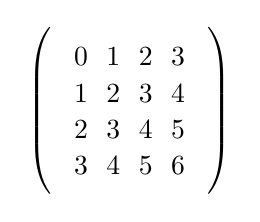
\begin{tikzpicture}
        \matrix [matrix of math nodes,left delimiter=(,right delimiter=)] (m)
        {
            0 & 1 & 2 & 3 \\
            1 & 2 & 3 & 4 \\
            2 & 3 & 4 & 5 \\
            3 & 4 & 5 & 6 \\
        };  
    \end{tikzpicture}
\end{center}
We want all jobs to have a different ID. We redefine the job\_ID to be
\begin{equation}
job\_ID = i \times N + j .
\end{equation}
Using this definition our matrix of job\_IDs becomes
\begin{center}
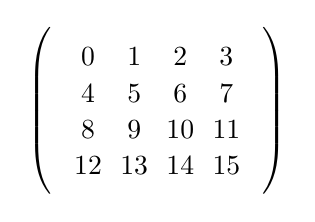
\begin{tikzpicture}
        \matrix [matrix of math nodes,left delimiter=(,right delimiter=)] (m)
        {
            0 & 1 & 2 & 3 \\
            4 & 5 & 6 & 7 \\
            8 & 9 & 10 & 11 \\
            12 & 13 & 14 & 15 \\
        };  
    \end{tikzpicture}
\end{center}
Each matrix element represent a job\_ID. Here each job has got its
unique ID, and it is easier to distribute. When we distribute work we
must use the MPI rank and total number of MPI processes $p$. For example we
can define a condition for each processor that must be true if the
processors are to perform the job
\begin{lstlisting}
if (job_ID % p = rank){
   // Perform job
}
\end{lstlisting}
From the perspective of our CPUs we can use this relation to identify
our job distribution. Noted now in the matrix is what processor
performs which job. We assume we have $p = 8$, 
\begin{center}
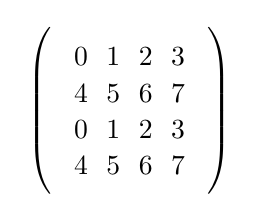
\begin{tikzpicture}

        \matrix [matrix of math nodes,left delimiter=(,right delimiter=)] (m)
        {
            0 & 1 & 2 & 3 \\
            4 & 5 & 6 & 7 \\
            0 & 1 & 2 & 3 \\
            4 & 5 & 6 & 7 \\
        };  
    \end{tikzpicture}
\end{center}
We see the job distribution is optimal, because the amount of work for all CPUs are identical. If we used the job\_ID defined in Eq. \eqref{example_job_distribution} the amount of work for each processor would not be the same. This is a sub-optimal work distribution. 

\subsection{Why Parallel}
Constructing a parallel program seems like quite the challenging
feature. Every year there are new processors released with improved
performance. Why do we not just wait for a great CPU that can solve
all our problems? The reason we do not wait for this, is that it will
never happen. The problem with great performance CPUs is that their
power consumption is generally very high. A CPU with twice the
performance generally needs 3 or 4 times the power, according to a
lecture from Intel on parallel programming,
\cite{intelduden_citeation}. It is therefore much more feasable to
have several CPUs with less performance, than one high performance
CPU. \\

So not only does parallel programming enable us to perform
calculations faster and on larger systems, it also requires less
power. Power consumption is the limiting factor in CPU performance
today. Parallel programming is thus very important, and likely to
become even more important in the future. On a sidenote, this is a
reason why GPUs have become so popular, GPUs are optimized for
performance per watt. Christoffer Hirth wrote extensively about this
in his thesis, \cite{non_refer_numba1}. His principles has not been
incorporated in our implementation, but is a likely source of further
performance gains.

\section{OpenMP}
OpenMP is another library for parallel programming. It is developed by
Intel and can be activated in most compilers. OpenMP uses shared memory
model. Here the main memory is available on all processors. The key
word here is main memory, as each processor has its own cache. OpenMP
is very easy to get started with. We will not be using it, but more
information is available in for example Ref.~\cite{openmp_citation_po_g}.

\section{External Math Libraries}
External Math Libraries are optimized for performance. They have
built-in functions to handle matrix-matrix multiplications,
vector-matrix multiplications, and similar problems. The best
libraries are the likes of OpenBLAS, \cite{openblas_citation}, and
Intel MKL, \cite{mkl_citation}. For our implementation we will make
use of MKL on the Abel computing cluster. These libraries often give a
huge performance gain in matrix operations, relative to a naive
for-loop implementation. \\

We also mention that MKL comes with a parallel version, where it
makes use of OpenMP. Both these libraries are developed by Intel. For
our purposes we only made use of the serial version.











\chapter{Implementation}
In this chapter we will discuss the implementation of all methods
discussed in the previous chapters. We will implement them all in one
program. We want to give our program a few positive features. First,
we want people who know nothing about programming to be able to make
use of our program. A background in chemistry is ideal for making use
of quantum chemistry methods. However, a background in chemistry does
not always include programming. For this reason, we encourage the
chemistry community to look into the complete package presented in
this chapter. Second, we want it to be effective, and go in
parallel. \\

This chapter is divided into six sections. First we look at how a
program user can give input and run the program. Next we examine the
general structure. The following four sections discuss the details of
HF, AOtoMO, serial CCSD and parallel implementation of CCSD. All
ideas, code and wise remarks in this chapter are written
from scratch by the author. The implementation is of course not the
only one possible, for this reason we also include some citations to
alternative implementations were appropriate.

\section{Input File}
This section will deal with the user friendly part of our
program. This means easy input. We must be able to define what method
to use, what atoms and where they are placed and other input
variables. We want these to be defined in a separate textfile, to
ensure the user never needs to recompile or edit any code. The input
file must be named "INCAR". \\

\begin{figure}[h!]
\begin{center}
\fbox{\includegraphics[width=\textwidth]{inputfile100.eps}}
\caption{Example of input file for our program}
\label{fig:inputfile100}
\end{center}
\end{figure}

An example of an input file is given in figure
\ref{fig:inputfile100}. This is the only file we need in order to change the
system or method in use. Our program uses the standard fstream library
to read the textfile. We then go through it searching for
keywords. The keywords are defined to be the leftmost word in each
line. \\

Basis\_Set is the first keyword. Here we can choose from a variety of
basis sets and the program will make use of this. The current options
are STO-3G, 3-21G, 4-31G, 6-31G, 6-311ss, 6-311-2d2p and
6-311-3d3p. Most of basis sets are implemented for all atoms for which
they are available. \\

The next keyword is Method. Here the choices are HF, CCSD, CCSDT-1a, CCSDT-1b, CCSDT-2, CCSDT-3, CCSDT-4 and CCSDT. The CCSDT part will be discussed in the next chapter. \\

The quantity convergence\_criteria is defined to be $10^{n}$, where n
is given in the textfile. As an example, $-8.0$ gives a convergence
criteria of $10^{-8}$. The same convergence criteria is used for all
methods. \\ The variable Relax\_Pos is meant to call a relaxation
procedure, but this is not implemented in this version of the
program. \\ The quantity use\_angstrom gives the user the option to
give atomic coordinates in angstrom, instead of atomic units. The
options here are true or false. If it is set to true the coordinates
are transformed to atomic units inside the program. \\

print\_stuffies is a variable that gives the user the option if he/she
wants extra values printed. If this is set to true there are several
interesting numbers printed during calculations. If this is set to
false we only print the final energy. This option is added for a
situation where we want to perform several hundred smaller
calculation. 
Freeze\_Core is an option available for CCSD. This will freeze the core electrons. \\

The next few lines give the atoms and their positions. The first
letter is used to determine the number of electrons and the charge of the nucleus or nuclei.
The program does not deal with ions. 

The input file stops searching for keywords once they are all
found. Hence the user is free to put comments in the input
file, as long as they are not placed next to keywords or inside the
ATOMS section.

\section{General Code Overview}
In this section we describe the general overview of the code. We will
present this in terms figures, and fill in the blanks throughout the
remaining sections. Each class will be described by its input, output
and internal workings. \\

\begin{figure}[h!]
\begin{center}
\fbox{\includegraphics[width=\textwidth]{structure.eps}}
\caption{Code structure}
\label{fig:structure}
\end{center}
\end{figure}

The first class to report for duty is the initializer. This class
takes the input from main and makes sure we use it correctly. If
angstroms is used as units, the coordinates are transformed to atomic
units. If we want extra print options, this is ensured here. We also
define a Hartree Fock object in this class, since all methods in
computational chemistry generally start with a HF calculation. \\

We then make sure the correct method is called, and pass this
object. For this reason we drew an arrow from HF to initializer only
in figure \ref{fig:structure}, since it is now passed as input to the
other methods.


\section{Hartree Fock}
In this section we discuss the HF implementation in detail. Our
Hartree Fock implementation is grounded in the class
hartree\_fock\_solver. The main function is called Get\_Energy. In
this function we will calculate the HF energy. The main outlay can be
seen in figure \ref{fig:hfimp}. \\

\begin{figure}[h!]
\begin{center}
\fbox{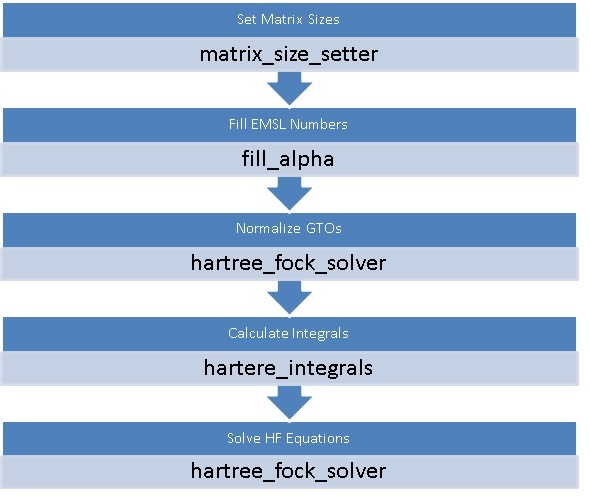
\includegraphics[width=\textwidth]{hf_imp.jpg}}
\caption{Basic Outlay of HF Implementation. First column is what action is done, second column is in what class this action takes place}
\label{fig:hfimp}
\end{center}
\end{figure}

The code is described in the text. We have also included key lines
from the code itself to better illustrate the implementation. \\

\subsubsection{Filling numbers from EMSL}
\begin{lstlisting}
   // Set Matrix Sizes
   matrix_size_setter matset(Z, Basis_Set, n_Nuclei);
   Matrix_Size = matset.Set_Matrix_Size();

   // Fill numbers from EMSL
   Fill_Alpha Fyll(n_Nuclei, Z, Basis_Set,
Matrix_Size, matset.Return_Max_Bas_Func());
   alpha = Fyll.Fyll_Opp_Alpha();
   c = Fyll.Fyll_Opp_c();
   n_Basis = Fyll.Fyll_Opp_Nr_Basis_Functions();
   Number_Of_Orbitals = Fyll.Fyll_Opp_Antall_Orbitaler();
   Potenser = Fyll.Fyll_Opp_Potenser();
\end{lstlisting}

The first procedure performed in this function is to call the
matrix\_size\_setter class. We make an object of this class and send
the basis set in use and which atoms are in play. This class then
returns how large our arrays must be. We then allocate these
arrays. \\

The next step is going to the fill\_alpha class. This class contains
data from EMSL, and fills up this data in arrays. The array alpha is
filled with values for $\alpha_i$, the array c is filled with values
of $c_i$. We also
make a one dimensional array, Number\_Of\_Orbitals, which holds
information on how many basis functions are in use for a specific
atom. The array n\_Basis holds how many primitives each of these
consist of. \\

\subsubsection{Normalizing GTOs}
\begin{lstlisting}
   // Normalize coefficients from EMSL
   Normalize_small_c();
\end{lstlisting}

The next step is to multiply in the normalization constant. This is
multiplied in with the array c, through the function
Normalize\_small\_c. In this function we have implemented the
equations from section \ref{normalization_section}. \\

\subsubsection{Overlap Integrals}
The next step is to make an object of the class
hartree\_integrals. Inside this class we will eventually calculate all
the integrals we need. However the first step is to fill up an array
of $E_t^{ij}$. These values are present in all our integrals. For this
we use Eqs. \eqref{important_hf1}, \eqref{important_hf2} and
\eqref{important_hf3}. The values for $E_t^{ij}$ will be calculated
for all combinations of two primitive GTOS. This enables us to reuse
the values in all our integrals, even the electron-electron
repulsion. \\

\begin{lstlisting}
   // Precalculations
   HartInt.Fill_E_ij();

   // Overlap
   O = HartInt.Overlap_Matrix();
\end{lstlisting}

We then calculate the integrals. The overlap is stored in a matrix $S$
and is calculated using Eq. \eqref{overlap_integral}. \\

\subsubsection{Kinetic Energy}
The two index integrals are stored in a matrix EK. EK consists of our
kinetic energy and the nucleus-electron interaction. \\

\begin{lstlisting}
   // One electron operator
   EK = -0.5*HartInt.Kinetic_Energy()+
   - HartInt.Nuclei_Electron_Interaction();
\end{lstlisting}

The kinetic energy is calculated using Eq. \eqref{EKintegralsss}. \\

\subsubsection{Hermite Integrals}
For the nucleus-electron interaction we need to calculate the Hermite
Integrals, $R_tuv^n$. We make a new function to calculate these called
Set\_R\_ijk. This function implements the equations given in
Eqs. \eqref{nucelec_0_int}, \eqref{nucelec_1_int},
\eqref{nucelec_2_int} and \eqref{nucelec_3_int}. We include the
implementation of Eqs. \eqref{nucelec_0_int} and
\eqref{nucelec_1_int}. We put the values in a global four dimensional
array R\_ijk.

\begin{lstlisting}
void Hartree_Integrals::Set_R_ijk(double p, int t, int u, int v, rowvec R1, rowvec R2)
{
   int t_max,nn,i,j,k,tt = t,uu = u,vv = v;
   t_max = t+u+v;
   double Boys_arg;
   rowvec Rcp(3);
   Rcp = R1-R2;
   Boys_arg = p*dot(Rcp, Rcp);
   Boys_arg = Boys(Boys_arg, 0);
   
   // Initialize R^n_0,0,0
   for (nn=0; nn<(t_max+1);nn++){
      R_ijk.at(nn)(0,0,0) = pow(-2*p, nn) *    F_Boys(nn);
   }

   // Fill up R^n_i,0,0
   for (i=0; i<tt; i++){
      for (nn=0; nn<(t_max-i); nn++){
         R_ijk.at(nn)(i+1,0,0) = Rcp(0) * R_ijk.at(nn+1)(i,0,0);
         if (i > 0){
            R_ijk.at(nn)(i+1,0,0) += i * R_ijk.at(nn+1)(i-1,0,0);
         }
      }
   }
   
   // Rest of Set_R_ijk function   
\end{lstlisting}
We here make use of the Boys function.

\subsubsection{Boys Function}
The function that calculates a value for the Boys function is called
Boys. We have two equations we can use, Eq. \eqref{boys_int_1} and
Eq. \eqref{boys_int_2}. One works for small values of $x$, the other for large
values of $x$. We define everything less than $x = 50$ to be small, and everything
greater or equal to 50 to be large. We include the implementation of
large $x$. \\

\begin{lstlisting}
if (x > 50){
   Set_Boys_Start(N);
   F = Boys_Start / pow(2.0, N+1) * sqrt(M_PI/pow(x, 2*N+1));
}
\end{lstlisting}
For small $x$ we Taylor expand around zero. We choose $M = 100$ in Eq. \eqref{boys_int_1} for the Taylor expansion. 

\begin{lstlisting}
else{
   double F=0, sum=0;
   int M;
   for (int j=0; j<100; j++){
      sum = pow(2*x, j);
      M = 2*N+1;
      while (M < (2*N+2+2*j)){
         sum /= M;
         M += 2;
      }
      F += sum;
   }
   F *= exp(-x);
}
\end{lstlisting}
We then use the recursive relation in Eq. \eqref{boys_int_3}. 

\begin{lstlisting}
F_Boys(N) = F;
for (int i = N; i > 0; i--){
   F_Boys(i-1) = (2*x*F_Boys(i) + exp(-x))/(2*i-1);
}
\end{lstlisting}
We are left with designing a value for $N$ where $N$ denotes the
starting $F_n$ value, from which we will iterate down to the
approximate solution. Popular here is putting $N$ as some function of
angular momentum, like $N = 6 \times l$. However we just put it to
30. In this value we were able to recreate all the benchmark values in
\cite{boys_referanse_1} and \cite{boys_referanse_2}. These articles
discuss the numerical calculation of the Boys function.

\subsubsection{Nucleus-Electron Interaction}
With these functions we can implement nucleus-electron interaction as
given in Eq. \eqref{final_nuclei_electron_thang}. We add these into
the array EK.

\subsubsection{Electron-Electron Interaction}
The electron-electron repulsion integrals are stored in a four
dimensional field, field\_Q. They are calculated through a function
called Calc\_Integrals\_On\_The\_Fly. This function takes the input of
four orbitals, i, j, k, l, and returns its value for $\langle i j | k
l \rangle$. The function is an implementation of
Eq. \eqref{electron_electron_int_1_1}, also using
Eq. \eqref{electron_electron_int_1_2}. \\

\begin{lstlisting}
double Calc_Integrals_On_The_Fly(int orb1, int orb2, int orb3, int orb4)
{    
    int i,j,k,m;

    // Figure out what atom the AO belongs to, need atomic position
    i = Calc_Which_Atom_We_Are_Dealing_With(orb1);
    j = Calc_Which_Atom_We_Are_Dealing_With(orb3);
    k = Calc_Which_Atom_We_Are_Dealing_With(orb2);
    m = Calc_Which_Atom_We_Are_Dealing_With(orb4);

    // Here we calculate the two electron integrals
    // We have already stored E_ij^t so we reuse these
    // Symmetry considerations are applied elsewhere.

    int E_counter1, E_counter2; // These ensures we get the right E_ij^t
    int n,p,o,q; // Index for primitive GTO
    double temp = 0;
    E_counter1 = E_index(orb1,orb2);
    for (n=0; n<n_Basis(orb1); n++)
    {
        for (p=0; p<n_Basis(orb2); p++)
        {
            E_counter2 = E_index(orb3, orb4);
            for (o=0; o<n_Basis(orb3); o++)
            {
                for (q=0; q<n_Basis(orb4); q++)
                {
                    temp += c(orb1,n)*c(orb2,p)*c(orb3,o)*c(orb4,q)*
                            HartInt.Electron_Electron_Interaction_Single
                (orb1, orb3, orb2, orb4,
                  i, j, k, m, n, o, p,
                q, E_counter1, E_counter2);

                // E_t^ij is stored for x,y,z direction
            // Hence +3 on the counter
                    E_counter2 += 3;
                }
            }
            E_counter1 += 3;
        }
    }
    return temp; // temp is the value of <ij|kl>
}
\end{lstlisting}



We also take advantage of the eighfold symmetries, written our in
Eqs. \eqref{interchangesym} and \eqref{interchangesym2}. We
constructed the code like this originally to have the option to not
store these integrals at all, and instead calculate them as
needed. This would be a game changer in terms of what calculations are
possible, since memory would now be scaling as $n^2$ instead of
$n^4$. However we later decided that a memory distribution model was
sufficient for our purposes, since we want to use coupled
cluster theory after our Hartree-Fock calculations. 
Coupled Cluster theory use more memory than HF, posing thereby complicated challenges to the available memory.

\subsubsection{Parallel Implementation and Memory Distribution}
The hotspot in the HF solver is the two electron integrals. We are not looking to
make an optimized HF solver, but we must run this part of the
calculation in parallel. \\

We want the workload of the integrals $\langle i j | k l \rangle$
distributed for a given index $i$ and $j$. We only calculate one version
of each symmetric term. \\

\begin{lstlisting}
    field_Q.set_size(Matrix_Size, Matrix_Size);
    for (int i = 0; i < Matrix_Size; i++)
    {
        for (int j = 0; j < Matrix_Size; j++)
        {
        // Leave parts of the field un-initialized
        // size = number of MPI procs
        // rank = my MPI rank
            if ((i+j)%size == rank)
            {
                field_Q(i,j) = zeros(Matrix_Size, Matrix_Size);
            }
        }
    }
\end{lstlisting}

The two electron integrals are a part of the Fock matrix calculation. We want to run this also in parallel, so ensure we can keep the integrals distributed in memory. We remember the Fock matrix was dependant upon 

\begin{equation}
\sum_{kl} \langle i j | k l \rangle ,
\end{equation}
and

\begin{equation}
\sum_{kl} \langle i l | k j \rangle .
\end{equation}
Because of this we define field\_Q to store the integrals as such

\begin{equation}
field\_Q(i,k)(j,l) = \langle i j | k l \rangle .
\end{equation}
We place the two indexes to be swapped in the matrix part of our armadillo field. We then store a $N^3$ sized array of temporary values, F\_temp(i,j,k). We then add the terms together in the correct order to produce $F_{ij}$. Here we can use functions like MPI\_Reduce, or make our own implementation of this function to produce the same result. \\

The important feature is that each processor only calculates terms
based on the indices $i$ and $k$. This enables us to leave the indices not
in use in the field undefined, thus distributing the $N^4$ memory over
all our $P$ MPI processors in use ( dubbed MPI procs hereafter). Each processor then only
stores $\frac{N^4}{P}$ doubles. The amount of bytes for communication
scales as $N^3$ doubles. \\

However, earlier we calculated the integrals with a work distribution
of indices $i$ and $j$. This work distribution makes it easier to use
symmetries to avoid recalculations of symmetric terms. We therefore
also introduce a communication procedure where we reshuffle the terms
in field\_Q among the MPI procs. The amount of bytes for communication
here is $\frac{1}{8} N^4$, and must be done using MPI\_Alltoallw or a
similar implementation producing an identical result. Our HF
implementation is not particularly optimized. Comments on how we could
optimize this implementation is available in the Conclusions chapter.

\subsubsection{Pre Iterative Steps}
The equation to solve in HF is the eigenvalue equation from
Eq. \eqref{FOCK_EQUATION_STUFF}. To do this on a computer we must
rewrite it slightly. The equation stands as

\begin{equation}
F C = S C \epsilon . \label{fdsaghbxcxd}
\end{equation}
We define a matrix $V$ that satisfies

\begin{equation}
V^{\dag} S V = I , \label{fdsafafdsafdsafa}
\end{equation}
where $I$ is the identity matrix. We insert $V^{\dag}$ to the left on both sides. Also $V V^{-1} $ is inserted into the equations. This leaves
\begin{equation}
V^{\dag} F V V^{-1} C = V^{\dag} S V V^{-1} C \epsilon .
\end{equation}
We also define 

\begin{equation}
F' = V^{\dag} F V ,
\end{equation}
and

\begin{equation}
C' = V^{-1} C .
\end{equation} 
We insert Eq. \eqref{fdsafafdsafdsafa}, $F'$ and $C'$ into Eq. \eqref{fdsaghbxcxd} and have
\begin{equation}
F' C' = C' \epsilon .
\end{equation}
This is a true eigenvalue problem, where $\epsilon$ will be the eigenvalues of $F'$ and $C'$ will be the corresponding 
eigenfunctions. \\

We also define an intermediate $P$, which will be the electron density as
\begin{equation}
P_{ij} = \sum_k^N C_i^k C_j^k ,
\end{equation}
where $N$ is the number of electrons. We are now ready to begin an iterative procedure. This procedure will be different for restricted HF (RHF) and  unrestricted HF ( UHF). 

\subsubsection{RHF Iterative Procedure}
Initially we put the density $P$ to be filled with zeroes. In RHF we
will have an equal number of electrons with spin up and spin
down. This simplifies our density matrix to

\begin{equation}
P_{ij} = \sum_k^{N/2} C_i^k C_j^k .
\end{equation}
We use Eq. \eqref{Fock_Restricted_1} to find the Fock matrix. We first insert $P$ into the equation and get
\begin{equation}
F_{ij} = (EK)_{ij} + \sum_{kl} P_{kl} (2 \langle i j | k l \rangle - \langle i l | k j \rangle) .
\end{equation}
We then perform the iterations until we reach self consistency. \\

\begin{algorithm}[H]
 \While{RHF\_continue = true}{
  Calculate $F$ \\
  $F' = V^{\dag} F V$ \\
  Solve $F' C' = C' \epsilon$ \\
  Compute $C = V C'$ \\
  Compute P \\
  \If{RHF = converged}{
    RHF\_continue = false
  }
 }
 \caption{Psudocode for RHF iterations}
 \label{RHF_ITERATIVE_PROCEDURE}
\end{algorithm}
After we have reached self consistency we calculate the energy.

\begin{lstlisting}
double Hartree_Fock_Solver::Calc_Energy()
{
    // Optimized RHF energy calculations
    Single_E_Energy = accu(EK % P);
    Two_E_Energy = 0.5*accu(Energy_Fock_Matrix % P) - 0.5*Single_E_Energy;
    return Single_E_Energy+Two_E_Energy;
}
\end{lstlisting}
Using armadillo the energy calculation simplifies to only two lines of code. 

\subsubsection{UHF Iterative Procedure}
For UHF we define two densities, $P^{\alpha}$ and $P^{\beta}$, which are the densities for spin up and down
\begin{equation}
P^{\alpha}_{ij} = \sum_k^{N_{\alpha}} C^{\alpha}_{ik} C^{\alpha}_{jk},
\end{equation}
and
\begin{equation}
P^{\beta}_{ij} = \sum_k^{N_{\beta}} C^{\beta}_{ik} C^{\beta}_{jk} .
\end{equation}
Here $N_{\alpha}$ is the number of spin up particles, while
$N_{\beta}$ is the number of spin down particles. These must be
defined as input as must be equal to the total number of electrons in
the system. We define the starting density to be random uniform
numbers. We ensure the two matrices are not equal to each other for
the first iteration. We use Eqs. \eqref{Fock_Restricted_2} and
\eqref{Fock_Restricted_3} to find the Fock matrices. \\

\begin{algorithm}[H]
 \While{UHF\_continue = true}{
  Calculate $F_{\alpha}$ \\
  Calculate $F_{\beta}$ \\
  $F_{\alpha}' = V^{\dag} F_{\alpha} V$ \\
  $F_{\beta}' = V^{\dag} F_{\beta} V$ \\
  Solve $F_{\alpha}' C_{\alpha}' = C_{\alpha}' \epsilon_{\alpha}$ \\
  Solve $F_{\beta}' C_{\beta}' = C_{\beta}' \epsilon_{\beta}$ \\
  Compute $C_{\alpha} = V C_{\alpha}'$ \\
  Compute $C_{\beta} = V C_{\beta}'$ \\
  Compute $P_{\alpha}$ \\
  Compute $P_{\beta}$ \\
  \If{UHF = converged}{
    UHF\_continue = false
  }
 }
 \caption{Psudocode for UHF iterations}
 \label{UHF_ITERATIVE_PROCEDURE}
\end{algorithm}
After iterations we again calculate the energy. With armadillo the
energy calculation simplifies to just two lines of code.

\begin{lstlisting}
double Hartree_Fock_Solver::Unrestricted_Energy()
{
    // Oprimized energy for UHF
    Single_E_Energy = accu((P_up + P_down) % EK);
    Two_E_Energy = 0.5 * accu(EnF_up % P_up) + 0.5 * accu(EnF_down % P_down) - 0.5 * Single_E_Energy;
    return Single_E_Energy + Two_E_Energy;
}
\end{lstlisting}


\subsubsection{Helping Convergence}
Sometimes our solution has problems converging. This is a numerical
problem and we can introduce a few features to help the convergence
along. \\

Damping is one option. This means updating the density only slightly, by inserting

\begin{equation}
P_{new}' = \gamma P_{old} + \left( 1 - \gamma \right) P_{new} .
\end{equation}
This reduces the change in density between iterations. We only used this in UHF. \\

A better alternative is the DIIS method, discussed in section
\ref{diis_section_po_g}. We implemented this method for RHF. The first
part of our DIIS implementation is calculating the error, $\Delta p$
\begin{lstlisting}
delta_p = F*P*O - O*P*F;
\end{lstlisting}

We then store the error and Fock matrices for the last $M$ iterations. Here $M$ is defined to be $M = 3$ in our implementation. After this we construct the matrix $B$. 

\begin{lstlisting}
for (int i = 0; i < number_elements_DIIS; i++){
   for (int j = 0; j < number_elements_DIIS; j++){
      mat1 = Stored_Error.at(i);
      mat2 = Stored_Error.at(j);
      DIIS_B(i,j) = trace(mat1.t() * mat2);
   }
}
\end{lstlisting}

We then find the coefficients $c$.
\begin{lstlisting}
DIIS_c = solve(DIIS_B, DIIS_Z);
\end{lstlisting}

And finally we construct the new Fock matrix, as a linear combination of the previous Fock matrices. 

\begin{lstlisting}
F = DIIS_c.at(0) * Stored_F.at(0);
for (int i = 1; i < number_elements_DIIS; i++){
   F += DIIS_c.at(i) * Stored_F.at(i);
}
\end{lstlisting}

\section{Atomic Orbital to Molecular Orbital}
The transformation of Atomic Orbital (AO) to Molecular Orbital (MO) is
required before we can do any CCSD calculations. In this section we
describe how to implement this transformation. We are here looking for
a highly optimized implementation. Some background is available in
\cite{aotomo_1_cite}. However the author found the algorithms in the
literature unsatisfactory. For this reason we will present a new
algorithm. First, the simplest transformation is:

\begin{equation}
\langle ab | cd \rangle = \sum_{ijkl} C_i^a C_j^b C_k^c C_l^d \langle ij|kl \rangle .
\end{equation}
This scales as $n^8$ and can be factorized, namely
\begin{equation}
\langle ab | cd \rangle = \sum_i C_i^a \sum_j C_j^b \sum_k C_k^c \sum_l C_l^d  \langle ij|kl \rangle .
\end{equation}
This is usually split into four transformations, 

\begin{equation}
\langle aj|kl \rangle = \sum_{i} C_i^a \langle ij|kl \rangle ,
\end{equation}

\begin{equation}
\langle ab|kl \rangle = \sum_{j} C_j^b \langle aj|kl \rangle,
\end{equation}

\begin{equation}
\langle ab|cl \rangle = \sum_{k} C_k^c \langle ab|kl \rangle ,
\end{equation}
and
\begin{equation}
\langle ab|cd \rangle = \sum_{l} C_l^d \langle ab|cl \rangle .
\end{equation}
Each of these transformations scales as $n^5$. The implementation of
this must be done in an effective way in terms of speed and
memory. The latter is the most important as the memory here scales as
$N^4$, where N is the number of contracted GTOs, for both $\langle ij
| kl\rangle$, $\langle ab | cd \rangle$ and also the intermediates in
between each quarter transformation. \\

\begin{algorithm}[H]
 \KwData{Psudo Code}
 \KwResult{Algorithm for parallel AOtoMO transformation }
 \For{a=0; a<N}{
  \For{k=0; k<N}{
   \For{l=0; l<N}{
    \If{Grid k and l over threads}{
     \For{j=0; j<N}{
      \For{i=0; i<N}{
       $QT1(k,l,j) += 
       C_i^a \times \langle ij|kl \rangle$
      }
     }
     \For{j=0; j<N}{
      \For{b=0; b<N}{
       $QT2(k,l,b) += C_j^b \times QT1(k,l,j)$
       }
      }
    }
   }
  }
  Communicate $QT2(k,l,b)$
  
  \For{b=0; b<N}{
   \For{c=0; c<N}{
    \If{Grid b and c over threads}{
     \For{k=0; k<N}{
      \For{l=0; l<N}{  
       $QT3(b,c,l) = C_k^c \times QT2(k,l,b)$
       }
      }
      \For{l=0; l<N}{
        \For{d=0; d<N}{
       $QT4(b,c,d) = C_l^d \times QT3(b,c,l)$
        }
      }
     }
    }
   }
   
   Communicate $QT4(b,c,d)$\\
   
   \If{Store distributed MOs to given thread}{
    $\langle ab|cd \rangle = QT4(b,c,d)$
   }
 }
  
 \caption{Simple Psudocode for parallel AOtoMO transformation. QT1, QT2, QT3 and QT4 are intermediates}
 \label{aotomotrans}
\end{algorithm}

Algorithm \ref{aotomotrans} is a description of how we optimize this
implementation. Further optimizations will come later, but first an
illustration of the general idea. We first hold index $a$ constant
throughout the transformation. This enables us to use $N^3$ size
intermediates. \\

Second the grid over $k$ and $l$ is chosen because neither of these are
involved as an index in $C$ for the first two quarter
transformations. This makes sure that the terms of $QT2(k,l,b)$
calculated by each thread is the fully two quarter transformed
term. This avoids the use of MPI\_Reduce or similar operations and
means only one thread needs to communicate these two quarter
transformed terms with specific $k$ and $l$, minimizing the
communication. The total amount of double precision values
communicated in the first communication for now is $N^3$ for each $a$,
making it $N^4$ in total for all $a$. \\

After the first communication each thread has all terms in
$QT2(k,l,b)$ available. We then make a new grid over $b$ and $c$ and
continue calculations in parallel. The grid could be made over $a$ and
$b$, but the prior makes in general a better work distribution. This
is because index $a$ is held fixed. After the fourth quarter
transformation each thread has the fully transformed MOs available for
certain $b$ and $c$ indexes. \\

At this point we can distribute the MOs in the same grid as for $b$
and $c$, and start CCSD calculations. However because we want to have
the distribution optimized for CCSD we implement another
communication. This communication is $N^3$ for each $a$, making it
$N^4$ in total for all $a$. \\

After the second communication we simply store the MOs in a memory
distributed manner. It is also possible to write to disk. \\

The quantities $QT2$ and $QT4$ must be stored as one dimensional
arrays, to minimize the number of communication procedures initiated,
hence minimize latency. Also all multiplications are written using
external math libraries through armadillo. We should also introduce
symmetries to optimize our calculations further. The starting AOs had
eight-fold symmetries. So does the resulting MOs. However these
symmetries do not hold at all the quarter transformed
intermediates. This complicates things slightly. \\

However we are in luck. The second quarter transformed four
dimensional array, QT2, will have symmetries in the two untouched
indexes, as well as in the two transformed indexes. We were able to
make use of this to reduce communication by 75\%, since symmetric
terms need not be communicated twice. This also holds true at the QT4
level obviously. The algorithm using symmetries and external math
libraries is presented in algorithm \ref{aotomo2}. \\

\begin{algorithm}
 \KwData{Psudo Code}
 \KwResult{Effective Algorithm for parallel AOtoMO transformation using external math libraries}
 \For{a=0; a<N}{
  \For{k=0; k<N}{
   \For{l=0; l<=k}{
    \If{Calculate on local thread}{
     A1(*) = C(a,*) $\times$ $\langle kl | ** \rangle$ \\
     A2($0 \rightarrow a$) = C($0 \rightarrow a$, *) $\times$ A1 \\
     \For{b=0; b<=a}{
       QT2(b,k,l) = A2(b) 
      }
    }
   }
  }
  
  MPI\_Allgatherv(QT2) \\
  
  \For{b=0; b<=a}{
   \For{c=0; c<N}{
    \If{Calculate on local thread}{
 	 A1(*) = C(c,*) $\times$
 	  QT2(b,*,*) \\
     A2($0 \rightarrow c$) = C($0 \rightarrow c$, *) $\times$ A1 \\
     \For{d=0; d<=c}{
       QT4(b,c,d) = A2(d) 
      }
     }
    }
   }
   MPI\_Allgatherv(QT4) \\
   
   \If{Store distributed MOs to given thread}{
    $\langle ab|cd \rangle = QT4(b,c,d)$ \\
    or write to disk
   }
 }
  
 \caption{Psudocode for parallel AO to MO transformation using armadillo. A1 and A2 are one dimensional intermediates}
 \label{aotomo2}
\end{algorithm}

The communication is somewhat tricky in this algorithm. Since we have
inserted symmetries, the size of the message to be transmitted changes
dependant upon the index $a$. This also applies to the
displacement. We therefore store both in two dimensional arrays where
$a$ is the outer index, the inner is the MPI rank. \\

We run through the algorithm one time in advance to calculate these
variables. We also calculate and store where each processor will start
calculations. This is done to remove any pipeline flushes, which can
be caused by the CPU wrongly guessing the answer of an if test. \\

For this reason we define another two dimensional array, this one of
size $N$ times the number of MPI procs. In the first two quarter
transformation, each rank here stored at what index $l$ will
calculations start for a given index $k$. The next $l$ the same rank
will perform calculations on will then be

\begin{equation}
l \rightarrow l + p
\end{equation}
where $p$ is the number of MPI procs. The exact same procedure is repeated for quarter transformation 3 and 4. \\

We have also in the more advanced algorithm inserted one dimensional
arrays A1 and A2. Using these provide more optimize ways of accessing
memory. It may at first sight seem like an additional complication to
first calculate A2 as a one dimensional array and later store it in
QT2, but this is a more efficient way when using armadillo. \\

The algorithm is implemented in the function 

\begin{lstlisting}
void Prepear_AOs(int nr_freeze);
\end{lstlisting}
The argument is how many core orbitals to freeze. 

\section{CCSD Serial Implementation \label{optimize_serial_version_bii}}
Our CCSD implementation is quite large, actually close to 10 000
lines. However this is small compared to other optimized
implementations, which are usually around 40 000 lines of
code. Implementation is important in CCSD, since it scales quickly for
larger systems. Additional information on the advancement of CCSD
is available in a series of books and articles,
\cite{book_om_advancements_ccsd}. The most effective implementation to
the authors knowledge is the Cyclic Tensor Framework, see
\cite{most_effective_ccsd_dude}, \cite{most_effective_ccsd_dude2} and
\cite{most_effective_ccsd_dude3}. \\

In this thesis we will present a simple and effective implementation
of CCSD in parallel. First we look at a simple serial
implementation. This section discusses the serial
implementation. There are two specific goals for this
implementation. First getting the energy in the smallest amount of
time, second being able to run larger systems. \\

Even more precise we can state that our goals are: \\
a) Never get zero in a multiplication\\
b) All multiplications should be done by external math libraries\\
c) Do not store anything more than needed\\

We first present the general structure of the code. Later we will
discuss a few details about different optimizations we have
implemented. These will be contrasted to what kind of optimizations is
commonly implemented in CCSD. Then, there will be a pros and cons list
for our implementation. The chapter will be quite technical as there
are several considerations behind each optimization, and they all work
in combination.

\subsection{Structure}

For our serial program we first define arrays to store all
intermediates, MOs and amplitudes. Two arrays are defined for each
amplitude, one for the old amplitudes and one for the new
amplitudes. We define a convergence criteria, which stops iterations
once the difference of energy from one iteration to the next is bellow
this criteria. \\

\begin{algorithm}[H]
 \KwData{Psudo Code}
 \KwResult{Structure of CCSD serial program}
 \While{CCSD continue = true}{
  Set Eold = Enew \\
  Calc F1 \\
  Calc F2 \\
  Calc F3 \\
  Calc W1 \\
  Calc W2 \\
  Calc W3 \\
  Calc W4 \\
  Calc New t1 amplitudes \\
  Calc New t2 amplitudes \\
  Set t1 = t1new \\
  Set t2 = t2new \\
  Calc $\tau_{ij}^{ab}$ \\
  Calc New Energy \\
  \If{Enew - Eold < Convergence criteria}{
  	CCSD continue = false
  }
 }
 \caption{Psudocode for our serial CCSD program}
 \label{CCSD_STRUCTURE_SERIAL}
\end{algorithm}

Algorithm \ref{CCSD_STRUCTURE_SERIAL} illustrates the algorithm as psudocode. Each of the terms behind "Calc" is taken as a separate function to make the code easily readable. 

\subsection{Removing redundant zeroes \label{compact_storage}}
We now briefly reconsider the molecular integrals, which were calculated as

\begin{equation}
\langle pq|rs \rangle = \sum_{\alpha \beta \xi \nu} C_{\alpha}^p
C_{\beta}^q C_{\xi}^r C_{\nu}^s \langle \alpha \beta | \xi \nu \rangle
.
\end{equation}
Here $\langle \alpha \beta | \xi \nu \rangle$ are our atomic orbitals
(AOs). These come from our RHF calculations. The quantities $\langle pq|rs \rangle$
are the molecular orbitals (MOs). MOs here are presented as a linear
combination of AOs. The MOs appear in CCSD as a double bar
integral. This is defined as 
\begin{equation}
\langle pq||rs \rangle = \langle pq | rs \rangle
- \langle pq | sr \rangle  .
\end{equation}
Due to spin considerations, if we fill a matrix with $\langle pq||rs
\rangle$ it will be filled with mostly zeroes. However when using an
RHF based CCSD it is common that all even numbered orbitals have the
same spin orientation. This means all odd numbered orbitals will also
have the same spin orientation. This results in the zeroes forming
pattern that we have identified and utilized. \\

The quantities $\langle pq || rs \rangle$ are diagonal in total spin
projection. In RHF the total spin is also equal to zero. When we have
all odd numbered orbitals with the same spin orientation, and same
with even numbered orbitals, this has a practical implication. The
implication is that the only terms that will not be equal to zero are
those where the sum of the orbital indices are equal to an even
number. \\

We will now visualize this. We construct a program that performs the
AO to MO transformation and print $\langle pq||rs \rangle$ for a fixed
$p=1$ and $r=1$. In the span of $q$ and $s$ there is formed a matrix,
we have noted the terms that will be zero and also the terms that will
be non-zero with the indices $(q, s)$.

\[ \left( \begin{array}{ccccccc}
(0,0) & 0 & (0,2) & 0 & (0,4) & 0 & \dots \\
0 & (1,1) & 0 & (1,3) & 0 & (1,5) & \dots \\
(2,0) & 0 & (2,2) & 0 & (2,4) & 0 & \dots \\
0 & (3,1) & 0 & (3,3) & 0 & (3,5) & \dots \\
(4,0) & 0 & (4,2) & 0 & (4,4) & 0 & \dots \\
0 & (5,1) & 0 & (5,3) & 0 & (5,5) & \dots \\
\dots & \dots & \dots & \dots & \dots & \dots & \dots \end{array} \right)\]

This array is now stored in our computer as a four dimensional array
that we call $I[a][b][c][d]$. We on purpose use a different kind of
indexing for our stored integrals, even though index $a$ in this
example is a referance to orbital $p$. We can note which orbitals our
array-indexes refers to as such\\ a = p \\ b = r \\ c = q \\ d = s \\

This will be an array of size $(2N)^4$, where $N$ is the number of contraction Gaussian Type Orbitals (GTOs). We now perform a trick. We want our indexes of I to refer to a different orbital, in practice we want:\\
a = p\\
b = r\\
c = q/2 + (q\% 2) N\\
d = s/2 + (s\% 2) N\\

Where \% is the binary operator and we use integer division by 2. Now,
index c is no longer a referance to orbital q, but a referance to
orbital [q/2 + (q \% 2) N]. If we now visualize the same double bar
integral with fixed $p=1$ and $r=1$ it looks like this

\[ \left( \begin{array}{cccccccc}
(0,0) & (0,2) & (0,4) & \dots & 0 & 0 & 0 & \dots \\
(2,0) & (2,2) & (2,4) & \dots & 0 & 0 & 0 & \dots\\
(4,0) & (4,2) & (4,4) & \dots & 0 & 0 & 0 & \dots\\
\dots & \dots & \dots & \dots & \dots & \dots & \dots & \dots\\
(1,1) & (1,3) & (1,5) & \dots & 0 & 0 & 0 & \dots\\
(3,1) & (3,3) & (3,5) & \dots & 0 & 0 & 0 & \dots\\
(5,1) & (5,3) & (5,5) & \dots & 0 & 0 & 0 & \dots\\
\dots & \dots & \dots & \dots & \dots & \dots & \dots & \dots \end{array} \right)\]

Performing this trick will always result in a matrix that looks something like this. We can split this matrix into four sub-matrices, one top left, one top right, one bottom left and one bottom right. Regardless of $a$ and $b$, we will always have either the two left sub-matrices, or the two right sub-matrices always filled with zeroes. These do not need to be stored. If we ensure we \emph{only perform calculations on orbitals with a non-zero contribution} we can change our array-indexing to:\\
a = p\\
b = r\\
c = q/2 + (q\% 2) N\\
d = s/2 \\

This means for two orbital where s = 2 and s = 3 we will have the same d value. However one of these orbitals will always be zero, so if we avoid doing calculations on this there will be no problems. And we also reduce the size of the array to half. Visualizing now the same array it looks like this.
\[ \left( \begin{array}{cccc}
(0,0) & (0,2) & (0,4) & \dots \\
(2,0) & (2,2) & (2,4) & \dots \\
(4,0) & (4,2) & (4,4) & \dots \\
\dots & \dots & \dots & \dots \\
(1,1) & (1,3) & (1,5) & \dots \\
(3,1) & (3,3) & (3,5) & \dots \\
(5,1) & (5,3) & (5,5) & \dots \\
\dots & \dots & \dots & \dots  \end{array} \right)\]

And its size will be $\frac{1}{2} (2N)^2$. This kind of indexing can and should be performed on $\textbf{all}$ stored integrals, amplitudes and intermediates. This ensures all memory is reduced by at least 50 \%. Also if a,b,c,d is referencing orbitals in the same manner in all stored arrays we can still use external math libraries as before. However now we will not be passing any zeroes into these external math libraries, so calculations can be faster. This change in indexing keeps all symmetries and also allow easy row and column access. The row is accessed as usual.

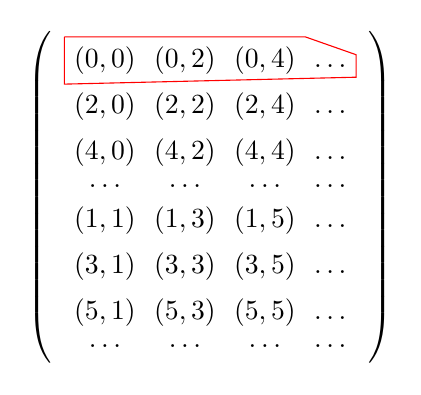
\begin{tikzpicture}
        \matrix [matrix of math nodes,left delimiter=(,right delimiter=)] (m)
        {
            (0,0) &(0,2) &(0,4) &\dots \\
            (2,0) & (2,2) & (2,4) & \dots \\
            (4,0) & (4,2) & (4,4) & \dots \\
            \dots & \dots & \dots & \dots \\
            (1,1) & (1,3) & (1,5) & \dots \\
			(3,1) & (3,3) & (3,5) & \dots \\
			(5,1) & (5,3) & (5,5) & \dots \\
			\dots & \dots & \dots & \dots \\
        };  
        \draw[color=red] (m-1-1.north west) -- (m-1-3.north east) -- (m-1-4.north east) -- (m-1-4.south east) -- (m-1-1.south west) -- (m-1-1.north west);
    \end{tikzpicture}

A column is slightly different, since we only require either the top half or the bottom half of the matrix.

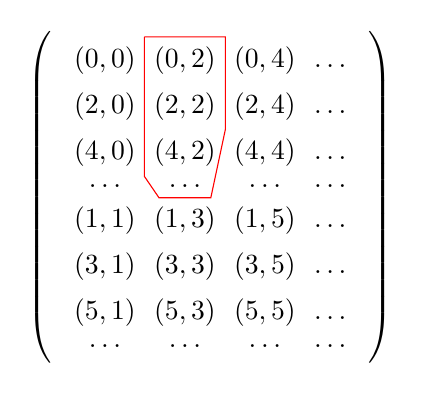
\begin{tikzpicture}
        \matrix [matrix of math nodes,left delimiter=(,right delimiter=)] (m)
        {
            (0,0) &(0,2) &(0,4) &\dots \\
            (2,0) & (2,2) & (2,4) & \dots \\
            (4,0) & (4,2) & (4,4) & \dots \\
            \dots & \dots & \dots & \dots \\
            (1,1) & (1,3) & (1,5) & \dots \\
			(3,1) & (3,3) & (3,5) & \dots \\
			(5,1) & (5,3) & (5,5) & \dots \\
			\dots & \dots & \dots & \dots \\
        };  
        \draw[color=red] (m-1-2.north west) -- (m-3-2.south west) -- (m-4-2.south west) -- (m-4-2.south east) -- (m-3-2.north east) -- (m-1-2.north east) -- (m-1-2.north west);
\end{tikzpicture}

This can be specified using the submatrix command in armadillo. The attributes of the double bar integrals in RHF are such that there will be some remaining zeroes after removing these. However there will be another pattern formed where all remaining zeroes are placed in one of two remaining sub-matrices. This can also be accounted for, reducing memory needs by an additional $\frac{1}{8}$. \\

Symmetries will also cause the upper and lower submatrix to be identical in some cases. It is also possible to rewrite the CCSD equations to take RHF spin restrictions into considerations. H. Eiding did this for an MP2 implementation in \cite{hmeiding}. However, upon close examination of the calculations we found some of the terms still produced zero when multiplied together. Any multiplication producing zero is wasted, and with this method we are able to avoid them all. This has been verified practically. 

\subsection{Pre Iterative Calculations}
Before calculations can start we perform a few tricks. We do not store our MOs in one gigantic array, instead we split it up into several smaller ones. This is done at the end of the AOtoMO transforamtion. These are variables such as MO3 and MO4, decleared in the header file ccsd\_memory\_optimized.h.

\begin{lstlisting}
field<mat> MO3, MO4 ...
\end{lstlisting}
This is a very common procedure in CCSD implementation. It is performed to enable more effectively use of external math libraries. The reason it is more effective is because of memory accessing. If we want to send parts of an array into an external math library, we need first to extract which parts to send. Instead, we can define several smaller arrays like MO3. MO3 is then designed specifically to be sent directly into the external math library. \\

\cite{ccsd_fac3} also ponders this. In fact, this is such an optimization that even redundant storage of double bar integrals is often used. This means storing a value twice, just to have it easily available for passing to external math library. \\

Originally, we took advantage of this straight forward optimization. However, in the current implementation we will not be storing redundant values. Instead, we will be storing the single bar integrals, and have functions to map these into two dimensional arrays of double bar integrals ready for external math library use. We have surgically designed each and every for loop such that this mapping is redundant in terms of program efficiency. It does reduce memory requirements drastically. \\

The splitting of the integrals for us then becomes somewhat redundant in this regard, but as we will see later it is of clinical importance when we implement memory distribution. \\

Before iterations can start we also allocate memory for our intermediates and amplitudes. We use the principles of section \ref{compact_storage} here. In fact every array to come in contact with an external math library must be stored on this form.

\subsection{F1, F2 and F3}
We now start the iterative procedure. The first three intermediates are two dimensional and
very straight forward to calculate. We use Eqs. \eqref{intermedF1}, \eqref{intermedF2} and \eqref{intermedF3}. Our implementation has some additional complications which will be discussed shortly, but is still equivalent to our initial naive implementation.

\begin{lstlisting}
for (int a = 0; a < unocc_orb; a++){
  for (int m = 0; m < n_Electrons; m++){
     F1(a/2, m/2) = accu(integ2(a,m) % T_1);
  }
}
\end{lstlisting}

In this initial naive implementation integ2 is one part of the double bar integrals we pulled out. Since we want to store only the single bar integrals, we replace this with a function Fill\_integ\_2\_2D(int a, int m) to fill up a global mat integ2\_2D. This is then used in external math libraries.

\begin{lstlisting}
for (int a = 0; a < unocc_orb; a++){
  for (int m = 0; m < n_Electrons; m++){
     Fill_integ_2_2D(a, m);
     F1(a/2, m/2) = accu(integ2_2D % T_1);
  }
}
\end{lstlisting}

$[F_2]$ and $[F_3]$ are calculated in a similar procedure.

\subsection{W1, W2, W3 and W4}
These intermediates are calculated using Eqs. \eqref{intermedw1}, \eqref{intermedW2}, \eqref{intermedW3} and \eqref{intermedW4}. We include the initial naive implementation of $[W_1]$.

\begin{lstlisting}
for (int i = 0; i < n_Electrons; i++){
   for (int j = i+1; j < n_Electrons; j++){
      Fill_integ8_2D;
      W_1(i,j)(k/2,l/2) = integ8_2D;
   }
}

for (int k = 0; k < n_Electrons; k++) {
   for (int l = 0; l < n_Electrons; l++){      
      Fill_integ6_2D(k,l);
      Fill_integ4_2D(k,l);
      for (int i = 0; i < n_Electrons; i++){
         for (int j = i+1; j < n_Electrons; j++){
            W_1(i,j)(k/2,l/2) += accu(integ6_2D.col(j)
                % T_1.col(i));
            W_1(i,j)(k/2,l/2) -= accu(integ6_2D.col(i)
                % T_1.col(j));
            W_1(i,j)(k/2,l/2) += 0.5*accu(integ4_2D
                % tau3.at(i,j));
         }
      }
   }
}
\end{lstlisting}

Here the mapping into two dimensional double bar integrals is still done as a $N^4$ procedure, whereas the calculation is now an $N^6$ procedure. For easy external math library use later we store these variables as W1(i,j)(k,l), W2(i,j)(a,m), W3(i,m)(e,n) and W4(a,i)(c,k). We also use symmetries where they can be applied.

\subsection{New amplitudes}
The T1 amplitudes are calculated using Eq. \eqref{LINK_THIS_SHIT_1_T1}. For the T2 amplitudes we use Eq. \eqref{LINK_THIS_SHIT_1_T2}. To make this amplitude most optimal for external math libraries we store it as

\begin{equation}
T2(a,i)(b,j) . \label{howtostoret2}
\end{equation}

\subsection{$\tau_{ij}^{ab}$ and Energy}
$\tau_{ij}^{ab}$ is calculated in Eq. \eqref{intermedtau}. It is stored in a variable tau3(a,b)(i,j) for optimal use in external math libraries. The energy can be calculated using Eq. \eqref{CCSD_TOTAL_ENERGY}. However we can simplify this further by introducing $\tau_{ij}^{ab}$.

\begin{equation}
E_{CCSD} = E_0 + \sum_{ai} f_{ai} t_i^a + \frac{1}{4} \sum_{abij} \langle ij || ab \rangle \tau_{ij}^{ab} .
\end{equation}
Here we have inserted $t_i^a t_j^b = \frac{1}{2} \left( t_i^a t_j^b - t_j^a t_i^b \right)$. Also the term $f_{ai}$ will always be equal to zero when the basis for our CCSD calculations are a diagonalized Fock matrix.

\begin{equation}
E_{CCSD} = E_0 + \frac{1}{4} \sum_{abij} \langle ij || ab \rangle \tau_{ij}^{ab} .
\end{equation}

\subsection{Dodging Additional Unnecessary Calculations}
In section \ref{compact_storage} we discussed how to avoid multiplication where both terms are zero. However, for CCSD we originally had several terms to be multiplied, and we factorized them. This causes another potential optimization, that we wish to introduce with a simplified example. Consider four terms, A, B, C and D, that want to multiply together.

\begin{equation}
F = A \times B \times C \times D .
\end{equation}
Imagine factorizing this would speed up our calculations.

\begin{equation}
F = A \times (B \times (C \times D ) ) .
\end{equation}
Let us define intermediate E.

\begin{equation}
E = B \times (C \times D ) .
\end{equation}
After we calculated this we are left with

\begin{equation}
F = A \times E .
\end{equation}
At the end of the calculation, it turns out $A$ was equal to zero. This
means the entire calculation was wasted, as F would have been zero
anyway. Spin consideration causes this situation to occur in
CCSD. Luckily because this comes from spin considerations, it is
deterministic. We can identify all these situations and avoid
calculations. \\

This is implemented in our code, and we want to present an example from the contributions to $t_{ij}^{ab}$ from $[W4]$.

\begin{equation}
D_{ij}^{ab} t_{ij}^{ab} \leftarrow \sum_{kc} t_{jk}^{bc} \times [W_4]_{ic}^{ak} .
\end{equation}
Index $b$ and $j$ only appear in the T2 amplitudes, while indexes $a$ and $i$ appear in the intermediate. Imagine now that index $b$ is an odd number, while index $j$ is an even number. \\

In the sum over $k$ and $c$, $k$ and $c$ can themselves be odd or even. We remember we arranged our MOs so that all odd numbers had same spin orientation. Inside the sum, whenever now $c$ is an odd number we will be exciting two electron into spin up orbitals. If $j$ was an even number we also remove an electron from a spin down orbital. \\

Regardless of index $k$ this will not result in zero spin in total and the amplitude must be equal to zero with our spin restriction. In section \ref{compact_storage} we noted a situation where one of the two sub-matrices would be zero. This is the situation. \\

Also, the indexes $a$, $b$, $i$ and $j$ must themselves result in zero spin in total, or the amplitude will be zero. This limits the number of possible combinations of $t_{jk}^{bc}$ and $[W_4]_{ic}^{ak}$ to where we can actually avoid calculating some terms of $[W_4]_{ic}^{ak}$ that are not equal to zero. \\

The easiest and most human-time effective way of implementing this is to simply go through the factorization backwards, to identify which multiplications we did not need. This has been done.

\section{CCSD Parallel Implementation}
In parallel implementation we will make extensive use of memory
distribution. In CCSD it is quite normal to read some of the MOs from
disk. We will not be doing this, but we will place memory distribution
as our number one priority. The code was however originally designed
to read from disk, so this option is left easily available.

\subsection{Memory Distribution}
In a serial implementation of CCSD the leading memory consumer is an $\frac{1}{16 \times 2} n_v^4$ sized array, $\langle ab||cd \rangle$. The $\frac{1}{16}$ comes from only storing spacial MOs, $\langle ab|cd \rangle$, with $n_v$ being the number of virtual spin orbitals. The factor 2 comes from symmetry. This array is called MO9 in our implementation. \\

However, the array only appears in the calculation of $t_{ij}^{ab}$, as this is the only place where the double bar integrals has three or more virtual indexes (which are $a$, $b$, $c$ etc). This means we can ensure one processor only requires parts of the array MO9 if we distribute work here correctly. It is also possible to distribute the double bar integrals themselves, \cite{ccsd_minne_distribuert_double_bar_artikkel} presents such an algorithm. \\

\begin{lstlisting}
for (int a = 0; a < unocc_orb; a++){
   for (int b = a+1; b < unocc_orb; b++){
      // Distribute work with Work_ID variable
      if (Work_ID % size == rank){
         // Perform calculation
     // Only the processor who passes this if test
     // will need <ab||cd> with specific a and b
      }
   }
}
\end{lstlisting}

All the largest parts of the single bar integrals will be distributed in memory. This leaves the largest un-distributed arrays as our T2 amplitudes and some intermediates. Specifically the old and new $t_{ij}^{ab}$, $[W_4]$ and $\tau_{ij}^{ab}$. \\

We will be able to distribute $[W_4]$, through some quite complex operations that actually also provides quite good parallel performance. \\

Because we want to store the old T2 amplitudes as specified in Eq. \eqref{howtostoret2} we are unable to take advantage of symmetries. We are however able take advantage of one symmetry for $\tau_{ij}^{ab}$ and the new T2 amplitudes. Also we have the storage of section \ref{compact_storage}. This means non distributed memory is scaling as

\begin{equation}
M(n_v, n_o) = \left(\frac{1}{2} + \frac{1}{4} + \frac{1}{16} + \frac{1}{16} \right) n_v^2 n_o^2 \approx n_v^2 n_o^2 .
\end{equation}
The factor $\frac{1}{2}$ is the old T2 amplitudes. The $\frac{1}{4}$ is the intermediate $\tau_{ij}^{ab}$. This intermediate improves performance only modestly in our factorization, but is very helpful when optimizing the use of external math libraries. We therefore keep it. The final factors $\frac{1}{16}$ are parts of the MOs we where unable to distribute in memory and also the new T2 amplitudes. How to distribute $[W_4]$ will be discussed shortly. Contributions from $n_v n_o^3$ is ignored.

\subsection{Three Part Parallel}
Our parallel implementation will be quite straight forward. We will split the iterative procedure in three. Part two is the calculation of $[W_4]$. Part three is the amplitudes. Part one is everything else. The split is performed to keep in line with our guiding parallel principles of minimizing communication initiations. In each part we will also discuss what type of performance we can expect with increased number of CPUs in use. This is known as scaling. \\

\subsubsection{Part 3}
We first look at the third parallel part, the amplitudes. Each processor allocates memory for the new T2 amplitudes. However, since we will distribute work. Each processor only stores its own new calculations. This means the new T2 amplitudes will be distributed among processors. \\

We want $I_{ab}^{cd}$ also distributed in memory. The numbers for this variable is stored in MO9. To make the memory distribution easy, we distribute work for $t_{ij}^{ab}$ based on indexes $a$ and $b$. These indexes are symmetric in $t_{ij}^{ab}$. We thus only need calculations on $b > a$. Since we stored the single bar spacial MOs, we must distribute work very delicately if we are to not get to much overhead. \\

Work is distributed with in a block cyclic manner, with the block always being of size 2. This block size is identical to the number of spin MOs per spacial MO. The optimal work distribution with these limitations has the mathematical formula, with all divisions being integer divisions.

\begin{equation}
Work\_ID = \frac{a}{2} \times \frac{n_v}{2} + \frac{b}{2} - \sum_{n=0}^a \frac{n}{2} .
\end{equation}
The number two is the block size, $\frac{n_v}{2}$ is the size of a column in MO9 and the sum ensures we get the optimal distribution for $b > a$. This forumla distributes work over indexes a/2 and b/2 optimally. The work ID is used by the processors to figure out if the calculation is to be performed.

\begin{lstlisting}
// Find new T2 amplitudes, function
for (int a = 0; a < unocc_orb; a++)
{
   sum_a_n += a/2;
   A = a/2;
   AA = A* Speed_Occ - sum_a_n;

   // Potential to read from file here.
   // Read in a 3 dimensional array of single bar integrals for a
   // specific index a. Same array is used for a and a+1
   // Can use for example MPI_File_read(...)

   // a is an even number
   for (int b = a+2; b < unocc_orb; b++){ // b is even number
      B = b/2;
      Work_ID = AA+B;
      if (Work_ID % size == rank){
     // Load up 2D arrays for external math libraries
         Fill_integ3_2D(a, b);
         Fill_integ9_2D(a, b);

     // Reindexing of tau for external math library use
         Fill_2D_tau(a, b);

         for (int i = 0; i < n_Electrons; i++){ // i is even number
            for (int j = i+2; j < n_Electrons; j++){ // j is even number
               MY_OWN_MPI[index_counter] =
        (-MOLeftovers(a/2, b/2)(j/2, i/2)
        + MOLeftovers(a/2, b/2)(i/2, j/2)
        + W_5(a,b)(i/2,j/2)
                - W_5(a,b)(j/2,i/2)
        - accu(W_2(i,j)(a/2, span()) % T_1.row(b/2))
                + accu(W_2(i,j)(b/2, span()) % T_1.row(a/2))
        + 0.5*accu(W_1(i,j)(span(0, Speed_Elec-1), span()) % tau1(span(0, Speed_Elec-1), span())) // Half matrix = 0, skip this
        - accu(t2.at(b,i)(span(0, Speed_Occ-1), j/2) % D3.row(a).t())
                + accu(t2.at(a,i)(span(0, Speed_Occ-1), j/2) % D3.row(b).t())
        + accu(t2.at(a,j)(b/2, span()) % D2.row(i/2))
                - accu(t2.at(a,i)(b/2, span()) % D2.row(j/2))
        - accu(integ9_2D(span(0, Speed_Occ-1), i/2) % T_1(span(0, Speed_Occ-1), j/2))
                + accu(integ9_2D(span(0, Speed_Occ-1), j/2) % T_1(span(0, Speed_Occ-1), i/2))
        + 0.5*accu(integ3_2D(span(0, Speed_Occ-1), span()) % tau3(i,j)(span(0, Speed_Occ-1), span()))) // Half matrix = 0, skip this
        
        / (DEN_AI(a/2,i/2)+DEN_AI(b/2, j/2));

        // This is one new T2 amplitude.
        // Plus one on index counter, and calculate the next
                index_counter++;
                j++;
             }
             i++;
          }
       }
       b++;
    }
}
\end{lstlisting}

The code segment above is a part of the function for the new T2
amplitudes. This is how our actual code looks. It is designed for
performance. The outer loop is index a. If we wanted to read from
file, we would be reading in the single bar integrals for a specific
index a, into an $N^3$ sized array. \\

The next loop is index b. Here we figure out if a local processor is to perform these calculations. If the processor shall perform calculations, we fill up the largest arrays needed for external math library use. The smaller arrays used in external math libraries are already filled. \\

The next loops are i and j. Since spin must be zero, an even number a and b only allows for even number i and j. The other combinations of odd b, even a etc are also implemented in our code but not included here. \\

Inside the four loops we calculate the amplitude $t_{ij}^{ab}$. We notice every term is written using external math libraries, with the accumulation function. We also skip calculations using the span() function where appropriate, as noted in the previous section. Finally we divide by the denominator and store the new amplitude in a one dimensional array for easier MPI function use. \\

Once calculations are completed we must gather the results and update the old T2 amplitudes. The new T2 amplitudes are all stored in a one dimensional array on each local processor, so we only need to initiate one communication procedure. The most effective would be a collective all-to-all communication, where we send in the new amplitudes and gather them/write over the old ones. For this we could use a function like MPI\_Allgatherv. However this does not work with armadillo, since we cannot map an armadillo field directly with MPI. \\

This complicates things slightly. We see two solutions to the problem, but neither is as efficient as the before mentioned one. \\

We can either allocate a new one-dimensional array and perform the prior solution with a mapping of the new amplitudes into the armadillo field afterwards. Or we can perform P one-to-all broadcasts, where P is the number of MPI procs. Then each processors sends its information to others, and this is mapped into the armadillo type array. We chose the prior, but it is slightly less effective. There will be a mapping procedure required. The scaling of the communication will be identical to the scaling of an MPI\_Allgatherv.

\begin{lstlisting}
MPI_Allgatherv(MY_OWN_MPI, WORK_EACH_NODE(rank), MPI_DOUBLE,
                   SHARED_INFO_MPI, Work_Each_Node_T2_Parallel, Displacement_Each_Node_T2_Parallel,
                   MPI_DOUBLE, MPI_COMM_WORLD);
\end{lstlisting}

Here my own MY\_OWN\_MPI holds the information calculated on the processor. SHARED\_INFO\_MPI will contain the entire new amplitudes. \\

Without the complication arrising from armadillo we would not need the next bit of mapping.

\begin{lstlisting}
for (int K = 0; K < size; K++){
   sum_a_n = 0;
   for (int a = 0; a < unocc_orb; a++){
      sum_a_n += a/2;
      A = a/2;
      AA = A * Speed_Occ - sum_a_n;

      for (int b = a+2; b < unocc_orb; b++){
         B = b/2;
         INDEX_CHECK = AA+B;
     if (INDEX_CHECK % size == K){
            for (int i = 0; i < n_Electrons; i++){
               for (int j = i+2; j < n_Electrons; j++){
                  temp = SHARED_INFO_MPI[index_counter];

          // Map out symmetries after communication
                  t2(a,i)(b/2, j/2) = temp;
                  t2(b,i)(a/2, j/2) = -temp;
                  t2(a,j)(b/2, i/2) = -temp;
                  t2(b,j)(a/2, i/2) = temp;

                  index_counter++;
                  j++;
               }
               i++;
            }
         }
         b++;
      }
   }
}
\end{lstlisting}

\subsubsection{Part 2}
Next is part two of the parallel implementation, which is the $[W_4]$ calculation. Here we also want to distribute this variable in memory. We want to store $[W_4]$ as described previous to make use of external math libraries most effectively.

\begin{equation}
W4(a,i)(c,k) .
\end{equation}
Most of the contributions to $[W_4]$ are themselves distributed in memory on the indexes a and k. We therefore perform calculations on a local processor in a cyclic grid over these two indexes. A local processor thus holds

\begin{equation}
W4(a,*)(*,k) .
\end{equation}
Here star means all terms in this index. If we temporarily swaps the indexes i and k we can store W4(a,k)(*,*), and calculate these terms.

\begin{lstlisting}
for (int a = 0; a < unocc_orb; a++){
   for (int m = Where_To_Start_Part2(rank,a); m < n_Electrons; m+=jump){
      // Fill 2D arrays ready for external math libraries
      // These are distributed in memory
      Fill_integ7_2D(a,m);
      Fill_integ5_2D(a,m);

      for (int e = 0; e < unocc_orb; e++){
         Fill_integ2_2D_even_even(e, m);
         for(int i = 0; i < n_Electrons; i++){
            W4(a,m)(e,i) = -integ7_2D(e/2,i/2)
        - accu(W_3.at(i,m)(e/2,span()) % T_1.row(a/2))
                + accu(integ5_2D(span(0, Speed_Occ-1),e/2) % T_1(span(0, Speed_Occ-1),i/2))
                + 0.5*accu(integ2_2D % t2.at(a,i));
            i++;
         }
         e++;
      }
   }
   a++;
}
\end{lstlisting}

The Where\_To\_Start\_Part2(rank,a) variable will be explained later. However, when this intermediate contributes to the T2 amplitudes we need the full matrix that is stored in $W4(a,i)$. \\

Therefore we perform a communication. To pick the correct MPI function we also need to know what to do with the array after the communication. Afterwards we want to multiply

\begin{equation}
\sum_{ck} W4(a,i)(c,k) \times t2(b,j)(c,k)   .\label{gasghashkashfbdbhcxxcnxcruu}
\end{equation}
This multiplication will run in parallel, with work distributed cyclically over $a$ and $i$. The optimal work distribution forumla is

\begin{equation}
Work\_ID = a \times n_o + i .
\end{equation}
The communication needed to get the correct array needed prior and after is thus an all-to-all personalized communication. We will use MPI\_Alltoallw. Each processor here sends its own personalized message to the other MPI procs. The message is reduced to a one dimensional array in MY\_OWN\_MPI before communication. \\

\begin{lstlisting}
MPI_Alltoallw(MY_OWN_MPI, Global_Worksize_2[rank], Global_Displacement_2[rank], mpi_types_array, SHARED_INFO_MPI, Global_Worksize_2_1[rank], Global_Displacement_2_1[rank], mpi_types_array, MPI_COMM_WORLD);
\end{lstlisting}

We then perform the multiplication in Eq. \eqref{gasghashkashfbdbhcxxcnxcruu}, with work distributed over a and i. We want this contribution to be added to the new T2 amplitudes, which themselves are work distributed over $a$ and $b$. This means we add another MPI\_Alltoallw communication to get the correct data to the correct processor. \\

We have introduced a temporary memory distributed variable $W5(a,b)(i,j)$ to store this contribution to $t_{ij}^{ab}$. The positive features of this algorithm is that we indeed get the variable distributed in memory, and communication procedures initiated are two All-to-All communications. All-to-All is generally the most effective kind of communication in MPI. We note that the number of initiated communications is independent of number of processors. This is exactly in line with our parallel implementation guidelines states earlier. The scaling of this communication will be identical to the scaling of two MPI\_Alltoallw functions. This function is highly optimized. Also the work distribution is optimal.

\subsubsection{Part 1 \label{problem_part_ccsd_parallel}}
The final part of our parallel implementation consist of everything else. Here we construct $[W_1]$, $[W_2]$, $W_3]$, $[F_1]$, $[F_2]$ and $[F_3]$. The contribution from $[F_1]$ to $[F_2]$ and $[F_3]$ is a $n^3$ contribution. Thus we do not need to run this part in parallel. The energy and $\tau_{ij}^{ab}$ is also calculated in serial in the current implementation. These are $n^4$ terms, and will be the leading non parallel calculations. \\

To perform this part of the parallel implementation we make cyclical grids of different kinds. We can reuse the array of new T2 amplitudes, since it is not needed at this step in the calculations. This enables less memory usage. We fill the array with all numbers calculated on the processor. Then perform communication just as in Part 3, and map the correct numbers into the correct armadillo fields. \\

\begin{lstlisting}
MPI_Allgatherv(MY_OWN_MPI, Work_Each_Node_part1_Parallel[rank], MPI_DOUBLE, SHARED_INFO_MPI, Work_Each_Node_part1_Parallel, Displacement_Each_Node_part1_Parallel, MPI_DOUBLE, MPI_COMM_WORLD);
\end{lstlisting}

We combine all these variables into one communication to maximise the number of jobs to distribute in accordance to the principles stated in section \ref{work_dist_section_1341}. Also to minimize the latency by initializing less communication procedures. \\

However because we combine several different variables we combine jobs that are not of the same size. This causes problems in our job distribution. The job distribution of part one in our parallel implementation is sub-optimal. In larger calculations some CPUs can get twice the workload of other CPUs. We have used a few tricks to lessen this performance problem. These are things like shifting the job distribution.

\begin{lstlisting}
if ((Work_ID + Shift) % size == rank){
   // Perform job
}
\end{lstlisting}

The results however are not optimal and as such we cannot expect an optimal performance of this part of the CCSD implementation. Even with this concern combining all remaining variables into one MPI communication was still the better solution, compared to performing communications after each intermediate calculation.   

\subsection{Extra Pre Iterative Procedures}
Before we start iterating we must map out a few new variables. These are extra calculations and includes variables such as displacement and size of messages in the communications. They are calculated in the class \\ ccsd\_non\_iterative\_part. \\

\begin{lstlisting}
if (Work_ID % size == rank)
{
    // Do calculation
}
\end{lstlisting}

We also map out which Work\_ID each processor are to perform calculations on. This is for example the Where\_To\_Start\_Part2(rank,a) variable. This enables us to remove all if tests like the one above from our iterative procedure. If tests inside a for loop can be very time consuming if the value true or false changes often from one index to the next. This is especially true if we have two processors. In this case, the value would change every time an index is changed. This means the number of pipeline flushes could potentially be large, dependant upon the compiler. \\

For P processors, the value of the if test changes after (P-1) index changes. Not having any if tests helps performance somewhat, in particular for a small number of MPI procs.



\end{document}
